% arara: xelatex: {shell: yes}
%% arara: biber
%% arara: xelatex: {shell: yes}
%% arara: xelatex: {shell: yes}

%!TeX cleanPatterns = $OUTDIR/$JOB!($OUTEXT|.synctex.gz|.tex|.pdf), /$OUTDIR/_minted-$JOB/
\documentclass[12pt, a4paper]{article}

% utf8 is the preferred encoding

 % this magic is to solve problem that appeared after update of texlive 2018 to texlive 2020
 % https://tex.stackexchange.com/questions/511341/the-error-occurred-after-the-last-update
\makeatletter
\def\nobreak{\penalty\@M}
\makeatother

\usepackage{comment}

\usepackage{fontspec} % что-то про шрифты? % нужно ли загружать?

\usepackage{polyglossia} % русификация xelatex
\usepackage{csquotes}


\setmainlanguage{russian}

% download "Linux Libertine" fonts:
% http://www.linuxlibertine.org/index.php?id=91&L=1
\setmainfont{Linux Libertine O} % or Helvetica, Arial, Cambria
% why do we need \newfontfamily:
% http://tex.stackexchange.com/questions/91507/
\newfontfamily{\cyrillicfonttt}{Linux Libertine O}

\newfontfamily\arabicfont[Script=Arabic]{Scheherazade New}


\usepackage{etoolbox} % provides \AtEndPreamble
% etoolbox causes wrong behavior of tocbasic
\AtEndPreamble{ % ради арабского написания Абу ибн-Сина
  \usepackage{arabxetex} 
 \let\textarabic\relax 
 \let\Arabic\relax 
\setotherlanguages{arabic, english}
}
% комбо из:
% https://tex.stackexchange.com/questions/501897
% https://tex.stackexchange.com/questions/392175/

\usepackage[nonewpage]{imakeidx} 
%\indexsetup{level=\section}
\indexsetup{level=\section,toclevel=section,noclearpage}
\makeindex[intoc,title={Модные хэштэги}] % [title=Модные хэштэги, intoc]
% TODO: лишняя пустая страница в printindex

\usepackage{etex} % расширение классического tex
% в частности позволяет подгружать гораздо больше пакетов, чем мы и займёмся далее

\usepackage{verbatim} % для многострочных комментариев
\usepackage{makeidx} % для создания предметных указателей

\usepackage{setspace}
\usepackage{amsmath, amsfonts, amssymb, amsthm}
\usepackage{mathrsfs} % sudo yum install texlive-rsfs
\usepackage{dsfont} % sudo yum install texlive-doublestroke
\usepackage{array, multicol, multirow, bigstrut} % sudo yum install texlive-multirow
\usepackage{indentfirst} % установка отступа в первом абзаце главы


\usepackage{bm}
\usepackage{bbm} % шрифт с двойными буквами
%\usepackage[perpage]{footmisc}

\usepackage{dcolumn} % центрирование по разделителю для apsrtable

% создание гиперссылок в pdf
\usepackage[unicode, colorlinks=true, urlcolor=blue, hyperindex, breaklinks]{hyperref}


\usepackage{microtype} % свешиваем пунктуацию
% теперь знаки пунктуации могут вылезать за правую границу текста, при этом текст выглядит ровнее


\usepackage{textcomp}  % Чтобы в формулах можно было русские буквы писать через \text{}

% размер листа бумаги
%\usepackage[paperwidth=145mm,paperheight=215mm,
%height=182mm,width=113mm,top=20mm,includefoot]%{geometry}
\usepackage[paper=a4paper, top=15mm, bottom=13.5mm, left=16.5mm, right=13.5mm, includefoot]{geometry}

\usepackage{xcolor}
\usepackage{framed} % для рамок и черты слева от минитеории

% \usepackage{float, longtable}
\usepackage{soulutf8}

\usepackage{enumitem} % дополнительные плюшки для списков
%  например \begin{enumerate}[resume] позволяет продолжить нумерацию в новом списке

\usepackage{mathtools}
\usepackage{cancel, xspace} % sudo yum install texlive-cancel


\usepackage{numprint} % sudo yum install texlive-numprint
\npthousandsep{,}\npthousandthpartsep{}\npdecimalsign{.}


% \usepackage{subfigure} % для создания нескольких рисунков внутри одного

\usepackage{tikz, pgfplots} % язык для рисования графики из latex'a
\pgfplotsset{compat=1.16}
\usetikzlibrary{trees} % tikz-прибамбас для рисовки деревьев
\usepackage{tikz-qtree} % альтернативный tikz-прибамбас для рисовки деревьев
\usepackage{tkz-graph} % by dp for making prob trees
\usetikzlibrary{arrows} % tikz-прибамбас для рисовки стрелочек подлиннее

\usepackage{todonotes} % для вставки в документ заметок о том, что осталось сделать
% \todo{Здесь надо коэффициенты исправить}
% \missingfigure{Здесь будет Последний день Помпеи}
% \listoftodos — печатает все поставленные \todo'шки



\usepackage{booktabs} %  красивые таблицы
% заповеди из докупентации:
% 1. Не используйте вертикальные линни
% 2. Не используйте двойные линии
% 3. Единицы измерения - в шапку таблицы
% 4. Не сокращайте .1 вместо 0.1
% 5. Повторяющееся значение повторяйте, а не говорите "то же"

\usepackage{physics}
% \usepackage{minted} % moved to listings to simplify development
\usepackage{listings}
\lstset{%
basicstyle=\fontfamily{lmtt}\bfseries,
keywordstyle=\fontfamily{lmtt}\bfseries
}

\usepackage{answers}

\newenvironment{rus}{}{} % environment just prints the text
\newenvironment{eng}{}{}
\excludecomment{eng}



\usepackage[bibencoding=auto, backend=biber, sorting=none, style=alphabetic]{biblatex}

\addbibresource{probability_pro.bib}

\setcounter{tocdepth}{1} % в оглавление оставляем уровень 1

\usepackage[titles]{tocloft} % альтернатива tocbasic для настройки toc
% если нужен subfigure, то у tocloft можно добавить опцию subfigure
\renewcommand{\cftbeforesecskip}{0.7pt} % поправка интервала между строками для section в toc
\renewcommand{\cftsecdotsep}{\cftdotsep} % добавляем точечки

\AddEnumerateCounter{\asbuk}{\russian@alph}{щ} % для списков с русскими буквами
\setlist[enumerate, 1]{label=\asbuk*),ref=\asbuk*} % цифра рядом с enumerate = уровень нумерации



%%%%%%%%%%%%%%%%%%%%%%%  ПАРАМЕТРЫ  %%%%%%%%%%%%%%%%%%%%%%%%%%%%%%%%%%
\setstretch{1}                          % Межстрочный интервал
\flushbottom                            % Эта команда заставляет LaTeX чуть растягивать строки, чтобы получить идеально прямоугольную страницу
\righthyphenmin=2                       % Разрешение переноса двух и более символов
%\pagestyle{plain}                       % Нумерация страниц снизу по центру.
\widowpenalty=300                     % Небольшое наказание за вдовствующую строку (одна строка абзаца на этой странице, остальное — на следующей)
\clubpenalty=3000                     % Приличное наказание за сиротствующую строку (омерзительно висящая одинокая строка в начале страницы)
\setlength{\parindent}{1.5em}           % Красная строка.
%\captiondelim{. }
\setlength{\topsep}{0pt}
\emergencystretch=2em

% делаем короче интервал в списках
\setlength{\itemsep}{0pt}
\setlength{\parskip}{0pt}
\setlength{\parsep}{0pt}



\DeclareMathOperator{\card}{card}
\DeclareMathOperator{\sign}{sign}
\DeclareMathOperator{\sgn}{sign}

\DeclareMathOperator*{\argmin}{arg\,min}
\DeclareMathOperator*{\amn}{arg\,min}
\DeclareMathOperator*{\amx}{arg\,max}


\DeclareMathOperator{\Corr}{Corr}
\DeclareMathOperator{\sCorr}{sCorr}
\DeclareMathOperator{\sCov}{sCov}
\DeclareMathOperator{\sVar}{sVar}

\DeclareMathOperator{\Cov}{Cov}
\DeclareMathOperator{\Var}{Var}
\DeclareMathOperator{\cov}{Cov}
\DeclareMathOperator{\Bin}{Bin}
\DeclareMathOperator*{\plim}{plim}
\DeclareMathOperator{\MSE}{MSE}
\DeclareMathOperator{\softmax}{softmax}
\DeclareMathOperator{\Med}{Med}


\renewcommand{\P}{\mathbb{P}}
\newcommand{\E}{\mathbb{E}}

\newcommand{\e}{\varepsilon}

\newcommand{\cN}{\mathcal{N}}

% вместо горизонтальной делаем косую черточку в нестрогих неравенствах
\renewcommand{\le}{\leqslant}
\renewcommand{\ge}{\geqslant}
\renewcommand{\leq}{\leqslant}
\renewcommand{\geq}{\geqslant}


\newcommand{\wv}{\textrm{word2vec}}
\newcommand{\hVar}{\widehat{\Var}}
\newcommand{\hCorr}{\widehat{\Corr}}
\newcommand{\hCov}{\widehat{\Cov}}


\newcommand{\RR}{\mathbb{R}}
\newcommand{\NN}{\mathbb{N}}
\newcommand{\ZZ}{\mathbb{Z}}
\newcommand{\cF}{\mathcal{F}}
\newcommand{\cB}{\mathcal{B}}
\newcommand{\cA}{\mathcal{A}}
\newcommand{\cH}{\mathcal{H}}





\newcommand{\Lin}{\mathcal{L}in}
\newcommand{\Linp}{\Lin^{\perp}}


\newcommand{\addtag}[1]{\index{#1}}

\title{Заметки к семинарам по вероятностям}
\author{\url{https://github.com/bdemeshev/probability_pro} \\
зеркало: \url{https://gitlab.com/bdemeshev/probability_pro}}
\date{\today}


%\newtheorem{problem}{Задача}
%\numberwithin{problem}{section}

\Newassociation{sol}{solution}{solution_file}
% sol — имя окружения внутри задач
% solution — имя окружения внутри solution_file
% solution_file — имя файла в который будет идти запись решений
% можно изменить далее по ходу
\Opensolutionfile{solution_file}[all_solutions]
% в квадратных скобках фактическое имя файла



% магия для автоматических гиперссылок задача-решение
\newlist{myenum}{enumerate}{3}
% \newcounter{problem}[chapter] % нумерация задач внутри глав
\newcounter{problem}[section]

\newenvironment{problem}%
{%
\refstepcounter{problem}%
%  hyperlink to solution
     \hypertarget{problem:{\thesection.\theproblem}}{} % нумерация внутри глав
     % \hypertarget{problem:{\theproblem}}{}
     \Writetofile{solution_file}{\protect\hypertarget{soln:\thesection.\theproblem}{}}
     %\Writetofile{solution_file}{\protect\hypertarget{soln:\theproblem}{}}
     \begin{myenum}[label=\bfseries\protect\hyperlink{soln:\thesection.\theproblem}{\thesection.\theproblem},ref=\thesection.\theproblem]
     % \begin{myenum}[label=\bfseries\protect\hyperlink{soln:\theproblem}{\theproblem},ref=\theproblem]
     \item%
    }%
    {%
    \end{myenum}}
% для гиперссылок обратно надо переопределять окружение
% это происходит непосредственно перед подключением файла с решениями





\begin{document}

\maketitle % ставим сюда название, автора и время создания

% здесь нужна прикольная картинка

\newpage
\tableofcontents{}

\newpage

При везении подсказку, ответ или решение можно найти, кликнув по номеру задачи. 

Красивые и сложные олимпиадные задачи по вероятностям можно найти по ссылке \url{https://github.com/bdemeshev/probability_dna},
подборку прошлых экзаменов вшэ — \url{https://github.com/bdemeshev/probability_hse_exams},
а задачки к семинарам по статистике — \url{https://github.com/bdemeshev/statistics_pro}.
Если \url{github.com} не открывается, можно заменить его на \url{gitlab.com}.

%TODO: придумать оформление для блока минитеории с полоской слева или около того.
% рамку — думаю, много, затенение цветом — плохо при печати

\section{Посади дерево}

\begin{leftbar}
Константы обозначаем строчными английскими буквами: $a$, $x$, События ­— заглавными английскими буквами начала алфавита $A$, $B$, $C$, $D$, \ldots{ } Вероятность события — $\P(A)$.
Случайные величины обозначаем заглавными английскими буквы второй половины и конца алфавита: $X$, $Y$, $W$, $Z$, \ldots{ } Математическое ожидание — $\E(X)$.
\end{leftbar}


\begin{problem}
В вазе пять неотличимых с виду конфет.
Две без ореха и три — с орехом. Маша ест конфеты выбирая их наугад до тех пор,
пока не съест первую конфету с орехом. Обозначим $X$ — число съеденных конфет.

\begin{enumerate}
 \item Найдите все возможные значения величины $X$ и их вероятности.
 \item Найдите $\P(X>1)$.
 \item Найдите ожидание $\E(X)$.
\end{enumerate}
\begin{sol}
Нарисуем дерево, обозначая в вершинах «стадии» эксперимента, в листьях — итоговый результат,
а «ветки» будем подписывать вероятностями выпадения\footnote{В целях краткости и читаемости, подписи «стадий» можно обозначать символически. В нашем случае символическая запись «1х 3о» означает, что в вазе 1 конфета с орехом и 3 — без ореха}.

\begin{center}
\begin{tikzpicture}
\GraphInit[vstyle=Normal]
\SetGraphUnit{2}
\SetVertexNormal[Shape = rectangle, LineWidth = 1pt]
\tikzset{VertexStyle/.append  style={fill}}
\Vertex{2x 3o}
\SOEA[L={$X=1$}](2x 3o){X=1}
\SOWE(2x 3o){1x 3o}
\SOEA[L={$X=2$}](1x 3o){X=2}
\SOWE(1x 3o){0x 3o}
\SOEA[L={$X=3$}](0x 3o){X=3}
\tikzset{EdgeStyle/.style={->}}
\Edge[label=$\frac{3}{5}$](2x 3o)(X=1)
\Edge[label=$\frac{2}{5}$](2x 3o)(1x 3o)
\Edge[label=$\frac{3}{4}$](1x 3o)(X=2)
\Edge[label=$\frac{1}{4}$](1x 3o)(0x 3o)
\Edge[label=$1$](0x 3o)(X=3)
\end{tikzpicture}
\end{center}

Нас интересует вероятность события «$X=2$».
«Пройдёмся» по дереву, перемножая вероятности, и получим $\P(X=2) = 2/5\cdot3/4 = 3/10$.

Вероятность того, что Маша съест больше одной конфеты можно посчитать двумя способами.

Заметим, всё вероятностное пространство (множество всех возможных исходов эксперимента) – это \{1, 2, 3\}.
Значит, с одной стороны $\P(X>1) = \P(X=2) + \P(X=3) =3/10 + 2/5\cdot1/4\cdot 1 = 2/5$.

А с другой стороны, искомая вероятность равна единице минус вероятности дополнения.
В нашем случае дополнение – это множество их одного исхода $X=1$\footnote{В таких случаях способ через дополнение обычно приводит к ответу за меньшее число вычислений}.
Наконец, $\P(X>1) =  1 - \P(X=1) = 1 - 3/5$.

Чтобы посчитать математическое ожидание случайной величины, надо знать её закон распределения.
Случайная величина $X$ дискретна (принимает не более чем счётное количество значений\footnote{В нашем случае $X$ принимает конечное множество значений}), а значит нам потребуется только таблица с всевозможными исходами $X$, и соответстующие им вероятности.

Исходы мы уже нашли – это множество \{1, 2, 3\}. Вероятности мы тоже нашли выше, а значит таблица имеет вид

\begin{center}
    \begin{tabular}{lccc}
    	\toprule
    	$t$ & $1$  & $2$  & $3$ \\
    	$\P(X = t)$ & $3/5$  & $3/10$  & $1/10$ \\
      \bottomrule
    \end{tabular}
\end{center}

Математическое ожидание дискретной случайной величины — это просто взвешенная по вероятностям сумма её значений, другими словами – ряд вида $\sum p_i x_i $, где $x_i$ – $i$-e значение случайной величины, а $p_i$ — вероятность выпадения этого значения. В нашем случае

\[
\E(X) = 1\cdot\frac{3}{5} + 2\cdot\frac{3}{10} + 3\cdot\frac{1}{10} = 1.5
\]

Попробуем разобраться, что означает равенство математического ожидания какому-то числу.
В нашем случае неправильным будет сказать, что при очередном выполнении эксперимента, мы ожидаем увидеть исход, равный $1.5$. В конце концов, все исходы – это просто разные количества конфет, а конфет должно быть целое количество.

На самом деле о математическом ожиданиии нужно думать в свете многократного выполнения эксперимента. Если мы будем заставлять Машу есть конфеты из вазы миллион раз\footnote{говоря языком статистики, посмотрим на реализации независимых случайных величин $X_1, X_2, \ldots, X_{1'000'000}$, распределение которых совпадает с распределением $X$}, иногда она будет съедать одну конфету, иногда две, а иногда три. Но значение среднего\footnote{То есть значение случайной величины $\bar{X}=(X_1 + X_2 + \ldots + X_{1'000'000})/1000000$} будет близко к 1.5\footnote{Оно будет \textit{равняться} 1.5 только при стремлении количества наблюдений к бесконечности}.
\end{sol}
\end{problem}

\begin{problem}
В коробке находится четыре внешне одинаковые лампочки,  две из них исправны.
Лампочки извлекают из коробки по одной до тех пор, пока не будут извлечены обе исправные.
Рассмотрим общее количество извлечённых лампочек $N$.
\begin{enumerate}
\item Найдите все возможные значения $N$ и их вероятности.
\item Каково ожидаемое количество извлеченных лампочек?
\end{enumerate}
\begin{sol}
Нарисуем дерево

\begin{center}
\begin{tikzpicture}
\GraphInit[vstyle=Normal]
\SetGraphUnit{2}
\SetVertexNormal[Shape = rectangle, LineWidth = 1pt]
\tikzset{VertexStyle/.append  style={fill}}
\Vertex[L={2y 2n}]{s}
\SOWE[L={1y 2n}](s){l}
\SOEA[L={2y 1n}](s){r}
\SOWE[L={$N=2$}](l){ll}
\SOEA[L={1y 1n}](l){lr}
\SOEA[L={2y 0n}](r){rr}
\EA[L={1y 0n}](rr){rrr}
\SO[L={$N=4$}](rrr){4r}
\SOWE[L={$N=3$}](lr){lrl}
\SOEA[L={1y 0n}](lr){lrr}
\SOEA[L={$N=4$}](lrr){lrrr}
\tikzset{EdgeStyle/.style={->}}
\Edge[label=$\frac{1}{2}$](s)(l)
\Edge[label=$\frac{1}{2}$](s)(r)
\Edge[label=$\frac{1}{3}$](l)(ll)
\Edge[label=$\frac{2}{3}$](l)(lr)
\Edge[label=$\frac{2}{3}$](r)(lr)
\Edge[label=$\frac{1}{3}$](r)(rr)
\Edge[label=1](rr)(rrr)
\Edge[label=1](rrr)(4r)
\Edge[label=$\frac{1}{2}$](lr)(lrl)
\Edge[label=$\frac{1}{2}$](lr)(lrr)
\Edge[label=1](lrr)(lrrr)
\end{tikzpicture}
\end{center}

\begin{enumerate}
\item Требуется найти вероятность $\P(N=3)$.
Исход $N=3$ может произойти двумя способами.
Следуя по стрелочкам, получим

\[
P(N=3) = \frac{1}{2}\cdot\frac{2}{3}\cdot\frac{1}{2} + \frac{1}{2}\cdot\frac{2}{3}\cdot\frac{1}{2} = \frac{1}{3}
\]

\item Чтобы найти математическое ожидание, найдём закон распределения $N$.
Случайная величина дискретна и принимает значения \{2, 3, 4\}\footnote{Другими словами, множество элементарных исходов  — это \{2, 3, 4\}}.
Найдём вероятности каждого из исходов

\begin{flalign*}
& \P(N=2) = \frac{1}{2}\cdot\frac{1}{3}=\frac{1}{6}\\
& \P(N=4) = 1 - \P(N=2) - \P(N=3) = 1 - \frac{1}{6} – \frac{1}{3} = \frac{1}{2}
\end{flalign*}

Мы нашли закон распределения и можем записать его в виде таблицы

\begin{center}
    \begin{tabular}{lccc}
    	\toprule
    	$t$ & $2$  & $3$  & $4$ \\
    	$\P(X = t)$ & $1/6$  & $1/3$  & $1/2$ \\
      \bottomrule
    \end{tabular}
\end{center}

Теперь посчитать математическое ожидание не составит труда
\[
\E(X) = 2\cdot\frac{1}{6} + 3\cdot\frac{1}{3} + 4\cdot\frac{1}{2} = \frac{10}{3}
\]
\end{enumerate}

\end{sol}
\end{problem}

\begin{problem}
У Маши две монетки: золотая и серебряная.
Сначала Маша подкидывает золотую монетку\addtag{монетка}.
Если золотая монетка\addtag{монетка} выпала орлом, то Маша подкидывает серебряную монетку один раз.
Если золотая монетка выпала решкой — то подкидывает серебряную два раза.

Пусть $X$ — общее количество выпавших орлов на золотой и серебряной монетках.

\begin{enumerate}
\item Найдите все возможные значения $X$ и их вероятности.
\item Каково ожидаемое количество выпавших орлов?
\end{enumerate}

\begin{sol}
Нарисуем дерево (подписи рёбер опустим, так как вероятность всегда равна $\frac{1}{2}$)

\begin{center}
\begin{tikzpicture}
\GraphInit[vstyle=Normal]
\SetGraphUnit{2}
\SetVertexNormal[Shape = rectangle, LineWidth = 1pt]
\tikzset{VertexStyle/.append  style={fill}}
\Vertex[L=старт]{s}
\SOWE[L=О](s){l}
\SOEA[L=Р](s){r}
\SOWE[L={ОО, $X=2$}](l){ll}
\NOWE[L={ОР, $X=1$}](l){lu}
\SOEA[L=РР](r){rr}
\SOEA[L=РО](l){rl}
\SOWE[L={РОО, $X=2$}](rl){rll}
\SetGraphUnit{4}
\SO[L={РОР, $X=1$}](rl){rlr}
\SO[L={РРО, $X=1$}](rr){rrl}
\SetGraphUnit{2}
\SOEA[L={РРР, $X=0$}](rr){rrr}
\tikzset{EdgeStyle/.style={->}}
\Edge(s)(l)
\Edge(s)(r)
\Edge(l)(ll)
\Edge(l)(lu)
\Edge(r)(lr)
\Edge(r)(rr)
\Edge(rr)(rrr)
\Edge(rr)(rrl)
\Edge(rl)(rll)
\Edge(rl)(rlr)
\end{tikzpicture}
\end{center}

Следуя по «веткам», получим

\begin{flalign*}
& \P(X=0) = \P(\text{PPP}) = \frac{1}{2}\cdot\frac{1}{2}\cdot\frac{1}{2} = \frac{1}{8}\\
& \P(X=1) = \P(\text{OO}) + \P(\text{POP}) + \P(\text{PPO}) = \frac{1}{2}\cdot\frac{1}{2} + \frac{1}{2}\cdot\frac{1}{2}\cdot\frac{1}{2} + \frac{1}{2}\cdot\frac{1}{2}\cdot\frac{1}{2} = \frac{1}{2}\\
& \P(X=2) = \P(\text{OO}) + \P(\text{POO}) = \frac{1}{2}\cdot\frac{1}{2} + \frac{1}{2}\cdot\frac{1}{2}\cdot\frac{1}{2} = \frac{3}{8}
\end{flalign*}

Таблица случайной величины имеет вид

\begin{center}
    \begin{tabular}{lccc}
    	\toprule
    	$t$ & $0$  & $1$  & $2$ \\
    	$\P(X = t)$ & $1/8$  & $1/2$  & $3/8$ \\
      \bottomrule
    \end{tabular}
\end{center}

Значит математическое ожидание равно

\[
\E(X) = 0\cdot\frac{1}{8} + 1\cdot\frac{1}{2} + 2\cdot\frac{3}{8} = \frac{10}{8}
\]
\end{sol}
\end{problem}

\begin{problem}
Две команды равной силы играют в волейбол до трёх побед одной из них,
не обязательно подряд. Ничья невозможна. Из-за равенства сил будем считать,
что вероятность победы каждой равна $0.5$. Величина $N$ — количество сыгранных партий.

\begin{enumerate}
 \item Составьте табличку возможных значений $N$ с их вероятностями.
 \item Найдите $\P(N \text{ — чётное})$ и $\E(N)$.
\end{enumerate}


\begin{sol}
Нарисуем дерево. Подписи рёбер опустим, так как вероятность всегда равна $\frac{1}{2}$.

\begin{center}
\begin{tikzpicture}
\GraphInit[vstyle=Normal]
\SetGraphUnit{2}
\SetVertexNormal[Shape = rectangle, LineWidth = 1pt]
\tikzset{VertexStyle/.append  style={fill}}
\Vertex[L=0:0]{s}
\SOWE[L=1:0](s){l}
\SOEA[L=0:1](s){r}
\SOWE[L=2:0](l){ll}
\SOEA[L=1:1](l){lr}
\SOEA[L=0:2](r){rr}
\SOWE[L={3:0, $N=3$}](ll){lll}
\SOEA[L=2:1](ll){llr}
\SOWE[L={3:1, $N=4$}](llr){llrl}
\SOEA[L=2:2](llr){llrr}
\SOEA[L={0:3, $N=3$}](rr){rrr}
\SOWE[L=1:2](rr){rrl}
\SOEA[L={1:3, $N=4$}](rrl){rrlr}
\SOWE[L={3:2, $N=5$}](llrr){llrrl}
\SOEA[L={2:3, $N=5$}](llrr){llrrr}
\tikzset{EdgeStyle/.style={->}}
\Edge(s)(l)
\Edge(s)(r)
\Edge(l)(ll)
\Edge(l)(lr)
\Edge(r)(lr)
\Edge(r)(rr)
\Edge(rr)(rrr)
\Edge(rr)(rrl)
\Edge(lr)(rrl)
\Edge(lr)(llr)
\Edge(ll)(llr)
\Edge(ll)(lll)
\Edge(llr)(llrl)
\Edge(llr)(llrr)
\Edge(rrl)(llrr)
\Edge(rrl)(rrlr)
\Edge(llrr)(llrrl)
\Edge(llrr)(llrrr)

\end{tikzpicture}
\end{center}

Следуя по «веткам», получим

\begin{flalign*}
& \P(N=3) = \frac{1}{2}\cdot\frac{1}{2}\cdot\frac{1}{2} + \frac{1}{2}\cdot\frac{1}{2}\cdot\frac{1}{2} = \frac{1}{4}\\
& \P(N=4) = 6 \cdot \frac{1}{2^4} = \frac{3}{8}\\
& \P(N=5) = 1 - \frac{1}{4} - \frac{3}{8} = \frac{3}{8}
\end{flalign*}

Таблица

\begin{center}
    \begin{tabular}{lccc}
    	\toprule
    	$t$ & $3$  & $4$  & $5$ \\
    	$\P(N = t)$ & $1/4$  & $3/8$  & $3/8$ \\
      \bottomrule
    \end{tabular}
\end{center}

Тогда математическое ожидание $E(X) = 3\cdot\frac{1}{4} + 4\cdot\frac{3}{8} + 5\cdot\frac{3}{8} = \frac{33}{8}$

$\P(N \text{— чётное}) = \P(N=4) = \frac{3}{8}$
\end{sol}
\end{problem}

\begin{problem}
\begin{enumerate}
\item Какова вероятность того, что у 30 человек не будет ни одного совпадения дней рождений?
\item Сколько человек должно собраться, чтобы вероятность хотя бы одного совпадения дней рождения превысила $1/2$?
\item Сколько в среднем человек должно войти в комнату, чтобы впервые произошло совпадения дней рождения?
\end{enumerate}
\begin{sol}
\begin{enumerate}
  \item Представим, что 30 человек собираются в одной комнате и входят по очереди.
Пусть имя первого — Aлексей, второго — Борис, третьего — Вова.

В комнату зашёл Aлексей, теперь заходит Борис.
Один день в году уже занят днём рождения Алексея, поэтому вероятность не совпадения их дней рождения равна $\frac{364}{365}$.

Теперь заходит Вова. Уже два дня в году занято днями рождения Алексея и Бориса.
Значит, вероятность не совпадения для трёх человек равна $\frac{364}{365}\frac{363}{365}$.

Такая логика распространяется на сколь угодно много человек в комнате.
Для 30 человек вероятность отсутствия совпадения будет равна
\[
p_{30} = \frac{364}{365}\cdot\frac{363}{365}\cdot\ldots\cdot\frac{332}{336}\approx 0.29, \quad p_n = \frac{364}{365}\cdot\frac{363}{365}\cdot\ldots\cdot\frac{366-n}{365} = \frac{364!}{(365-n)!}\cdot\frac{1}{365^{n-1}}
\]

\item Вероятность хотя бы одного совпадения равна единице за вычетом вероятности не совпадения.
Значит, искомая вероятность для $n$ человек в комнате равна
\[
\P(\text{хотя бы одно совпадение дней рождения}) = 1 - p_n.
\]

Остаётся найти решение неравенства $p_n < 1/2$.
Оказывается, уже при 23 людях неравенство выполняется.
\end{enumerate}
\end{sol}
\end{problem}



\begin{problem}
Дед Мороз пришёл к детишкам на Новый Год с мешком,
в котором счётное количество пронумерованных конфет.

Конфеты можно есть только после наступления Нового Года.
Ровно за часа до Нового Года Дед Мороз выдаёт детишкам конфеты номер 1 и 2 и тут же забирает конфету номер 1 обратно.
Ровно за пол-часа — выдаёт конфеты номер 3 и 4 и забирает конфету номер 2.
Ровно за четверть часа — выдаёт конфеты номер 5 и 6 и забирает конфету номер 3.
И так далее, ускоряясь, выдаёт из мешка две очередные конфеты и забирает у детишек конфету с наименьшим номером.

Обозначим $A_n$ — множество конфет, которые остались у детишек после $n$ действий Деда Мороза.

В новый год Снегурочка съест случайную конфету $X$, при этом конфету номер $n$ она съедает с вероятностью $1/2^n$.

\begin{enumerate}
\item На сколько изменяется количество конфет у детишек за одну операцию дарения-забирания?
\item У кого к Новому Году окажется конфета номер 2024?
\item Найдите $\lim_{n\to\infty} A_n$.
\item Сравните $\card \left(\lim_{n\to\infty} A_n \right)$ и $\lim_{n\to\infty} \card A_n$.
\item Сравните $\P(X \in \lim_{n\to\infty} A_n)$ и $\lim_{n\to\infty} \P(X \in A_n)$.
\item Сколько всё-таки конфет будет у детишек к Новому Году?
\end{enumerate}


\begin{sol}
К Новому Году все конфеты окажутся у Деда Мороза.
\end{sol}
\end{problem}


\begin{problem}
Наугад из четырех тузов разных мастей выбираются два.

Найдите вероятность того, что тузы будут разного цвета.
\begin{sol}
Рисуем дерево. Первый туз всегда одного цвета.
\[
    \P(\text{тузы разного цвета}) = 1 \cdot \frac{2}{3}.
\]
\end{sol}
\end{problem}




\begin{problem}
Исследовательница Мишель\addtag{герои!исследовательница Мишель} хочет встать утром с правой ноги с вероятностью $1/\sqrt{2}$, и с левой с вероятностью $1 - 1/\sqrt{2}$.
Однако для проведения случайных экспериментов у неё есть только одна правильная монетка\addtag{монетка}.
Как с помощью правильной монетки\addtag{монетка} ей добиться цели?
\begin{sol}
\end{sol}
\end{problem}



%TODO: Стрелок попадает по мишени с вероятностью 0.3. Какова вероятность того, что до третьего промаха у него будет 5 выстрелов?


%TODO Задача о полосе невезения
%За неделю Аннушка семь раз пролила масло. Какова вероятность того, что она проливала масло каждый день?
%TODO: указать вероятности




\section{Сделай первый шаг!}



\begin{problem}
Саша и Маша по очереди подбрасывают кубик\addtag{кубик} до первой шестёрки.
Посуду будет мыть тот, кто первым выбросит шестерку.
Маша бросает кубик первой.

Какова вероятность того, что посуду будет мыть Маша?
Сколько в среднем раз они будут бросать кубик\addtag{кубик}?
\begin{sol}
Нарисуем дерево

\begin{center}
\begin{tikzpicture}
\GraphInit[vstyle=Normal]
\SetGraphUnit{2}
\SetVertexNormal[Shape = rectangle, LineWidth = 1pt]
\tikzset{VertexStyle/.append  style={fill}}
\Vertex[L={Бросает Маша}]{s}
\SOWE[L={Моет Маша}](s){l}
\SOEA[L={Бросает Саша}](s){r}
\SOWE[L={Моет Саша}](r){rl}
\tikzset{EdgeStyle/.style={->}}
\Edge[label={$\frac{1}{6}$}](s)(l)
\Edge[label={$\frac{5}{6}$}](s)(r)
\Edge[label={$\frac{1}{6}$}](r)(lr)
\Edge[label={$\frac{5}{6}$}, style={bend right}](r)(s)
\end{tikzpicture}
\end{center}

Пусть $p$ — вероятность, что Маша будет мыть посуду, если она бросает кубик\addtag{кубик}.
Тогда верно следующее равенство

\[
p = \frac{1}{6} + \frac{5}{6}\cdot\frac{5}{6}\cdot p, \quad p = \frac{6}{11}
\]

Пусть $\mu$ — математическое ожидание бросков, если Маша бросает кубик\addtag{кубик}.
Тогда верно следующее равенство

\[
\mu = \frac{1}{6}\cdot 1 + \frac{5}{6}\cdot\frac{1}{6}\cdot 2 + \frac{5}{6}\cdot\frac{5}{6}\cdot (\mu + 2), \quad \mu = 6
\]

Альтернативный подход к нахождению ожидания: заметим, когда мы думаем о количестве подбрасываний, совершенно неважно кто их делает.

Дерево можно перерисовать так\addtag{монетка}

\begin{center}
\begin{tikzpicture}
\GraphInit[vstyle=Normal]
\SetGraphUnit{2}
\SetVertexNormal[Shape = rectangle, LineWidth = 1pt]
\tikzset{VertexStyle/.append  style={fill}}
\Vertex[L={Монету сейчас бросят}]{s}
\SOWE[L={Кто-то моет}](s){l}
\tikzset{EdgeStyle/.style={->}}
\Edge[label={$\frac{1}{6}$}](s)(l)
\Loop[dist=5cm, style={very thick}, label={$\frac{5}{6}$}, labelstyle={fill=white}, dir=EA,style={->}](s)
\end{tikzpicture}
\end{center}

А значит

\[
\mu = \frac{1}{6}\cdot 1 + \frac{5}{6}\cdot(\mu + 1), \quad \mu = 6
\]
\end{sol}
\end{problem}

\begin{problem}
 Неправильную монетку\addtag{монетка} с вероятностью «орла» равной $0.7$ подбрасывают до первого «орла».
 Чему равно среднее количество подбрасываний?  Орлов? Решек?
 Какова вероятность чётного числа бросков? Как изменятся ответы, если вероятность орла будет равна $p$?
\begin{sol}
Нарисуем дерево

\begin{center}
\begin{tikzpicture}
\GraphInit[vstyle=Normal]
\SetGraphUnit{2}
\SetVertexNormal[Shape = rectangle, LineWidth = 1pt]
\tikzset{VertexStyle/.append  style={fill}}
\Vertex[L={старт}]{s}
\SOWE[L={орёл}](s){l}
\tikzset{EdgeStyle/.style={->}}
\Edge[label={$p$}](s)(l)
\Loop[dist=3cm, style={very thick}, label={$1-p$}, labelstyle={fill=white}, dir=EA,style={->}](s)
\end{tikzpicture}
\end{center}

Пусть $\mu_n$, $\mu_o$, $\mu_p$ — ожидания числа бросков, числа орлов и числа решек соответственно.
Верны следующие равенства

\begin{align*}
    & \mu_n = 0.7\cdot 1 + 0.3\cdot (\mu_n + 1), \quad \mu_n = \frac{1}{0.7} = \frac{1}{p}\\
    & \mu_o = 0.7\cdot 1 + 0.3\cdot \mu_o, \quad \mu_o = 1\\
    & \mu_p = 0.7\cdot 0 + 0.3\cdot(\mu_p + 1), \quad \mu_p = \frac{0.3}{0.7} = \frac{1-p}{p} = \frac{1}{p} - 1
\end{align*}
\end{sol}
\end{problem}

\begin{problem}
 Вы играете в следующую игру. Кубик подкидывается неограниченное число раз.
 Если на кубике\addtag{кубик} выпадает 1, 2 или 3, то соответствующее количество монет добавляется на кон.
 Если выпадает 4 или 5, то игра оканчивается и Вы получаете сумму, лежащую на кону.
 Если выпадает 6, то игра оканчивается, а Вы не получаете ничего. Изначально на кону лежит ноль рублей.
\begin{enumerate}
\item Какова вероятность того, что игра рано или поздно закончится выпадением 6-ки?
\item Какова ожидаемая продолжительность игры?
\item Чему равен ожидаемый выигрыш?
\item Чему равен ожидаемый выигрыш, если изначально на кону лежит 100 рублей?
\item Изменим изначальное условие: если выпадает 5, то сумма на кону сгорает, а игра продолжается.
Чему будет равен средний выигрыш в новую игру?
\end{enumerate}
\begin{sol}
\begin{enumerate}
    \item 1/3 (игра может закончиться либо \textcircled{4}, либо \textcircled{5}, либо \textcircled{6})

    \item С вероятностью 1/2 игра продлится один ход, с вероятностью 1/4 — два хода, с вероятностью 1/8 — три хода и т.д.
    Получается прогрессия $\E(X) = 1/2 \cdot 1 + 1/4 \cdot 2 + 1/8 \cdot 3 + 1/16 \cdot 4 + \ldots$.
    Можно рассматривать это как геометрическое распределение с $\E(X) = 1/p = 2$.

    \item Решаем методом первого шага.
    В самом начале игры на кону ноль рублей, и если выпадает \textcircled{4}, \textcircled{5} или \textcircled{6}, мы не получаем ничего.
    Если выпадает \textcircled{1}, \textcircled{2} или \textcircled{3},
    то мы как бы начинаем точно такую же игру, с теми же вероятностями и тем же математическим ожиданием выигрыша,
    но сумма на кону на 1, 2 или 3 рубля больше.
    Ещё не факт, что мы их получим, поэтому домножаем на вероятность забрать выигрыш:
    \[
      \E(S) = 1/6(\E(S) + \mu) + 1/6(\E(S) + 2 \cdot \mu) + 1/6(\E(S) + 3  \cdot  \mu) + 1/6  \cdot  0 + 1/6  \cdot  0 + 1/6  \cdot  0 = 1\frac{1}{3},
    \]
    где $\mu$ — вероятность забрать накоп раньше, чем он сгорит (2/3).

    \item Меняются слагаемые для \textcircled{4} и \textcircled{5} — на первом шаге мы получим 100:
    \[
      \E(S) = 1/6(\E(S) + \mu) + 1/6(\E(S) + 2 \cdot \mu) + 1/6(\E(S) + 3  \cdot  \mu) + 1/6  \cdot  100 + 1/6  \cdot  100 + 1/6  \cdot  0 = 68
    \]

    \item Меняется только слагаемое для \textcircled{5} — игра продолжится с теми же вероятностями и тем же математическим ожиданием выигрыша:
    \[
      \E(S) = 1/6(\E(S) + \mu) + 1/6(\E(S) + 2 \cdot \mu) + 1/6(\E(S) + 3  \cdot  \mu) + 1/6  \cdot  0 + 1/6  \cdot  \E(S) + 1/6  \cdot  0 = 2
    \]
\end{enumerate}

Альтернативное решение: кладём $m$ рублей в карман («несгораемая сумма») и игра продолжается, получаем $1/6(\E(S) + m)$.

\end{sol}
\end{problem}

\begin{problem}
 Саша и Маша подкидывают монетку\addtag{монетка} до тех пор, пока не выпадет последовательность РОО или ОOР.
 Если игра закончится выпадением РОО, то выигрывает Саша, если ОOР, то — Маша.
Случайная величина $X$ — общее количество подбрасываний, $Y$ — количество выпавших решек.
\begin{enumerate}
\item У кого какие шансы выиграть?
\item Найдите $\P(X=4)$, $\P(Y=1)$, $\E(X)$, $\E(Y)$.
\item Решите аналогичную задачу для ОРО и ООР.
\end{enumerate}
\begin{sol}

Нарисуем дерево

\begin{center}
\begin{tikzpicture}
\GraphInit[vstyle=Normal]
\SetGraphUnit{2}
\SetVertexNormal[Shape = rectangle, LineWidth = 1pt]
\tikzset{VertexStyle/.append  style={fill}}
\Vertex[L={старт}]{s}
\SOWE[L={О}](s){l}
\SOEA[L={Р}](s){r}
\SOWE[L={ОО}](l){ll}
\SO[L={ООР, Маша win}](ll){lld}
\SOWE[L={РО}](r){rl}
\SO[L={РОО, Саша win}](rl){rld}
\tikzset{EdgeStyle/.style={->}}
\Edge[label=О](s)(l)
\Edge[label=Р](s)(r)
\Edge[label=Р](l)(r)
\Edge[label=О](l)(ll)
\Edge[label=Р](ll)(lld)
\Edge[label=О, style={bend right}](r)(rl)
\Edge[label=О](rl)(rld)
\Loop[dist=2cm, style={very thick}, label=О, labelstyle={fill=white}, dir=WE,style={->}](ll)
\Loop[dist=2cm, style={very thick}, label=Р, labelstyle={fill=white}, dir=EA,style={->}](r)
\Edge[label=Р, style={bend right}](rl)(r)
\end{tikzpicture}
\end{center}

\begin{enumerate}
\item Пусть $a$ — вероятность выигрыша Маши, если она находится в старте, $b$ — вероятность выигрыша Маши, если она находится в «О» и так далее, как на рисунке ниже

\begin{center}
\begin{tikzpicture}
\GraphInit[vstyle=Normal]
\SetGraphUnit{2}
\SetVertexNormal[Shape = rectangle, LineWidth = 1pt]
\tikzset{VertexStyle/.append  style={fill}}
\Vertex[L={a}]{s}
\SOWE[L={b}](s){l}
\SOEA[L={c}](s){r}
\SOWE[L={d}](l){ll}
\SO[L={m}](ll){lld}
\SOWE[L={e}](r){rl}
\SO[L={s}](rl){rld}
\tikzset{EdgeStyle/.style={->}}
\Edge(s)(l)
\Edge(s)(r)
\Edge(l)(r)
\Edge(l)(ll)
\Edge(ll)(lld)
\Edge[style={bend right}](r)(rl)
\Edge(rl)(rld)
\Loop[dist=2cm, style={very thick}, dir=WE,style={->}](ll)
\Loop[dist=2cm, style={very thick}, dir=EA,style={->}](r)
\Edge[style={bend right}](rl)(r)
\end{tikzpicture}
\end{center}

Тогда верна система уравнений

\[
\begin{cases}
    a=\frac{1}{2}\cdot b + \frac{1}{2}\cdot c\\
    b = \frac{1}{2}\cdot d + \frac{1}{2}\cdot c\\
    c = 0
\end{cases}, \quad a=\frac{1}{4}
\]

\item Все случаи, когда подбрасываний четыре — это «abddm», «abces», «acces».
Значит $\P(X=4)=3\cdot1/2^4=3/16$.

Все случаи, когда решка одна — это «abces», «acces» и все случаи вида «abd\ldots dm».
Все последние случаи возникают при попадании в «d», а значит вероятность всех случаев равна вероятности «abd».
$\P(Y=1) = 1/4 + 1/8 + 1/16 = 7/16$
Пусть теперь $a, b, c, \ldots$ — ожидания количества бросков с соответствующих позиций.
Тогда верна система уравнений

\[
\begin{cases}
    a=1 + \frac{1}{2}\cdot b + \frac{1}{2}\cdot c\\
    b =1 + \frac{1}{2}\cdot d + \frac{1}{2}\cdot c\\
    c =1 + \frac{1}{2}\cdot c + \frac{1}{2}\cdot e\\
    d = \frac{1}{2}\cdot (d + 1) + \frac{1}{2}\cdot 1\\
    e = \frac{1}{2}\cdot (c + 1) + \frac{1}{2}\cdot 1
\end{cases}
\]

Эти уравнения линейно независимы по построению, всего их пять, и неизвестных тоже 5.
Значит найдётся единственное решение.

Пусть теперь $a, b, c, \ldots$ — ожидания количества решек с соответствующих позиций.
Тогда верна система уравнений

\[
\begin{cases}
    a=\frac{1}{2}\cdot b + \frac{1}{2}\cdot (c+1)\\
    b = \frac{1}{2}\cdot d + \frac{1}{2}\cdot (c+1)\\
    c = \frac{1}{2}\cdot (c+1) + \frac{1}{2}\cdot e\\
    d = \frac{1}{2}\cdot d + \frac{1}{2}\cdot 1\\
    e = \frac{1}{2}\cdot (c+1) + \frac{1}{2}\cdot 0
\end{cases}
\]

Здесь тоже найдётся единственное решение.

\item Нарисуем дерево

\begin{center}
\begin{tikzpicture}
\GraphInit[vstyle=Normal]
\SetGraphUnit{2}
\SetVertexNormal[Shape = rectangle, LineWidth = 1pt]
\tikzset{VertexStyle/.append  style={fill}}
\Vertex[L={старт}]{s}
\SOWE[L={О}](s){l}
\SOEA[L={Р}](s){r}
\SOWE[L={ОО}](l){ll}
\SO[L={ООР, Маша win}](ll){lld}
\SOWE[L={ОР}](r){rl}
\SO[L={ОРО, Саша win}](rl){rld}
\tikzset{EdgeStyle/.style={->}}
\Edge[label=О](s)(l)
\Edge[label=Р](s)(r)
\Edge[label=О](r)(l)
\Edge[label=О](l)(ll)
\Edge[label=Р](ll)(lld)
\Edge[label=Р](rl)(r)
\Edge[label=Р](l)(rl)
\Edge[label=О](rl)(rld)
\Loop[dist=2cm, style={very thick}, label=О, labelstyle={fill=white}, dir=WE,style={->}](ll)
\Loop[dist=2cm, style={very thick}, label=Р, labelstyle={fill=white}, dir=EA,style={->}](r)
\end{tikzpicture}
\end{center}

Остальные пункты аналогичные.
\end{enumerate}

\end{sol}
\end{problem}

\begin{problem}
Вася подкидывает кубик\addtag{кубик} до тех пор, пока на кубике не выпадет единица, или пока он сам не скажет «Стоп».
Вася получает столько рублей, сколько выпало на кубике при последнем броске.
Вася хочет максимизировать свой ожидаемый выигрыш.
\begin{enumerate}
\item Как выглядит оптимальная стратегия? Чему равен ожидаемый выигрыш при использовании оптимальной стратегии?
\item Какова средняя продолжительность игры при использовании оптимальной стратегии?
\item Как выглядит оптимальная стратегия и чему равен ожидаемый выигрыш, если за каждое
подбрасывание Вася платит 35 копеек?
\end{enumerate}
\begin{sol}
  стоп на 4-5-6 или стоп на 5-6
  \[
  \E(S) = \frac{1}{6}1 + \frac{1}{6}\max\{2, \E(S)\} + \ldots +  \frac{1}{6}\max\{6, \E(S)\}
  \]

  \[
  \E(S) = -0.35 + \frac{1}{6}1 + \frac{1}{6}\max\{2, \E(S)\} + \ldots +  \frac{1}{6}\max\{6, \E(S)\}
  \]
\end{sol}
\end{problem}

\begin{problem}
 Саша и Маша решили, что будут заводить новых детей до тех пор,
 пока в их семье не будут дети обоих полов. Обозначим $X$ — количество детей в их семье.
 Найдите $\P(X=4)$, $\E(X)$.
\begin{sol}

Нарисуем дерево

\begin{center}
\begin{tikzpicture}
\GraphInit[vstyle=Normal]
\SetGraphUnit{2}
\SetVertexNormal[Shape = rectangle, LineWidth = 1pt]
\tikzset{VertexStyle/.append  style={fill}}
\Vertex[L={старт}]{s}
\SOWE[L={m}](s){l}
\SOEA[L={f}](s){r}
\SOWE[L={m f}](r){rl}
\tikzset{EdgeStyle/.style={->}}
\Edge(s)(l)
\Edge(s)(r)
\Edge(r)(rl)
\Edge(l)(rl)
\Loop[dist=2cm, style={very thick}, dir=EA,style={->}](r)
\Loop[dist=2cm, style={very thick}, dir=WE,style={->}](l)
\end{tikzpicture}
\end{center}

Все случаи, когда детей четыре — это «mmmf» и «fffm», значит $\P(X=4) = 2\cdot1/2^4=1/8$.

Пусть $a, b, c$ — ожидания количества детей из стадий «старт», «m», «f» соответственно.
Тогда верна система уравнений

\[
\begin{cases}
    a=\frac{1}{2}\cdot b + \frac{1}{2}\cdot c\\
    b =\frac{1}{2}\cdot (b+1) + \frac{1}{2}\cdot 2\\
    c =\frac{1}{2}\cdot (c+1) + \frac{1}{2}\cdot 2
\end{cases}, \quad
\begin{cases}
    a = b = c\\
    2b = b+1+2
\end{cases}, \quad a=3
\]

\end{sol}
\end{problem}


\begin{problem}
В каждой вершине треугольника по ёжику. Каждую минуту с вероятностью $0.5$ каждый ежик
независимо от других двигается по часовой стрелке, с вероятностью
$0.5$ — против часовой стрелки.
Обозначим $T$ — время до встречи всех ежей в одной вершине.

\begin{enumerate}
  \item Найдите $\P(T=1)$, $\P(T=2)$, $\P(T=3)$, $\E(T)$.
  \item Как изменятся ответы, если вероятность движения по часовой стрелке равна $p$?
\end{enumerate}
\begin{sol}

Нарисуем диаграмму с изначальным расположением ежей.
Цифры — имена ежей, буквы — названия вершин.

\begin{center}
\begin{tikzpicture}
\GraphInit[vstyle=Normal]
\SetGraphUnit{2}
\SetVertexNormal[Shape = rectangle, LineWidth = 1pt]
\tikzset{VertexStyle/.append  style={fill}}
\Vertex[L={$A$, 1}]{A}
\SOWE[L={$C$, 3}](A){C}
\SOEA[L={$B$, 2}](A){B}
\tikzset{EdgeStyle/.style={<->}}
\Edge[label={$p$}](A)(B)
\Edge[label={$p$}](A)(C)
\Edge[label={$p$}](B)(C)
\end{tikzpicture}
\end{center}

$\P(T=1)$: Без ограничения общности, пусть ежи встречаются в вершине $A$.
Чтобы сделать это за один ход, $2\to A$, $3\to A$.
Но ёж 1 тоже обязан куда-то передвинуться, поэтому за один ход встречи точно не произойдёт (вероятность равна нулю).

$\P(T=2)$: Рассмотрим случай встречи в вершине $A$.
На первом ходу $2$ и $3$ не идут в $A$ сразу (иначе на втором ходу придётся оттуда уходить), то есть они меняются местами; $1$ может ходить куда угодно.
Вероятность этого равна $p^2$.

На втором ходу все три ежа должны прийти в $A$.
Вероятность этого равна $p^3$.

Случаи встречи в $B$ и $C$ аналогичны, а значит итоговая вероятность равна $3 \cdot p^2 \cdot p^3$.

\end{sol}
\end{problem}



\begin{problem}
\begin{eng}
A population starts with a single amoeba.
With probability $3/4$ every individual amoeba splits to create two amoebas, and with probability $1/4$ it will die out without producing offspring.
Let the random variable $X$ be the number of generations before the death of all the amoebas.

Find the probabilities $\P(X=2)$, $\P(X=3)$, $\P(X=\infty)$.
\end{eng}
\begin{rus}
Изначально есть одна амёба.
С вероятностью $3/4$ каждая амёба делится на две амёбы,
а с вероятностью $1/4$ погибает.
Обозначим с помощью $X$ количество поколений до гибели
всей колонии амёб.

Найдите вероятности $\P(X=2)$, $\P(X=3)$ и $\P(X=\infty)$.
\end{rus}

\begin{sol}

$X=2$ означает, что жило поколение первой амёбы (она одна), жили её дети, и эти дети не произвели потомство.
Значит $\P(X=2) = 3/4 \cdot 1/4^2$.

По дереву видно

\[
\P(X=3) = \frac{3}{4}\cdot\left(\frac{3}{4}\cdot\frac{1}{4}\right)\cdot\frac{1}{4^2}+\frac{3}{4}\cdot\left(\frac{3}{4}\right)^2\cdot\left(\frac{1}{4}\right)^4
\]

Пусть вероятность произвести потомство $q=3/4$, искомая вероятность $\P(X=\infty)=p$.
Тогда верно равенство

\[
p=q\cdot (1 - (1-p)^2), \quad p=\frac{2q-1}{q}=\frac{2}{3}
\]

Потому что у отдельной амёбы будет бесконечное потомство, если она произведёт потомство\footnote{Вероятность этого равна $q$}, и не случится ситуации, что у обоих потомков не будет бесконечного потомства\footnote{У одного потомка не будет бесконечного потомства с вероятностью $1-p$, у двух — $(1-p)^2$}.

\end{sol}
\end{problem}

\begin{problem}
Вася нажимает на пульте телевизора кнопку «On-Off» 100 раз
подряд. Пульт старый, поэтому в первый раз кнопка срабатывает с
вероятностью $\frac{1}{2}$, затем вероятность срабатывания падает.
Какова вероятность того, что после всех нажатий телевизор будет
включен, если сейчас он выключен?
\begin{sol}

Пусть вероятность срабатывания при $i$-ом нажатии равна $p_i$, то есть

\[
p_1 = \frac{1}{2}, \quad \frac{1}{2}>p_2>p_3>\ldots > p_{100}
\]

Пусть $q_i$ — вероятность, что телевизор включен после $i$-го нажатия.
Понятно, $q_1 = p_1 = 1/2$.
Требуется найти $q_{100}$.

Чтобы телевизор оказался включённым после 2-го нажатия, он мог либо быть включённым после 1-го нажатия, и пульт не сработал; либо быть выключенным после 1-го нажатия, и пульт сработал.
То есть

\begin{align*}
    q_2 & = \P(\text{ТВ вкл после 1-го нажатия})\cdot\P(\text{Кнопка не сработала}) + \\
    & + \P(\text{ТВ выкл после 1-го нажатия})\cdot\P(\text{Кнопка сработала}) =\\
    & = (1-q_1)p_1 + q_1(1-p_1) = \frac{1}{2}\cdot\frac{1}{2} + \frac{1}{2}\cdot\frac{1}{2} = \frac{1}{2}
\end{align*}

Аналогично

\[
q_3=(1-q_2)p_2 + q_2(1-p_2) = \frac{1}{2}p^2 + \frac{1}{2}(1-p_2) = \frac{1}{2}, \quad q_{100} = \frac{1}{2}
\]

\end{sol}
\end{problem}

\begin{problem}
\begin{eng}
 The probability to get a tail when throwing an unfair coin is $p$,
 what's the expected number of throwings in order to get two consecutive tails?
 The expected number of heads?
\end{eng}
\begin{rus}
 Неправильная монетка выпадает орлом с вероятностью $p$.
 Чему равно ожидаемое количество орлов? Ожидаемое количество решек?
\end{rus}

\begin{sol}
\begin{rus}
По условию вероятность орла равна $p$.
Нарисуем дерево

\begin{center}
\begin{tikzpicture}
\GraphInit[vstyle=Normal]
\SetGraphUnit{2}
\SetVertexNormal[Shape = rectangle, LineWidth = 1pt]
\tikzset{VertexStyle/.append  style={fill}}
\Vertex[L=старт]{s}
\SetGraphUnit{4}
\SOWE[L=О](s){l}
\SOEA[L=Р](s){r}
\SetGraphUnit{2}
\SOWE[L={ОО}](l){ll}
\tikzset{EdgeStyle/.style={->}}
\Edge[label={О, $p$}](s)(l)
\Edge[label={Р, $1-p$}](s)(r)
\Edge[style={bend left}, label={P, $1-p$}](l)(r)
\Edge[style={bend left}, label={O, $p$}](r)(l)
\Edge[label={O, $p$}](l)(ll)
\Loop[dist=3cm, style={very thick}, label={P, $1-p$}, labelstyle={fill=white}, dir=EA,style={->}](r)
\end{tikzpicture}
\end{center}

Пусть $a, b, c$ — ожидания количества бросков из позиций, как на рисунке ниже

\begin{center}
\begin{tikzpicture}
\GraphInit[vstyle=Normal]
\SetGraphUnit{2}
\SetVertexNormal[Shape = rectangle, LineWidth = 1pt]
\tikzset{VertexStyle/.append  style={fill}}
\Vertex[L=a]{s}
\SetGraphUnit{4}
\SOWE[L=b](s){l}
\SOEA[L=c](s){r}
\SetGraphUnit{2}
\SOWE[L=конец](l){ll}
\tikzset{EdgeStyle/.style={->}}
\Edge(s)(l)
\Edge(s)(r)
\Edge[style={bend left}](l)(r)
\Edge[style={bend left}](r)(l)
\Edge(l)(ll)
\Loop[dist=3cm, style={very thick}, dir=EA,style={->}](r)
\end{tikzpicture}
\end{center}

Заметим, $a=c$, так как стрелки из этих позиций ведут в одинаковые состояния.
Это также видно напрямую

\[
\begin{cases}
    a=p(b+1)+(1-p)(c+1)\\
    c = p(b+1) + (1-p)(c+1)
\end{cases}
\]

Тогда верна система уравнений

\[
\begin{cases}
    a=p(b+1)+(1-p)(a+1)\\
    b=p+(1-p)(a+1)
\end{cases}, \quad a=\frac{p+1}{p^2}=6
\]

Пусть $a, b, c$ — ожидания количества решек из соответствующих позиций, тогда верна система уравнений

\[
\begin{cases}
  a = pb + (1-p)(c+1)\\
  b = p\cdot 0 + (1-p)(c+1)\\
  c = pb + (1-p)(c+1)
\end{cases}, \quad
\begin{cases}
  a = pb + (1-p)(c+1)\\
  a = c\\
  a=pb+b=(p+1)b
\end{cases}, \quad a = \frac{p}{p+1}a+(1-p)(a+1)
\]

Откуда $a = 1/p^2 - 1 = 3$
\end{rus}
\end{sol}
\end{problem}

\begin{problem}
 Вам предложена следующая игра. Изначально на кону 0 рублей.
 Раз за разом подбрасывается правильная монетка\addtag{монетка}.
 Если она выпадает орлом, то казино добавляет на кон 100 рублей. Если монетка\addtag{монетка} выпадает решкой, то все деньги, лежащие на кону, казино забирает себе,
 а Вы получаете красную карточку.
 Игра прекращается либо когда Вы получаете третью красную карточку, либо в любой момент времени до этого по Вашему выбору.
 Если Вы решили остановить игру до получения трех красных карточек, то Ваш выигрыш равен сумме на кону.
 При получении третьей красной карточки игра заканчивается и Вы не получаете ничего.
 Вы заинтересованы в максимальном среднем выигрыше.
\begin{enumerate}
\item Как выглядит оптимальная стратегия, если только что была получена вторая красная карточка? Чему равен средний выигрыш?
\item Как выглядит оптимальная стратегия, если только что была получена первая красная карточка?
\item Как выглядит оптимальная стратегия в исходной игре? Чему равен средний выигрыш?
\end{enumerate}
\begin{sol}
стратегия 1: говорить стоп, если на кону 200 рублей вне зависимости от числа набранных красных карточек

 стратегия 2: если нет красных карточек или одна, то останавливаться при 200 рублях, а при двух карточках останавливаться на 100 рублях.
\end{sol}
\end{problem}

\begin{problem}
Есть три комнаты. В первой из них лежит сыр. Если мышка
попадает в первую комнату, то она находит сыр через одну минуту.
Если мышка попадает во вторую комнату, то она ищет сыр две минуты
и покидает комнату. Если мышка попадает в третью комнату, то она
ищет сыр три минуты и покидает комнату. Покинув комнату, мышка
выходит в коридор и выбирает новую комнату наугад, например, может
зайти в одну и ту же. Сейчас мышка в коридоре. Сколько времени ей
в среднем потребуется, чтобы найти сыр?
\begin{sol}

Вероятности перехода из вершины в вершину опустим, они равны по $1/3$.

\begin{center}
\begin{tikzpicture}
\GraphInit[vstyle=Normal]
\SetGraphUnit{2}
\SetVertexNormal[Shape = rectangle, LineWidth = 1pt]
\tikzset{VertexStyle/.append  style={fill}}
\Vertex[L=коридор]{s}
\SetGraphUnit{2}
\SO[L={$X=1$}](s){d}
\tikzset{EdgeStyle/.style={->}}
\Edge(s)(d)
\Loop[dist=3cm, style={very thick}, label={$t + 2$}, labelstyle={fill=white}, dir=EA,style={->}](s)
\Loop[dist=3cm, style={very thick}, label={$t + 3$}, labelstyle={fill=white}, dir=WE,style={->}](s)
\end{tikzpicture}
\end{center}

Пусть $\mu$ — ожидание времени нахождения сыра, тогда имеет место уравнение

\[
\mu = \frac{1}{3}\cdot1 + \frac{1}{3}\cdot(\mu + 2) + \frac{1}{3}\cdot(\mu + 3), \quad \mu = 6
\]

\end{sol}
\end{problem}

\begin{problem}
Илье Муромцу\addtag{герои!Илья Муромец} предстоит дорога к камню. От камня начинаются ещё три дороги.
Каждая из тех дорог снова оканчивается камнем. И от каждого камня начинаются ещё три дороги.
И каждые те три дороги оканчиваются камнем\ldots И так далее до бесконечности.
На каждой дороге живёт трёхголовый Змей Горыныч\addtag{герои!Змей Горыныч}.
Каждый Змей Горыныч бодрствует независимо от других с вероятностью (хм, Вы не поверите!) одна третья.
У Василисы Премудрой\addtag{герои!Василиса Премудрая} существует Чудо-Карта, на которой видно,
какие Змеи Горынычи бодрствуют\addtag{герои!Змей Горыныч}, а какие — нет.

Какова вероятность того,
что Василиса Премудрая\addtag{герои!Василиса Премудрая}  сможет найти на карте
бесконечный жизненный путь Ильи Муромца проходящий исключительно мимо спящих Змеев Горынычей?
\begin{sol}
Решим более общую задачу, где ЗГ появляется на дороге с вероятностью $\alpha$.
Методом первого шага получаем уравнение
\[
p = \alpha\left(1 - (1-p)^3\right).
\]
Одним из решений уравнения будет $p=0$,
другим, всегда лежащим в интервале $(0;1)$,
будет $p=\frac{3\alpha - \sqrt{4\alpha-3\alpha^2}}{2\alpha}$ при $\alpha\neq 0$.
Третье решение не попадает в диапазон от 0 до 1 и, следовательно, нас не интересует.

Функция $p(\alpha)$ — это вероятность существования бесконечного пути.
По смыслу задачи, эта функция нестрого монотонна, непрерывна и принимает значение $0$ при $\alpha=0$ и значение $1$ при $\alpha=1$.

Следовательно, функция $p(\alpha)$ будет иметь вид
\[
p(\alpha)=\begin{cases}
0,\alpha \in \left[0; \frac{1}{3}\right]\\
\frac{3\alpha - \sqrt{4\alpha-3\alpha^2}}{2\alpha}, \; \alpha \in \left(\frac{1}{3};1\right].
\end{cases}
\]

При $\alpha=\frac{2}{3}$ искомая вероятность равна $\frac{3 - \sqrt{3}}{2}$.
\end{sol}
\end{problem}

\begin{problem}
 У Пети есть монетка\addtag{монетка}, выпадающая орлом с вероятностью $ p\in (0;1) $.
 У Васи есть монетка\addtag{монетка}, выпадающая орлом с вероятностью $1/2$.
 Они одновременно подбрасывают свои монетки\addtag{монетка} до тех пор,
 пока у них не окажется набранным одинаковое количество орлов.
 В частности, они останавливаются после первого подбрасывания,
 если оно дало одинаковые результаты. Сколько в среднем раз им придётся подбросить монетку\addtag{монетка}?
\begin{sol}
\end{sol}
\end{problem}


\begin{problem}
Исследовательница Мишель\addtag{герои!исследовательница Мишель} подкидывает игральный кубик\addtag{кубик} неограниченное количество раз и складывает выпадающие количества очков.
\begin{enumerate}
\item Чему примерно равна вероятность того, что однажды сумма в точности будет равна 123456789?
\item Чему точно равна указанная вероятность?
\end{enumerate}
\begin{sol}
\end{sol}
\end{problem}


\begin{problem}
Упрямая исследовательница Мишель\addtag{герои!исследовательница Мишель} подбрасывает монетку\addtag{монетка} до тех пор,
пока количество орлов не окажется в точности равным удвоенному количеству решек.
 Монетка\addtag{монетка} выпадает орлом с вероятностью $p$.

 Какова вероятность того, что Мишель\addtag{герои!исследовательница Мишель} будет подкидывать монетку\addtag{монетка} вечно?
\begin{sol}
\end{sol}
\end{problem}


\begin{problem}
В особняке дона Вито Корлеоне собрались в круг $n > 2$ гостей.
У двоих из гостей есть по теннисному мячу.
Одновременно и независимо друг от друга эти двое бросают свои мячи случайно выбираемым
гостям. Если мячи были брошены одному гостю, то он объявляется преемником Крёстного отца.
Если мячи были брошены разным гостям, то новые раунды бросков продолжаются по тем же правилам.
Обозначим буквой X количество раундов, которое потребуется для определения преемника.

\begin{enumerate}
 \item Найдите вероятность $\P(X = 2)$.
  \item Найдите закон распределения величины $Y = \min\{X, 3\}$.
\item За сколько раундов в среднем будет определён преемник?
\end{enumerate}
\begin{sol}
\end{sol}
\end{problem}



\begin{problem}
Подбрасывается правильная монетка\addtag{монетка}. В любой момент вы можете сказать «Хватит».
Ваш выигрыш равен доле орлов на момент остановки.
С помощью компьютера определите, чему примерно равен ожидаемый выигрыш при использовании оптимальной стратегии и как примерно эта стратегия выглядит.

Точный ответ на эту задачу в настоящее время не найден.
\begin{sol}
\end{sol}
\end{problem}


\begin{problem}
У Васи есть 100 рублей. Вася открывает карты из колоды одну за одной в случайном порядке. В колоде 26 красных и 26 чёрных карт. Перед открытием каждой карты Вася может поставить на цвет любую целую сумму рублей в пределах своего капитала. Если он угадал цвет, то его ставка возвращается удвоенной, если нет, то он теряет ставку. Задача Васи — максимизировать ожидаемый финальный выигрыш. С помощью компьютера определите, как выглядит оптимальная стратегия и какую сумму он в среднем выигрывает?
\begin{sol}
\end{sol}
\end{problem}





\section{Диаграмма Венна и таблица сопряжённости}

\begin{leftbar}
 Событие $A^c$ — это событие, противоположное событию $A$, иногда его обозначают как $\bar A$.
 Буква «c» вверху — это сокращение от английского слова «complement» — дополнение.
\end{leftbar}


\begin{problem}
Правильный кубик подбрасывают два раза, пусть $X_1$ и $X_2$ — результаты бросков.

\begin{enumerate}
 \item Найдите вероятности $\P(X_1 > X_2)$, $\P(X_1 \text{ — чётное})$, $\P(X_1 \text{ делится на } X_2)$.
 \item Какие значения принимает сумма результатов бросков $S = X_1 + X_2$ и с какими вероятностями?
\end{enumerate}

 \begin{sol}
 \end{sol}
\end{problem}


\begin{problem}
 События $A$  и  $B$ несовместны, то есть не могут произойти одновременно. Известны вероятности $\P(A)=0.3$, $\P(B)=0.4$.
 Найдите $\P(A^{c} \cap B^{c} )$.
\begin{sol}

Несовместные события не могут произойти одновременно, $\P(A\cup B) = \P(A) + \P(B)$ или $\P(A\cap B) = \varnothing$.

По теореме Моргана

\[
\P(A^c \cap B^c) = \P((A\cup B)^c) = 1-\P(A\cup B) = 1-\P(A)-\P(B) = 1-0.7=0.3
\]

\end{sol}
\end{problem}

\begin{problem}
Известны вероятности двух событий, $\P(A)=0.3$ и  $\P(B)=0.8$.

В каких пределах может лежать $\P(A\cap B)$? А $\P(A\cup B)$?
\begin{sol}

По теореме сложения

\[
\P(A\cup B) = \P(A)+\P(B) - \P(A\cap B), \quad \P(A\cap B) = \P(A)+\P(B) - \P(A\cup B) = 1.1-\P(A\cup B)
\]

Минимальное значение достигается при максимуме $\P(A\cup B)$.
Когда максимальна вероятность, что $A$ или $B$ произойдёт?
Тогда, когда они меньше всего происходят вместе.
В идеале — когда они вообще не происходят вместе, то есть являются несовместными.
Но в случае несовместных событий $\P(A\cup B)=\P(A)+\P(B)$, что больше единицы в нашем случае.
То есть события $A$ и $B$ всё-таки неизбежно будут иногда происходить одновременно.
Значит минимальное значение равно $1.1 - 1 = 0.1$.

Максимальное значение достигается при минимуме $\P(A\cup B)$.
Когда минимальна вероятность, что $A$ или $B$ произойдёт?
Тогда, когда они больше всего происходят вместе.
В идеале — когда одно из событий происходит всегда, когда происходит второе.
Но тогда $\P(A\cup B)=\max\{\P(A), \P(B)\}=0.8$.
Значит максимальное значение равно $1.1 - 0.8 = 0.3$.

Нагляднее всего это видно на диаграме Венна.

\end{sol}
\end{problem}

\begin{problem}
 Множество исходов $\Omega =\left\{a,b,c\right\}$, $\P(\left\{a,b\right\})=0,8$,
$\P(\{b,c\})=0,7$. Найдите $\P(\{a\})$, $\P(\{b\})$, $\P(\{c\})$
\begin{sol}
$\P({c}) = 1 - \P({a,b}) = 0.2$

$\P({a}) = 1 - \P({b,c}) = 0.3$

$\P({b}) = \P({a,b}) - \P({a}) = \P({b,c}) - \P({c}) = 0.5$

\end{sol}
\end{problem}


\begin{problem}
 «Судьба Дон Жуана\addtag{герои!Дон Жуан}»
У Дон Жуана  $n$  знакомых женщин и их всех зовут по-разному.
Он пишет им  $n$  писем, но, по рассеянности, раскладывает их в конверты наугад.

\begin{enumerate}
 \item Найдите вероятность того, что хотя бы одна женщиа получит пиьсмо, адресованное лично ей.
 \item К чему стремится эта вероятность при $n$ стремящемся к бесконечности?
\end{enumerate}

\begin{sol}
\end{sol}
\end{problem}



\begin{problem}
На аллее в случайном порядке посадили 5 ёлок, 6 берёз и 7 дубов.
Я иду вдоль аллеи от её начала.

\begin{enumerate}
 \item Какова вероятность того, что ёлки кончатся позже всех?
 \item Какова вероятность того, что ёлки кончатся раньше всех?
 \item Какова вероятность того, что ёлки кончатся раньше дубов?
\item Какова вероятность того, что за последней ёлкой найдется хотя бы одна берёза и хотя бы один дуб?
\end{enumerate}


\begin{sol}
Обращаем внимание на первое или последнее дерево. Диаграмма Эйлера в помощь.
\end{sol}
\end{problem}






\section{Начала Евклида}

\begin{problem}
Байден и Трамп приходят в случайный момент времени от полуночи до часа ночи в Белый Дом независимо друг от друга.
Байден ждёт $6$ минут, а Трамп — $15$ минут.

Какова вероятность того, что они застанут друг друга?
  \begin{sol}
  \end{sol}
\end{problem}


\begin{problem}
 Рассмотрим треугольник с вершинами $(0;0)$, $(2;0)$ и $(1;1)$.
 Внутри него случайным образом выбирается точка, $X$ — абсцисса точки.

 Найдите $\P(X>1)$, $\P(X\in [0.5;1])$, $\E(X)$.
\begin{sol}

$\P(X>1) = 1/2$ (треугольник симметричен относительно $x = 1$)

$\P(X \in [0.5;1]) = 3/8$ (весь треугольник делится на восемь маленьких, в указанном интервале лежат три)

$\E(X) = 1$

\end{sol}
\end{problem}


\begin{problem}
 Рассмотрим треугольник с вершинами $(0;0)$, $(2;0)$ и $(2;1)$.
 Внутри него случайным образом выбирается точка, $X$ — абсцисса точки.

 \begin{enumerate}
     \item Найдите $\P(X>1)$, $\P(X\in [0.5;1])$.
     \item Найдите такую линию $x = a$, чтобы вероятности попадания точки правее и левее нее были равны.
     Это число называется медианой $\Med X$.
     \item Что больше, ожидание $\E(X)$ или 1?
     \item Найдите точное значение $\E(X)$ из геометрических соображений.
 \end{enumerate}
\begin{sol}
  \begin{enumerate}
    \item Можно заметить, что треугольник хорошо делится на четыре одинаковых маленьких, правее $x=1$ лежат три из них, так что $\P(X>1) = 3/4$. Треугольник, лежащий левее $x=1$, подобен большому и так же делится на четыре меньших, три из которых находятся в интервале [0.5;1], следовательно, $\P(X \in [0.5;1]) = 3/4 \cdot 1/4 = 3/16$.

        \item Линия $x = a$ должна делить треугольник на две фигуры равной площади. Правее этой линии будет лежать прямоугольный треугольник с катетами длиной $a$ и $a/2$, а его площадь должна быть равна 0.5. Отсюда $a = \sqrt{2}$.

          \item Если положить треугольник на линию $x=1$, то явно одна из частей перевесит, отсюда $\E(X) > 1$.

    \item Вертикальная прямая $x = \E(X)$ должна уравновешивать  треугольную пластинку.
    Для этого она должна проходить через точку пересечения медиан, а медианы этой точкой делятся в пропорции 2:1 от вершины.
    Отсюда $\E(X) = 4/3$.

\end{enumerate}

    \begin{tikzpicture}[scale=2]
      % \draw[line width=0.1mm, color=black] (-0,-0) grid (3,2);

      \draw[->] (-0.2, 0) -- (2.2, 0) node[right] {$x$};
      \draw[->] (0, -0.2) -- (0, 1.2) node[above] {$y$};

      \draw[line width=0.5mm, color=black] (0, 0) -- (2, 0) -- (2, 1) -- (0, 0);
      \draw[line width=0.25mm] (1, 0) -- (1, 0.5) -- (2, 0.5) -- (1, 0);
      \draw (0.5, 0) -- (0.5, 0.25) -- (1, 0.25) -- (0.5, 0);

      \draw (0.5, 0) node[below] {$0.5$};
      \draw (1, 0) node[below] {$1$};
      \draw (2, 0) node[below] {$2$};
      \draw (0, 0.5) node[left] {$0.5$};
      \fill (0, 0.5) circle (0.5pt);
      \draw (0, 1) node[left] {$1$};
      \fill (0, 1) circle (0.5pt);


      \draw[->] (2.8, 0) -- (5.2, 0) node[right] {$x$};
      \draw[->] (3, -0.2) -- (3, 1.2) node[above] {$y$};

      \draw[line width=0.5mm, color=black] (3, 0) -- (5, 0) -- (5, 1) -- (3, 0);
      \draw (5, 1) -- (4, 0);
      \draw (4.333, 0) -- (4.333, 0.65);
      \fill (4.333, 0.333) circle (0.5pt);
      \fill (4.666, 0.666) circle (0.5pt);

      % \draw (0.5, 0) node[below] {$0.5$};
      \draw (4, 0) node[below] {$1$};
      \draw (5, 0) node[below] {$2$};
      % \draw (0, 0.5) node[left] {$0.5$};
      % \fill (0, 0.5) circle (0.5pt);
      \draw (3, 1) node[left] {$1$};
      \draw (4.333, 0) node[below] {$4/3$};
      \fill (3, 1) circle (0.5pt);

      \end{tikzpicture}

Обратите внимание на разницу между пунктами 2. и 3.

\end{sol}
\end{problem}




\begin{problem}
Абу Али Хусейн ибн Абдуллах ибн аль-Хасан ибн Али ибн Сина\footnote{
  \textarab[utf]{ابو علی حسین بن عبدالله بن سینا}
  }
выбирает равномерно\addtag{распределение!равномерное} 10 точек на отрезке $[0;30]$.

Какова вероятность того, что между любыми точками будет расстояние не меньше единицы?
\begin{sol}
Для создания «хорошей конфигурации» выберем 10 точек на отрезке длины 21 и сделаем 9 вставок длины 1 между ними, $21^{10}/30^{10}$.
\end{sol}
\end{problem}



\begin{problem}
Аня хватается за верёвку в форме окружности в произвольной точке.
Боря берёт мачете и с завязанными глазами разрубает верёвку в двух случайных независимых местах.
Аня забирает себе тот кусок, за который держится. Боря забирает оставшийся кусок.
Вся верёвка имеет единичную длину.
  \begin{enumerate}
  \item Чему равна ожидаемая длина куска верёвки, доставшегося Ане?
  \item Найдите вероятность того, что у Ани верёвка длиннее.
\end{enumerate}
\begin{sol}
  \begin{enumerate}
  \item Мысленно отметим на окружности три точки: места ударов Бориса и точку,
  где схватилась Анна.
  Можно считать, что эти три точки равномерно\addtag{распределение!равномерное} и независимо распределены по окружности.
  Следовательно, среднее расстояние между соседними точками равно $1/3$.
  Аня берёт два кусочка, слева и справа от своей точки.
  Значит ей в среднем достаётся $2/3$ окружности.
  \item  Объявим точку, где схватилась Аня нулём.
  Координаты двух ударов изобразим на плоскости. Закрашиваем подходящий участок.
  Аня выигрывает на полосе вдоль биссектрисы за исключением двух треугольников.
  Вероятность того, что Анин кусок длиннее равна $3/4$.
  \end{enumerate}
\end{sol}
\end{problem}

\begin{problem}
Города Левск и Правск соединены железной дорогой.
Поезда в обе стороны отправляются из них каждый час одновременно, время в пути составляет ровно час.
Стрелочник, живущий в домике при железной дороге, любит подойти к окну в случайный момент времени,
дождаться первого проходящего мимо поезда и записать его направление.
Поезда обоих направлений в его записях встречаются одинаково часто,
но стрелочник никогда не видел двух поездов одновременно.

\begin{enumerate}
    \item В скольки минут пути на поезде от ближайшего города он живёт?
    \item Сколько в среднем он ждёт поезда?
\end{enumerate}
\begin{sol}
Рисуем картинку, по горизонтальной оси откладываем время, по вертикальной координаты поездов.
Получаем, что он живёт в 15 минутах от ближайшего города и ждать поезда в среднем тоже 15 минут.

Задача от Виктора Прасолова.
\end{sol}
\end{problem}

\begin{problem}
Расстояние от пункта A до B автобус проходит за 2 мин, а пешеход — за 20 мин.
Интервал движения автобусов 30 мин.
Вы подходите в случайный момент времени к пункту A и отправляетесь в B пешком.

\begin{enumerate}
\item Какова вероятность того, что в пути Вас догонит очередной автобус?
\item Сколько в среднем времени Вы будете добираться, если проходящий мимо автобус обязательно Вас подбирает?
\end{enumerate}
\begin{sol}
18/30, примерно 14 минут
\end{sol}
\end{problem}





\section{Великий Комбинатор}

\begin{leftbar}
 Число способов выбрать $k$ различных предметов из $n$ различных предметов, биномиальный коэффициент, $C_n^k = n!/(k! (n-k)!)$. Произносится «цэ из $n$ по $k$».
 В английской литературе обозначается $\binom{n}{k}$, произносится «$n$ choose $k$».
\end{leftbar}

\begin{problem}
\begin{eng}
\begin{enumerate}
  \item $\binom{10}{7} = \binom{10}{3}$
  \item $\binom{10}{3} + \binom{10}{4} = \binom{11}{4}$
  \item $\binom{4}{0} + \binom{4}{1} + \binom{4}{2} + \binom{4}{3} + \binom{4}{4} = 2^4$
  \item $ 4 \binom{10}{4} = 10 \binom{9}{3}$
  \item $\binom{10}{3}\binom{7}{2} = \binom{10}{2}\binom{8}{3}$
  \item $1\cdot \binom{5}{1} + 2\cdot \binom{5}{2} + 3\cdot \binom{5}{3} + 4\cdot\binom{5}{4} + 5\cdot \binom{5}{5} = 5 \cdot 2^4$
  \item $\binom{2}{2} + \binom{3}{2} + \binom{4}{2} + \binom{5}{2} + \binom{6}{2}= \binom{7}{3}$
  \item $\binom{4}{0}\binom{5}{3} + \binom{4}{1}\binom{5}{2} +  \binom{4}{2}\binom{5}{1} +  \binom{4}{3}\binom{5}{0} =\binom{9}{3}$
  \item $\binom{5}{0}^2 + \binom{5}{1}^2 + \binom{5}{2}^2 + \binom{5}{3}^2 + \binom{5}{4}^2 + \binom{5}{5}^2 = \binom{10}{5}$
\end{enumerate}
\end{eng}

Посмотрим на следующие равенства:

\begin{enumerate}[label={(\arabic*)}]
  \item $C_{10}^{7} = C_{10}^{3}$
  \item $C_{10}^{3} + C_{10}^{4} = C_{11}^{4}$
  \item $C_{4}^{0} + C_{4}^{1} + C_{4}^{2} + C_{4}^{3} + C_{4}^{4} = 2^4$
  \item $ 4 C_{10}^{4} = 10 C_{9}^{3}$
  \item $C_{10}^{3}C_{7}^{2} = C_{10}^{2}C_{8}^{3}$
  \item $1\cdot C_{5}^{1} + 2\cdot C_{5}^{2} + 3\cdot C_{5}^{3} + 4\cdot C_{5}^{4} + 5\cdot C_{5}^{5} = 5 \cdot 2^4$
  \item Тождество хоккейной клюшки, $C_{2}^{2} + C_{3}^{2} + C_{4}^{2} + C_{5}^{2} + C_{6}^{2} = C_{7}^{3}$
  \item Тождество Вандермонда, $C_{4}^{0}C_{5}^{3} + C_{4}^{1}C_{5}^{2} +  C_{4}^{2}C_{5}^{1} +  C_{4}^{3}C_{5}^{0} =C_{9}^{3}$
  \item $(C_{5}^{0})^2 + (C_{5}^{1})^2 + (C_{5}^{2})^2 + (C_{5}^{3})^2 + (C_{5}^{4})^2 + (C_{5}^{5})^2= C_{10}^{5}$
\end{enumerate}

\begin{enumerate}
 \item Докажите каждое равенство словами, не вычисляя явно левую и правую части.
\item Обобщите каждое равенство, добавив в него $n$, $k$ и суммы.
\item Докажите каждое полученное общее равенство алгебраически.
\end{enumerate}


\begin{sol}
Лёва объясняет левую часть, Рома — правую.
% TODO: переписать в ключе Лёва-Рома
\begin{enumerate}
  \item У Лёвы есть 10 книг, он хочет взять с собой 7.
  У Ромы есть 10 книг, он хочет оставить дома 3.
  \item Лёва и Рома знают только буквы $L$ и $R$.
  Рома записал все слова из 11 букв с 4 буквами $L$.
  Лёва поделил слова Ромы по последней букве на две группы.
  \item Число всех подмножеств в множестве из 4-х элементов.
  \item Из 10 человек хотим выбрать одного лидера и 3-х помощников.
  \item Из 10 человек хотим выбрать 3-х орлов и 2-х слонов.
  \item Число всех подмножеств с одним лидером в множестве из 5-ти элементов.
  \item Строим слова из семи букв, каждая буква — это $L$ или $R$. В слове должно быть три $L$.
  Разобьём слова на группы в зависимости от позиции последней $L$.
  \item В группе 9 человек, четыре мальчика и пять девочек.
  Хотим выбрать любых троих человек.
  \item В группе 10 человек, поровну мальчиков и девочек.
  Мы хотим выбрать четверых человек.
  \end{enumerate}

\end{sol}
\end{problem}


\begin{problem}
Запишите в виде одного биномиального коэффициента следующие величины:
\begin{enumerate}
  \item количество различных слов из четырёх букв А и шести букв Б;
  \item количество различных слов из четырёх букв А и шести букв Б, в которых буквы А не идут подряд;
  \item число способов раздать 4 одинаковых яблока 10 разным людям, не дав никому больше одного;
  \item число способов раздать 4 одинаковых яблока 10 разным людям.
\end{enumerate}
\begin{sol}
  \begin{enumerate}
    \item $\binom{10}{4}$
    \item $\binom{7}{4}$
    \item $\binom{10}{4}$
    \item $\binom{13}{4}$
  \end{enumerate}
\end{sol}
\end{problem}

\begin{problem}
  В одном учебнике была предложена следующая задача. «Из ящика, в котором лежат 10 красных и 5 зелёных яблок,
  выбирают одно красное и два зелёных яблока. Сколькими способами это можно сделать?».

  Сформулируйте несколько различных трактовок этой задачи и найдите решение каждой из них.

\begin{sol}
  Можно считать яблоки различными или одинаковыми.
  При различных яблоках ответ — $C_{10}^1 C_{5}^2$, при идентичных — $1$.
\end{sol}
\end{problem}


\section{Знание — сила!}

\begin{leftbar}
Сигма-алгебра, порождённая дискретной случайной величиной $X$, $\sigma(X)$ — список всех событий,
которые можно сформулировать с помощью случайной величины $X$.

Сигма-алгебра, порождённая произвольной случайной величиной $X$, $\sigma(X)$ — наименьший список всех событий, обладающий двумя свойствами.
Во-первых, в него входят сравнения величины $X$ с любым действительным числом.
Во-вторых, при выполнении счётного количества логических операций (дополнение, объединение, пересечение) с событиями из этого списка мы получаем
событие из этого списка.
\end{leftbar}


\begin{problem}
Случайная величина $X$ принимает значения $1$, $2$ и $-2$ равновероятно.

\begin{enumerate}
 \item Найдите сигма-алгебру $\sigma(X)$.
 \item Как изменится ответ, если изменить вероятности значений величины $X$?
 \item Найдите сигма-алгебру $\sigma(\abs{X})$.
 \item Вася знает, чему равен $\abs{X}$, а Маша знает, чему равен $X^2$.
 Как связаны между собой сигма-алгебры, описывающие их наделённость информацией?
\end{enumerate}


\begin{sol}
\begin{enumerate}
\item
\item Никак, в определении сигма-алгебры не участвуют вероятности.
\item $\sigma(\abs{X}) = \{\emptyset, \Omega, \{\abs{X} = 2\}, \{X= 1\}\}$.
\item
\end{enumerate}

\end{sol}
\end{problem}


\begin{problem}
Эксперимент может окончиться одним из шести исходов:

\begin{tabular}{*{4}{c}}
\toprule
& $X=-1$ & $X=0$ & $X=1$ \\
\midrule
$Y=0$ & 0.1 & 0.2 & 0.3  \\
$Y=1$ & 0.2 & 0.1 & 0.1  \\
\bottomrule
\end{tabular}

\begin{enumerate}
 \item Найдите явно сигма-алгебры $\sigma(X)$, $\sigma(Y)$, $\sigma(X \cdot Y)$, $\sigma(X^2)$, $\sigma(2X+3)$.
 \item Сколько элементов в сигма-алгебрах $\sigma(X, Y)$, $\sigma(X + Y)$, $\sigma(X, Y, X+Y)$?
\end{enumerate}

\begin{sol}
\begin{enumerate}
 \item
 \item $\card \sigma(X, Y) = 2^6$, $\card \sigma(X + Y) = 2^4$, $\card \sigma(X, Y, X+Y) = 2^6$.
\end{enumerate}

\end{sol}
\end{problem}




\begin{problem}
Посмотрим на количество событий в сигма-алгебре!
\begin{enumerate}
 \item Случайная величина $X$ принимает пять значений.
Сколько событий в сигма-алгебре $\sigma(X)$?
\item Может ли в сигма-алгебре быть 1000 событий? 1024?
\item Маша подбрасывает правильную монетку 100 раз и прекрасно помнит результаты всех прошлых бросков.
Сколько событий в сигма-алгебре, которая описывает наделённость Маши информацией?
\end{enumerate}



\begin{sol}
\begin{enumerate}
 \item $2^5$
 \item Только степени двойки или бесконечное количество событий.
 \item Адски много, $2^{2^{100}}$.
\end{enumerate}
\end{sol}
\end{problem}





\begin{problem}
Как могут соотноситься между собой сигма-алгебры $\sigma(X)$ и $\sigma(f(X))$, где $f$ — произвольная функция? В каком случае они совпадают?
\begin{sol}
$\sigma(f(X)) \subseteq \sigma(X)$, сигма-алгебры будут равны, если $f$ — взаимнооднозначная функция.
\end{sol}
\end{problem}





\begin{problem}
Сколько $\sigma$-алгебр можно создать на множестве из трёх элементов? из четырёх элементов?

\begin{sol}
Столько же, сколько разбиений, пять сигма-алгебр для трёх элементов и 15 сигма-алгебр для четырёх элементов, эти количества называются числами Белла.
\end{sol}
\end{problem}



\begin{problem}
Приведите пример алгебры, которая не является $\sigma$-алгеброй.

\begin{sol}
Например, $\Omega=[0;1]$, $\mathcal{A}$ состоит из конечных множеств и множеств с конечными дополнениями.
\end{sol}
\end{problem}

\begin{problem}
Операции над сигма-алгебрами.
Приведите явный контр-пример, если это возможно.
\begin{enumerate}
 \item Всегда ли объединение двух сигма-алгебр — это сигма-алгебра?
 \item Всегда ли пересечение двух сигма-алгебр — это сигма-алгебра?
\end{enumerate}


\begin{sol}
\begin{enumerate}
 \item Объединение двух сигма-алгебр — не всегда сигма-алгебра.
 \item Пересечение двух сигма-алгебр — всегда сигма-алгебра.
\end{enumerate}
\end{sol}
\end{problem}



\begin{problem}
Пусть $\cF$ — $\sigma$-алгебра подмножеств $\Omega$, и
$B\subseteq\Omega$. Верно ли, что набор множеств
$\mathcal{H}=\{A:A\subseteq B$ или $B^{c}\subseteq A\}$ является
$\sigma$-алгеброй на $\Omega$?

\begin{sol}
Да, удобно изобразить $\Omega$ отрезком, «пескари» $A\subseteq B$ и «акулы» $A \supseteq B^{c}$.
\end{sol}
\end{problem}


\begin{problem}
Будем обозначать количество элементов множества с помощью $\card A$.
Рассмотрим подмножества натуральных чисел, $A \subseteq \mathbb{N}$.
Определим для подмножества плотность Чезаро (Cesaro density),
\[
\gamma(A)=\lim_{n\to \infty}\frac{\card (A\cap \{1,2,3,\ldots,n\})}{n}
\]
в тех случаях, когда этот предел существует.

Плотность Чезаро показывает, какую «долю» от всех натуральных чисел составляет указанное подмножество.
Обозначим с помощью $\cH$ все подмножества, имеющие плотность Чезаро.

\begin{enumerate}
\item Чему равна плотность Чезаро у нечётных чисел?
\item Приведите пример множества, у которого не определена доля Чезаро.
\item Верно ли, что у натуральных чисел, в записи которых присутствует
хотя бы одна единица, есть доля? Если да, то чему она равна?
\item Верно ли, что у натуральных чисел, в записи которых присутствует
ровно одна единица, есть доля? Если да, то чему она равна?
\item Верно ли, что $\mathcal{H}$ — алгебра? Сигма-алгебра?
\end{enumerate}


\begin{sol}
Разобьем натуральный ряд на пары соседних чисел. Можно
так подобрать множества $A$ и $B$, что в каждом из них из каждой
пары взято только одно число.
Поэтому $\gamma(A)=\gamma(B)=\frac{1}{2}$. Подобрав
совпадение-несовпадение в паре, можно сделать так, что
$\gamma(A\cap B)$ не существует.
\end{sol}
\end{problem}


\begin{problem}
 Правильный кубик подбрасывается один раз. $Y$ — индикатор того, выпала ли четная грань. $Z$ — индикатор того, выпало ли число больше двух.
\begin{enumerate}
\item Сколько элементов $\sigma(Z)$?
\item Сколько элементов в $\sigma(Y\cdot Z)$?
\item Сколько элементов в $\sigma(Y,Z)$?
\item Как связаны между собой $ \sigma $-алгебры $\sigma(Y\cdot Z)$ и $\sigma(Y,Z)$?
\end{enumerate}


\begin{sol}

\end{sol}
\end{problem}



\begin{problem}
Монетка подкидывается бесконечное количество раз: $X_{n}$ равно 1, если при $n$-ом подбрасывании выпадает орел и $0$, если решка.
Определим кучу $ \sigma$-алгебр: $\cF_{n}:=\sigma(X_1,X_2, \ldots, X_n)$, $\cH_{n}:=\sigma(X_{n}, X_{n+1}, X_{n+2}, \ldots)$.

\begin{enumerate}
 \item Приведите по два нетривиальных, отличных от $\Omega$ и $\emptyset$, примера такого события $A$, что:

\begin{enumerate}
\item $A\in \cF_{2010}$
\item $A\notin \cF_{2010}$
\item $A$ лежит в каждой $\mathcal{H}_{n}$
\end{enumerate}

\item В какие из упомянутых $\sigma$-алгебр входят события:
\begin{enumerate}
\item $ X_{37}>0$
\item $ X_{37}>X_{2010}$
\item $ X_{37}>X_{2010}>X_{12}$
\end{enumerate}

\item Упростите выражения: $ \cF_{11}\cap \cF_{25} $, $ \cF_{11}\cup \cF_{25} $, $ \mathcal{H}_{11}\cap \mathcal{H}_{25} $, $ \mathcal{H}_{11}\cup \mathcal{H}_{25}$.
\end{enumerate}


\begin{sol}

\end{sol}
\end{problem}

\begin{problem}
Правда ли равносильны три набора требований к списку множеств $\cF$?

Тариф «Классический»:
\begin{enumerate}
 \item $\Omega \in \cF$;
 \item Если $A\in \cF$, то $A^c \in \cF$;
 \item Если $A_1, A_2, A_3, \ldots, \in \cF$, то $\cup A_i \in \cF$.
\end{enumerate}


Тариф «Перевёрнутый»:
\begin{enumerate}
 \item $\emptyset \in \cF$;
 \item Если $A\in \cF$, то $A^c \in \cF$;
 \item Если $A_1, A_2, A_3, \ldots, \in \cF$, то $\cap A_i \in \cF$.
\end{enumerate}


Тариф «Хочу всё»:
\begin{enumerate}
 \item $\Omega \in \cF$, $\emptyset \in \cF$;
 \item Если $A\in \cF$ и $B\in \cF$, то $A \backslash B \in \cF$;
 \item Если $A_1, A_2, A_3, \ldots, \in \cF$, то $\cup A_i \in \cF$ и $\cap A_i \in \cF$.
\end{enumerate}


\begin{sol}
Да, все тарифы эквивалентны.
\end{sol}
\end{problem}



\begin{problem}
Рассмотрим $\Omega=[0;1]$ и набор множества $\cF$ таких,
что либо каждое множество не более, чем счётно, либо дополнение к нему не более, чем счётно.

\begin{enumerate}
\item Верно ли, что $\cF$ — алгебра? $\sigma$-алгебра?
\item Придумайте $B\subset\Omega$, такое что $B \notin\cF$.
\end{enumerate}

\begin{sol}
Например, $B$ — Канторово множество, или, гораздо проще,
$B=[0;0,5]$. Оно само более чем счетно и дополнение к нему более
чем счетно.

Набор $\cF$ действительно $\sigma$-алгебра.
$\emptyset$ лежит в $\cF$, так как имеет ноль элементов.

Если $A$ не более чем счетно, то $A^{c}$ лежит в $\cF$,
так как дополнение к $A^{c}$ содержит не более чем счетное
число элементов.

Если дополнение к $A$ не более чем счетно, то $A^{c}$ лежит
в $\cF$, так как содержит не более чем счетное число элементов.

Проверяем счетное объединение $\bigcup_{i} A_{i}$.
Если среди $A_{i}$ встречаются только не более чем счетные, то и
их объединение — не более чем счетно.
Если среди $A_{i}$ встретилось хотя бы одно множество с не более
чем счетным дополнением, то $\bigcup_{i} A_{i}$ тоже будет
обладать не более чем счетным дополнением, так как объединение не
может быть меньше ни одного из объединяемых множеств.
\end{sol}
\end{problem}



\begin{problem}
В лесу есть три вида грибов: рыжики, лисички и мухоморы. Попадаются они равновероятно и независимо друг от друга. Маша нашла 100 грибов. Пусть $R$ — количество рыжиков, $L$ — количество лисичек, а $M$ — количество мухоморов среди найденных грибов.
\begin{enumerate}
\item Сколько элементов $ \sigma(R)$?
\item Сколько элементов $ \sigma(R,M)$?
\item Измерима ли $L$ относительно $ \sigma(R)$?
\item Измерима ли $L$ относительно $ \sigma(R,M)$?
\item Измерима ли $L$ относительно $ \sigma(R+M)$?
\item Измерима ли $L$ относительно $ \sigma(R-M)$?
\end{enumerate}

\begin{sol}
$ 2^{101} $, $2^{101\cdot 51}$,
\end{sol}
\end{problem}



\begin{problem}
Сейчас либо солнечно, либо дождь, либо пасмурно без дождя.
Соответственно, множество $\Omega$ состоит из трёх исходов, $\Omega=\{\text{солнечно},\text{дождь},\text{пасмурно}\}$.
Джеймс Бонд пойман и привязан к стулу с завязанными глазами, но он может на слух отличать, идёт ли дождь.
\begin{enumerate}
\item Как выглядит $\sigma$-алгебра событий, которые различает агент 007?
\item Как выглядит минимальная $\sigma$-алгебра, содержащая событие $A=\{\text{не видно солнце}\}$?
\item Сколько различных $\sigma$-алгебр можно придумать для данного $\Omega$?
\end{enumerate}


\begin{sol}
$\cF=\{\emptyset, \Omega, \{\text{дождь}\}, \{\text{солнечно}, \text{пасмурно}\}$. Всего есть $1+1+3=5$ $\sigma$-алгебр.
\end{sol}
\end{problem}



\section{К чёрту условности!}


\begin{problem}
Перед Петей три монетки. Две «правильных» и одна — с «орлами» по обеим сторонам.
Петя выбирает одну монетку\addtag{монетка} наугад и подкидывает её два раза. 
\begin{enumerate}
 \item Какова вероятность, что оба раза выпадет орёл?
 \item Какова условная вероятность того, что монетка\addtag{монетка} «неправильная»,
 если орёл выпал два раза?
\end{enumerate}

\begin{sol}
  $\P(A\mid B)=\frac{\P(A \cap B)}{\P(B)}= \frac{1/3}{1/6+1/3}=2/3$
\end{sol}
\end{problem}

\begin{problem}
  Два охотника одновременно выстрелили в одну утку. Первый попадает с
вероятностью 0.4, второй — с вероятностью 0.7 независимо от первого.
\begin{enumerate}
\item Какова вероятность того, что в утку попала ровно одна пуля?
\item  Какова условная вероятность того, что утка была убита первым
охотником, если в утку попала ровно одна пуля?
\end{enumerate}
\begin{sol}
  Обозначим: $A$ — первый охотник попал в утку, $B$ — в утку попала ровно одна пуля.
\[
  \P(A \mid B)=\frac{\P(A \cap B)}{\P(B)}= \frac{0.4 \cdot 0.3 }{0.4\cdot 0.3 + 0.6\cdot 0.7}=2/9
\]
\end{sol}
\end{problem}

\begin{problem}
 Правильный кубик подбрасывают два раза.
 \begin{enumerate}
  \item Какова вероятность получить сумму равную $8$?
  \item Найдите вероятность получить сумму равную 8, если при первом броске выпало 3.
 \end{enumerate}


\begin{sol}
  $\P(A \mid B)=1/6$
\end{sol}
\end{problem}

\begin{problem}
Игрок получает случайные 13 карт из колоды в 52 карты.
\begin{enumerate}
 \item Какова вероятность, что у него как минимум два туза, если
известно, что у него есть хотя бы один туз?
\item Какова вероятность того, что у него как минимум два туза, если
известно, что у него есть туз пик?
\end{enumerate}

\begin{sol}
Обозначим: $X$ — количество попавшихся тузов, $S$ — количество попавшихся тузов пик.

\[
\P(X = 2) = \frac{C_4^2 C_{48}^{11}}{C_{52}^{13}}
\]
\[
 \P(X\geq 2 \mid X\geq 1)=\frac{\P(X \geq 2)}{\P(X \geq 1)}= \approx 0.37
\]


Можно представить, что мы берём первые 13 карт из случайно перемешанной колоды.
Поэтому вероятность того, что туз пик попадет на одно из этих 13-и мест равна:
\[
\P(S=1) = \frac{13}{52}
\]

Далее,
\[
\P(X\geq 2 \mid S = 1) = \frac{\P(S=1, X\geq 2)}{\P(S=1)}
\]

Ищем вероятность в числителе. Есть много способов, один из:
\[
\P(S=1, X\geq 2) = \P(S=1) - \P(S=1, X=1) = \frac{13}{52} - \frac{1\cdot C_{48}^{12}}{C_{52}^{13}}
\]

Итого, $\P(X \geq 2 \mid S = 1) \approx 0.56$.

\end{sol}
\end{problem}

\begin{problem}
 В урне 7 красных, 5 желтых и 11 белых шаров. Два шара
выбирают наугад.
\begin{enumerate}
\item Какова вероятность того, что буду выбраны разноцветные шары?
 \item Какова вероятность, что выбраны красный и белый шар, если
известно, что шары разного цвета?
\end{enumerate}
\begin{sol}
  $\P(A \mid B)=\frac{\P(A \cap B)}{\P(B)}= \frac{7\cdot 11 /C_{7+5+11}^2}{(7\cdot 11+5\cdot 11 + 7\cdot 5) /C_{7+5+11}^2 }$
\end{sol}
\end{problem}

\begin{problem}
  В урне 5 белых и 11 красных шаров. Два шара извлекаются по
очереди.
\begin{enumerate}
 \item Какова вероятность того, что второй шар будет красным?
 \item Какова вероятность того, что первый шар — белый, если известно,
что второй шар — красный?
\end{enumerate}
\begin{sol}
  $B$ — событие, второй — черный, $\P(B)=11/16$

  $\P(A \mid B)=\P(A \cap B)/\P(B)=\frac{\frac{5}{16}\frac{11}{15}}{11/16}$
\end{sol}
\end{problem}

\begin{problem}
 Примерно 4\% коров заражены «коровьим бешенством».  Имеется тест, который дает ошибочный результат с вероятностью 0,1. Судя по тесту, новая партия мяса заражена. Какова вероятность того, что она действительно заражена?
\begin{sol}
  $A$ — партия мяса заражена, $B$ — партия мяса по тесту заражена

  $\P(A \mid B)=\P(A \cap B)/\P(B)=\frac{0.04\cdot 0.9}{0.04\cdot 0.9+0.96\cdot 0.1}\approx 0.27$
\end{sol}
\end{problem}

\begin{problem}
 В школе три девятых класса, «А», «Б» и «В», одинаковые по
численности. В «А» классе 30\% обожают учителя географии, в «Б»
классе — 40\% и в «В» классе — 70\%. Случайно встреченный нами девятиклассник Петя обожает
учителя географии.

Какова вероятность того, что он из «Б» класса?
\begin{sol}
  $A$ — Петя из Б класса, $B$ — Петя обожает географию

  $\P(A \mid B)=\P(A \cap B)/\P(B)=\frac{0.4/3}{0.3/3+0.4/3+0.7/3}=2/7$
\end{sol}
\end{problem}

\begin{problem}
 Ген карих глаз доминирует ген синих. Следовательно, у носителя пары bb
глаза синие, а у носителя пар BB и Bb — карие. У диплоидных
организмов (а мы такие :)) одна аллель наследуется от папы, а одна
— от мамы. В семье у кареглазых родителей два сына — кареглазый и
синеглазый. Кареглазый женился на синеглазой девушке. Какова
вероятность рождения у них синеглазого ребенка?
\begin{sol}
  $1/3$
\end{sol}
\end{problem}

\begin{problem}
  Из колоды в 52 карты извлекается две карта наугад.
  \begin{enumerate}
   \item Являются ли события «первая карта — туз» и «вторая карта — пика» независимыми?
   \item Являются ли события «первая карта — туз» и «вторая карта — туз» независимыми?
   \item Являются ли события «вторая карта — туз» и «вторая карта — пика» независимыми?

  \end{enumerate}

\begin{sol}
  \begin{enumerate}
   \item События «первая карта — туз» и «вторая карта — пика» независимы.
   \item События «первая карта — туз» и «вторая карта — туз» зависимы, $(4/52)\cdot (3/51)=\P(A\cap B) \neq \P(A)\cdot \P(B)=(4/52)^2$.
   \item События «вторая карта — туз» и «вторая карта — пика» независимы.
  \end{enumerate}
\end{sol}
\end{problem}


\begin{problem}
  Известно, что $\P(A)=0,3$, $\P(B)=0,4$, $\P(C)=0,5$. События
$A$ и $B$ несовместны, события $A$ и $C$ независимы и
$\P(B|C)=0,1$. Найдите $\P(A\cup B\cup C)$.
\begin{sol}

В общем случае: 
\[
  \P(A\cup B\cup C) = \P(A) + \P(B) + \P(C) - \P(A, B) - \P(B, C) - \P(A, C) + \P(A, B, C).
\]
Мы знаем, что $A$ и $B$ несовместны, значит, $\P(A \cap B) = \P(A \cap B \cap C) = 0$. 
По формуле условной вероятности $\P(B \cap C) = \P(B \mid C)\P(C)$, а $\P(A \cap C) = \P(A \mid C)\P(C)$. 
Так как A и C независимы, то $\P(A \mid C) = \P(A)$. 
Собирая всё это вместе, получаем: 
\[
  \P = 0.3 + 0.4 + 0.5 - 0.1 \cdot 0.5 - 0.3 \cdot 0.5 = 1
\]

\end{sol}
\end{problem}

\begin{problem}
У тети Маши — двое детей, один старше другого. Предположим, что вероятности рождения мальчика и девочки равны и не зависят от дня недели, а пол первого и второго ребенка независимы. Для каждой из четырех ситуаций найдите условную вероятность того, что у тёти Маши есть дети обоих полов.
\begin{enumerate}
\item Известно, что хотя бы один ребенок — мальчик.
\item Тетя Маша наугад выбирает одного своего
ребенка и посылает к тете Оле, вернуть учебник по теории
вероятностей. Это оказывается мальчик.
\item Известно, что старший ребенок — мальчик.
\item На вопрос: «А правда ли тетя Маша, что у вас есть сын, родившийся в пятницу?» тётя Маша ответила: «Да».
\end{enumerate}
\begin{sol}
$ 2/3 $, $1/2$, $ 1/2 $, $ 14/27 $
\end{sol}
\end{problem}

\begin{problem}
У Ивана Грозного $n$ бояр. 
Каждый боярин берёт мзду независимо от других с вероятностью $1/2$.

\begin{enumerate}
  \item Какова вероятность того, что все бояре берут мзду, если случайно выбранный боярин берёт мзду?
  \item Какова вероятность того, что все бояре берут мзду, если хотя бы один из бояр берёт мзду?
\end{enumerate}
\begin{sol}
\begin{enumerate}
  \item $(1/2)^n / (1/2) = 1 / 2^{n - 1}$;
  \item $(1/2)^n / (1 - (1/2)^n) = 1 / (2^n - 1)$;
\end{enumerate}

\end{sol}
\end{problem}

\begin{problem}
На праздник ровно 5\% жён итальянских мафиози получили в подарок цветы.
Цветы получают в подарок только от мужа.
Также известно, что 0.5\% жён получили в подарок пирожные, причём половина жён получила их от мужа,
а половина — от брата.
Среди жён, получивших пирожные от мужа, 90\% получили в подарок цветы.
Среди жён, получивших пирожные от брата, 5\% получили в подарок цветы.

\begin{enumerate}
  \item Кармела получила в подарок цветы. Какова условная вероятность того, что она получила
      пирожные в подарок от мужа?

 \item Талия получила в подарок цветы и пирожные. Какова условная вероятность того, что она
получила пирожные в подарок от мужа?
\end{enumerate}
\begin{sol}
\end{sol}
\end{problem}



\begin{problem}
Задача Эльчалана Мосселя.

Ты подбрасываешь кубик до первой шестерки.

\begin{enumerate}
 \item Чему равно ожидаемое общее количество сделанных за игру бросков?
  \item Чему равно ожидаемое общее количество сделанных за игру бросков, если за время игры ни разу не выпало нечётное число?
  \item Как изменится ответ, если за время игры было $a$ нечётных бросков?
\end{enumerate}
  \begin{sol}
\url{http://www.yichijin.com/files/elchanan.pdf}
\end{sol}
\end{problem}





\section{Use Julia/R/python/\ldots or die!}


\begin{problem}
 Самая простая. Случайная величина $N$ имеет пуассоновское распределение\addtag{распределение!Пуассона} с $\lambda=2$. 
 С помощью симуляций оцените $\E(N^3)$, $\P(N \geq 4)$, $\P(N \geq 10 \mid N \geq 5)$, $\E(N \mid N \geq 5)$. 
 Функция \verb|rpois| может помочь :)
\begin{sol}
\end{sol}
\end{problem}

\begin{problem}
 Случайные величины $X_1$, \ldots, $X_5$ имеют равномерное распределение\addtag{распределение!равномерное} на отрезке $[0;1]$ и независимы. 
 С помощью симуляций оцените $\P(\min\{X_1,\ldots,X_5\}>0.2)$, $\P(\min\{X_1,\ldots,X_5\}>0.2 \mid X_1+X_2 < 0.5)$, 
 $\E(\min\{X_1,\ldots,X_5\})$, $\E(\min\{X_1,\ldots,X_5\} \mid X_1+X_2 < 0.5)$.
\begin{sol}
\end{sol}
\end{problem}

\begin{problem}
 Случайные величины $X_1$, $X_2$ независимы и обе имеют биномиальное распределение с параметрами $n=16$, $p=0.7$. 
 Величина $Y$ задана формулой $Y=X_1/(1+X_2)$. 
 С помощью симуляций оцените $\P(Y>0.5)$, $\E(Y)$, $\P(Y>0.5 \mid X_1>10 )$, $\E(Y \mid X_1 > 10)$. 
 Функция \verb|rbinom| в помощь!
\begin{sol}
\end{sol}
\end{problem}

\begin{problem}
 В колоде 52 карты. Мы вытаскиваем карты из колоды до первого туза, пусть $X$ — количество вытянутых карт. 
 С помощью симуляций оцените $\E(X^2)$, $\P(X>10)$, $\P(X>5 \mid X<15)$, $\E(X^2 \mid X<15)$.
\begin{sol}
\end{sol}
\end{problem}

\begin{problem}
 Иван Федорович Крузенштерн случайным образом с возможностью повторов выбирает 10 натуральных чисел от 1 до 100. 
 Пусть $X$ — минимум этих чисел, а $Y$ — максимум. 
 С помощью симуляций оцените $\P(Y>3X)$, $\E(XY)$, $\P(Y>3X \mid Y<X^2)$, $\E(XY \mid Y<X^2)$.
\begin{sol}
\end{sol}
\end{problem}


\newpage
\section{Эф большое и эф малое}

Минитеория:


\begin{enumerate}
\item $F_X(t) = \P(X \leq t)$
\item  $F(t) = \int_{-\infty}^ t f(a) \, da$, $f(t)=F'(t)$.
\end{enumerate}


Задачи:

\begin{problem}
Функция плотности случайной величины $X$ равна $5$ при $x=7$. Найдите примерно вероятность того, что $X$ попадёт в отрезок $[7;7.001]$.
\begin{sol}
Так как о функции плотности нам известно только её значение в точке, лучшим приближением значения в некоторой окрестности точки, 
которое мы можем дать, будет константа: $\P(\xi \in [7,7.001]) \approx f(7) \cdot 0.001 = 0.005$.
\end{sol}
\addtag{функция плотности} 
\end{problem}

\begin{problem}
Случайная величина $X$ имеет функцию плотности $f$. 
С помощью $o(\Delta)$ и $f(x)$ запишите вероятность $\P(X\in [x;x+\Delta])$.
\begin{sol}
$\P(\xi \in [x, x + \Delta x]) = f(x) \Delta x + o(\Delta x)$
\end{sol}
\addtag{функция плотности}
\end{problem}

\begin{problem}
Величина $X$ распределена на отрезке $[0;1]$ и на нём имеет функцию плотности $f(t)=3t^2$. 
Найдите функции плотности и функции распределения величин $Y=\ln X$, $Z=X^2$, $W=(X-0.5)^2$.
\begin{sol}
\[
  f(t) = \begin{cases}
    3t^2, \text{ если } t \in [0,1], \\
    0, \text{ если } t \notin [0,1].
\end{cases}
\]
\begin{enumerate}
  \item  $Y = \ln X$

Найдём функцию распределения. $F_Y(y) = \P(Y \leq y) = \P(\ln X \leq y) = \P(X \leq e^y) = \int_{0}^{e^y} 3t^2 dt = e^{3y}$

Получаем 
\[
F_Y(y) = \begin{cases}
    e^{3y}, \text{ если } y \leq 0, \\
    1, \text{ если } y > 0.
\end{cases}
\quad \text{ и } \quad
f_Y(y) = \begin{cases}
    3e^{3y}, \text{ если } y \leq 0, \\
    0, \text{ если } y > 0.
\end{cases}
\]

\item $Z = X^2$

$F_Z(z) = \P(Z \leq z) = \P(X^2 \leq z) = \P(X \leq \sqrt{z}) = \int_0^{\sqrt{z}} 3t^2 dt = (\sqrt z)^3$

$F_Z(z) = \begin{cases}
    0, \text{ если } z < 0, \\
    (\sqrt{z})^3, \text{ если } z \in [0,1], \\
    1, \text{ если } z > 1.
\end{cases}$ $f_Z(z) = \begin{cases}
    \frac{3}{2} \sqrt{z}, \text{ если } z \in [0,1], \\
    0, \text{ если } z \notin [0,1].
\end{cases}$

\item $W = (X - 0.5)^2, W \in [0,0.25]$

\begin{align*}
F_W(w) =&  \P(W \leq w) = \P((X - 0.5)^2 \leq w) = \P(-\sqrt{w} \leq X - 0.5 \leq \sqrt{w}) = \\
=&\P(-\sqrt{w} + 0.5 \leq X \leq \sqrt{w} + 0.5) = F_W(\sqrt{w} + 0.5) - F_W(-\sqrt{w} + 0.5) = 3(\sqrt{w} + 0.5)^2 - 3(-\sqrt{w} + 0.5)^2 = \\
= &3(w + 0.25 + \sqrt{w}) - 3(w + 0.25 - \sqrt{w}) = 6\sqrt{w}
\end{align*}


$F_W(w) = \begin{cases}
    0, \text{ если } w < 0, \\
    6\sqrt{w}, \text{ если } w \in [0,0.25], \\
    1, \text{ если } w > 0.25.
\end{cases}$ $f_W(w) = \begin{cases}
    \frac{3}{\sqrt{w}}, \text{ если } w \in [0,0.25], \\
    0, \text{ если } w \notin [0,0.25].
\end{cases}$

\end{enumerate}

\end{sol}
\end{problem}


\begin{problem}
Может ли функция плотности принимать значение больше 2015? Может ли предел $\lim_{x\to\infty} f(x)$ не равняться нулю?
\begin{sol}
Да, функция плотности может быть сколь угодно большой на достаточно маленьком отрезке.
Предел функции плотности на бесконечности может быть либо равен нулю, либо не существовать. 
Например, плотность может подниматься до значения равного одному, на отрезках убывающей длины, затем опускаться до нуля.
\end{sol}
\addtag{функция плотности}
\end{problem}

\begin{problem}
 Функция плотности случайной величины  $X$ имеет
вид:
\[
f(t)=
\begin{cases}
  \frac{3}{16}t^2,t\in [-2;2] \\
  0, t\notin [-2;2]
\end{cases}
\]
Найдите:
\begin{enumerate}
\item $\P(X>1)$, $\E(X)$, $\E(X^{2})$, $\Var(X)$, $\sigma_{X}$
\item $\E(X|X>1)$, $\E(X^{2}|X>1)$, $\Var(X|X>1)$
\item Функцию распределения случайной величины $X$
\item Медиану величины $X$, 40\%-ую квантиль величины $X$
\end{enumerate}
\begin{sol}
\end{sol}
\end{problem}

\begin{problem}
 Функция плотности случайной величины  $X$ имеет
вид:
\[
f(t)=
\begin{cases}
  t/8, t\in [0;4] \\
  0, t\notin [0;4]
\end{cases}
\]
Найдите:
\begin{enumerate}
\item $\P(X>1)$, $\E(X)$, $\E(X^{2})$, $\Var(X)$, $\sigma_{X}$
\item $\E(X|X>1)$, $\E(X^{2}|X>1)$, $\Var(X|X>1)$
\item Функцию распределения случайной величины $X$
\item Медиану величины $X$, 40\%-ую квантиль величины $X$
\end{enumerate}
\begin{sol}
\end{sol}
\end{problem}

\begin{problem}
 Величина $X$ распределена на отрезке $[0;2]$ и имеет на нём функцию распределения $F(x)=x^2/4$. Найдите $\P(X\in [1;1.5])$, $\P(X<1)$, $F(-5)$, $F(10)$, функцию плотности величины $X$
\begin{sol}

$\P(X \in [1,1.5]) = F(1.5) - F(1) = \frac{2.25}{4} - \frac 14 = \frac{1.25}{4} = \frac{5}{16}$

$\P(X < 1) = F(1) = \frac 14$

$F(-5) = 0$

$F(10) = 1$

$f(x) = \begin{cases}
    \frac x2, \text{ если } x \in [0,2], \\
    0, \text{иначе}.
\end{cases}$

\end{sol}
\end{problem}

\begin{problem}
 Если возможно, найдите функцию распределения и функцию плотности величины $X$ принимающей значения $1$, $2$, $3$ и $4$ с вероятностями $0.1$, $0.2$, $0.3$ и $0.4$ соответственно.
\begin{sol}

Случайная величина $X$ дискретная, следовательно, функции плотности не существует.

$F(x) = \begin{cases}
    0, \text{ если }x < 1, \\
    0.1, \text{ если }x \in [1,2), \\
    0.3, \text{ если }x \in [2,3), \\
    0.6, \text{ если }x \in [3,4), \\
    1, \text{ если }x \geq 4.
\end{cases}$

\end{sol}
\end{problem}

\begin{problem}
 Величина $X$ равномерна распределена\addtag{распределение!равномерное} на отрезке $[-2;1]$, 
 а величина $Y$ — это расстояние от числа $X$ до числа $(-1)$. 
 Найдите фукнцию плотности $Y$, $\E(Y)$.
\begin{sol}

$Y \in [0,2]$

$f_Y(y) = \begin{cases}
    2/3, \text{ если } y \in [0,1], \\
    1/3, \text{ если } y \in (1,2], \\
    0, \text{ иначе }.
\end{cases}$

\[
\E(Y) = \int_0^1 \frac{2y}{3} dy + \int_1^2 \frac y3 dy = \frac{y^2}{3} \Bigr|_0^1 + \frac{y^2}{6} \Bigr|_1^2 = \frac {1}{3} + \frac 23 - \frac 16 = \frac 56
\]

\end{sol}
\end{problem}

\begin{problem}
 Глафира случайным образом равномерно\addtag{распределение!равномерное} выбирает случайную внутри треугольника с вершинами $(0;0)$, $(0;2)$ и $(3;3)$. 
 Пусть $X$ и $Y$ — абсцисса и ордината выбранной точки. 
 Найдите функцию плотности $X$, функцию плотности $Y$.
\begin{sol}
\end{sol}
\end{problem}

\begin{problem}
Прямой убыток от пожара в миллионах рублей равномерно распределен\addtag{распределение!равномерное} на $[0;1]$. 
Если убыток оказывается больше 0.7, то страховая компания выплачивает компенсацию 0.7.
\begin{enumerate}
\item Найдите функцию распределения потерь от пожара.
\item Чему равны средние потери?
\end{enumerate}
\begin{sol}
\end{sol}
\end{problem}

\begin{problem}
Пусть $X$ — неотрицательная случайная величина с функцией плотности $f(t)$ и $\E(X)<\infty$. 
При каком $c$ функция $g(t)=c\cdot t \cdot f(t)$ также будет функцией плотности?
\begin{sol}
при $c=1/\E(X)$
\end{sol}
\end{problem}

\begin{problem}
Завтрашняя цена акции — случайная величина с функцией плотности  $f(x)=\frac{3}{4}
\max \left\{x(2-x),0\right\}$.
\begin{enumerate}
\item Постройте график функции плотности;
\item Найдите функцию распределения Васиного дохода, средний доход и дисперсию дохода, если:
\begin{enumerate}
\item У Васи есть 10 акций;
\item У Васи нет акций, но есть опцион-пут, дающий ему право продать одну акцию по цене 1.2 рубля;
\item У Васи нет акций, но есть опцион-колл, дающий ему право купить одну акцию по цене 1 рубль.
\end{enumerate}
\end{enumerate}
\begin{sol}
\end{sol}
\end{problem}

\begin{problem}
 В соревнованиях по прыжкам в длину участвовали $n$ спортсменов. Результаты их прыжков, величины $X_i$, независимы и одинаково распределены с функцией плотности $f$ и функцией распределения $F$.
\begin{enumerate}
\item Найдите функцию распределения и функцию плотности длины наилучшего прыжка
\item Найдите функцию распределения и функцию плотности длины наихудшего прыжка
\item Найдите вероятность того, что Сидоров и Петров прыгнули меньше чем на $t$ метров, Иванов прыгнул от $t$ до $t+\Delta$ метров, а остальные прыгнули больше, чем на $t$ метров.
\item Найдите функцию распределения и функцию плотности длины прыжка бронзового призёра соревнований
\end{enumerate}
\begin{sol}
\end{sol}
\end{problem}

\begin{problem}
 Светофор попеременно горит пешеходу то 40 секунд зелёным, то 60 секунд — красным. 
 Законопослушный Вася Бубликов подходит к светофору в случайный момент времени. 
 Пусть $X$ — время ожидания до возможности перейти дорогу.
\begin{enumerate}
 \item Найдите функцию распределения величины $X$ и постройте её график.
 \item Найдите $\E(X)$ и $\Var(X)$.
\end{enumerate}
\begin{sol}
\end{sol}
\end{problem}

\begin{problem}
 Большой Адронный Коллайдер запускают ровно в полночь. 
 Оставшееся время до Конца Света — случайная величина $X$ распределенная равномерно\addtag{распределение!равномерное} от 0 до 16 часов. 
 Когда произойдет Конец Света, механические часы остановятся и будут показывать время $Y$.
\begin{enumerate}
\item Найдите $\P(Y<2)$.
\item Постройте функцию плотности величины $Y$.
\item Найдите $\E(Y)$, $\Var(Y)$.
\item Найдите $\Cov(X,Y)$.
\end{enumerate}
\begin{sol}
\end{sol}
\end{problem}


\begin{problem}
Величина $Y$ является цензурированной версией величины $X$, 
\[
Y = \begin{cases}  
a, \text{ если } X<a; \\
X, \text{ если } X\geq a.\\
\end{cases}
\]

\begin{enumerate}
  \item Найдите производную $\partial \E(y) /\partial a$ и запишите ответ с помощью функции распределения. 
  \item Скорее всего в решении было неявно предположено, 
  что функция плотности величины $X$ обладает некоторым свойством. Каким?
\end{enumerate}
\begin{sol}
\[
\E(y) = a F(a) + \int_{a}^{+\infty} t f(t) \, dt;
\]
\[
\frac{\partial \E(y)} {\partial a} = F(a) + a F'(a) + \lim_{t\to\infty} tf(t) -af(a) = F(a)
\]
В данном решении предположено, что $\lim_{t\to\infty} tf(t) = 0$.
\end{sol}
\end{problem}



\begin{problem}
В письме своему издателю Фивегу 16 января 1797 года Гёте пишет: «Я намерен предложить господину Фивегу из Берлина 
эпическую поэму «Герман и Доротея» в 2000 гексаметров\ldots{ } С гонораром мы поступим следующим образом:
я передам господину Бёттигеру запечатанный конверт с запрашиваемой мной суммой и буду ожидать 
суммы, предлагаемой господином Фивегом за мой труд. 
Если его предложение окажется ниже запрашиваемой мной суммы, то я отзываю свой конверт нераспечатанным, 
а сделка считается несостоявшейся. 
Если же, напротив, его предложение выше, тогда я не буду запрашивать больше суммы, написанной в моём конверте,
который вскроет господин Бёттигер».


Гёте оценивает поэму в $G$ фридрихсдоров, а Фивег — в $V$ фридрихсдоров. Величины $G$ и $V$ независимы и непрерывно распределены. 
Величину $G$ Гёте передал Бёттигеру в запечатанном конверте. 

\begin{enumerate}
  \item Какую сумму $b$ стоит написать Фивегу в письме Бёттигеру, чтобы максимизировать ожидаемую прибыль?
\end{enumerate}

Рассмотрим альтернативную схему: Гёте явно объявляет Фивегу требуемую сумму $G$ за поэму, 
а затем издатель соглашается или нет.

\begin{enumerate}[resume]
  \item В какой схеме ожидаемый выигрыш издателя выше? 
  \item В какой схеме выше вероятность одобрения сделки?
  \item В чём преимущество оригинальной схемы Гёте?
\end{enumerate}

По мотивам \autocite{moldovanu1998goethe}.
\begin{sol}
Обе схемы дают одинаковую вероятность одобрения сделки и одинаковую прибыль для издателя. 
В схеме Гёте издателю оптимально декларировать истинную ставку $b^* = V$. 
Преимущество схемы Гёте в том, что она даёт автору информацию об оценке издателем его труда, 
оставляя самого издателя в неведении в случае провала сделки. 

В реальности издателю Фивегу удалось узнать сумму, написанную Гёте в конверте. 
\end{sol}
\end{problem}

\begin{problem}
Время безотказной работы пепелаца $T$ равно одному, двум, трём или четырём годам с вероятностями $0.1$, $0.2$, $0.3$ и $0.4$ соответственно. 

\begin{enumerate}
  \item Нарисуйте график функции дожития $S(t) = \P(T > t)$. 
  \item Закрасьте на графике ожидаемое время жизни пепелаца, $\E(S)$.
  \item Как для произвольной неотрицательной случайной величины $X$ связаны ожидание и функция распределения?
  \item Как для произвольной случайной величины $Y$ связаны ожидание и функция распределения?
\end{enumerate}
\begin{sol}
  \begin{enumerate}
    \item 
    \item $\E(T) = \int_0^{\infty} S(t) \, dt$.
    \item $\E(X) = \int_0^{\infty} 1 - F(t) \, dt$.
    \item 
  \end{enumerate}
\end{sol}
\end{problem}



\begin{problem}
  Величины $X_1$, $X_2$, \ldots{ } независимы и имеют нарисованную функцию распределения:

  \begin{tikzpicture}
    % \draw[line width=0.1mm, color=black] (-0,-0) grid (4,2);
    
    \draw[->] (-0.5, 0) -- (4.2, 0) node[right] {$x$};
    \draw[->] (0, -0.2) -- (0, 2.2) node[above] {$F(x)$};
    \draw[dotted] (0, 2) -- (3, 2);
    
    \draw[line width=0.5mm, color=black] (-0.5, 0) -- (0, 0);
    \draw[line width=0.5mm, color=black] (0, 0) -- (3, 2);
    \draw[line width=0.5mm, color=black] (3, 2) -- (4.2, 2);
    
    \draw (0, 2) node[left] {$1$};
    
    \end{tikzpicture}
  \begin{enumerate}
    \item Нарисуйте на картинке функции распределения величин $L_2 = \min\{X_1, X_2\}$ и $R_2 = \max\{X_1, X_2\}$.
    \item Как при большом $n$ выглядят функции распределения $L_n = \min\{X_1, X_2, \ldots, X_n\}$ и $R_n = \max\{X_1, X_2, \ldots, X_n\}$?
  \end{enumerate}
  
\end{problem}



\begin{problem}
  На картинках нарисованы функции плотности случайных величин.
  В каждом случае найдите константу $a$ и математическое ожидание случайной величины. 

  \begin{enumerate}
    \item  \begin{tikzpicture}
      % \draw[line width=0.1mm, color=black] (-0,-0) grid (4,2);
      
      \draw[->] (-4.2, 0) -- (4.2, 0) node[right] {$x$};
      \draw[->] (0, -0.2) -- (0, 2.9) node[above] {$f(x)$};
      % \draw[dotted] (0,2) -- (3,2);
      
      \draw[line width=0.5mm, color=black, ->] (-4.2, 0) -- (-2, 0);
      \draw[line width=0.5mm, color=black] (-2, 1) -- (0, 2);
      \draw[line width=0.5mm, color=black] (0, 2) -- (2, 1);
      \draw[line width=0.5mm, color=black, <-] (2, 0) -- (4.2, 0);
      \draw[dotted] (-2,1) -- (2,1);
      
      \draw (0,2) node[above left] {$2$};
      \draw (0,1) node[above left] {$1$};
      
      \draw (2,0) node[below] {$a$};
      \draw (-2,0) node[below] {$-a$};

      \fill (-2,1) circle (2pt);
      \fill (2,1) circle (2pt);
      \fill (0,1) circle (1pt);

      
      \end{tikzpicture}
  
    \item \begin{tikzpicture}
      % \draw[line width=0.1mm, color=black] (-0,-0) grid (4,2);
      
      \draw[->] (-3.2, 0) -- (5.2, 0) node[right] {$x$};
      \draw[->] (0, -0.2) -- (0, 2.2) node[above] {$f(x)$};
      % \draw[dotted] (0,2) -- (3,2);
      
      \draw[line width=0.5mm, color=black] (-3.2, 0) -- (-2, 0);
      \draw[line width=0.5mm, color=black] (-2, 0) -- (0, 1);
      \draw[line width=0.5mm, color=black] (0, 1) -- (4, 0);
      \draw[line width=0.5mm, color=black] (4, 0) -- (5.2, 0);
      
      \draw (0, 1) node[above left] {$a$};
      \draw (-2, 0) node[below] {$-2$};
      \draw (4, 0) node[below] {$3$};
      
      \end{tikzpicture}
  \end{enumerate}
  
\begin{sol}  

\begin{enumerate}
    \item Найдём $a$, используя факт, что площадь под графиком равна 1. $2a + (2-1)a = 1$, $a = \frac{1}{3}$. 
    
    $\E(X) = 0$, т.к. график симметричен относительно нуля
    
    \item Найдём $a$, используя факт, что площадь под графиком равна 1. $\frac{2a}{2} + \frac{3a}{2} = 1$, $a = 0.4$. 
    
    Тогда $f(x) = \begin{cases}
        0.4 + 0.2x, \text{ если } x \in [-2,0], \\
        0.4 - \frac{2x}{15}, \text{ если } x \in (0,3], \\
        0, \text{иначе}.
    \end{cases}$
    
    $\E(X) = \int_{-2}^0 (0.4 + 0.2x)x dx + \int_0^3 (0.4 - \frac{2x}{15})x dx = (0.2x^2 + \frac{0.2 x^3}{3}) \Bigr|_{-2}^0 + (0.2x^2 - \frac{2x^3}{45}) \Bigr|_0^3 = -(0.8 - \frac{1.6}{3}) + 1.8 - \frac{54}{45} = \frac 13$
\end{enumerate}

\end{sol}
\end{problem}


\begin{problem}
Величина $U$ распределена равномерно\addtag{распределение!равномерное} на отрезке $[0;1]$. 
Рассмотрим две тройки случайных величин, 
тройку $X_1 = \tan(\pi U/2)$, $Y_1= \tan(\pi U/2)$, $Z_1 = - 2\tan(\pi U/2)$, 
и тройку $X_2=\tan(\pi U/2)$, $Y_2 = \tan(\pi (1-U)/2)$, $Z_2=-2\tan(\pi \abs{2U-1}/2)$.

\begin{enumerate}
  \item Найдите $\E(X_1 + Y_1 + Z_1)$.
  \item Правда ли что одинаково распределены $X_1$ и $X_2$, $Y_1$ и $Y_2$, $Z_1$ и $Z_2$?
  \item Найдите $\E(X_2 + Y_2 + Z_2)$.
  \item Из-за чего возможен такой парадокс?
\end{enumerate}


\begin{sol}
  $\E(X_1 + Y_1 + Z_1) = 0$, $\E(X_2 + Y_2 + Z_2) = \frac{4}{\pi}\ln 2$, $X_1 \sim X_2$, $Y_1 \sim Y_2$, $Z_1 \sim Z_2$, 
  парадокс возникает из-за бесконечности ожиданий $X$, $Y$ и $Z$.
\end{sol}
\end{problem}


\begin{problem}
Случайная величина $X$ принимает четыре значения с вероятностями $0.1$, $0.2$, $0.3$ и $0.4$.
Обозначим функцию распределения этой величины буквой $F$. 

Какие значения принимает величина $F(X)$ и с какими вероятностями?
\begin{sol}
Вероятности — те же, а значения равны $0.1$, $0.3$, $0.6$ и $1$. 
\end{sol}  
\addtag{функция распределения}
\end{problem}


\begin{problem}
Рассмотрим
\footnote{Эта, казалось бы, абстрактная задача, 
постоянно используется на практике для проверки корректности AB-тестов и построения доверительных интервалов.} 
случайную величину $X$ с функцией распределения $F$ и число $t$ от $0$ до $1$. 
\begin{enumerate}
  \item Найдите вероятности $\P(F(X) \leq t)$, $\P(F(X) < t)$, $\P(F(X) > t)$ и $\P(F(X) \geq t)$,
  если функция распределения $F$ — непрерывная. 
  \item В каких пределах лежат указанные вероятности, если про величину $X$ ничего не известно?
\end{enumerate}
\begin{sol}
  \begin{enumerate}
    \item $\P(F(X) \leq t) = \P(F(X) < t) = t$, $\P(F(X) > t) = \P(F(X) \geq t) = 1- t$;
    \item $\P(F(X) \leq t) \leq t$,  $\P(F(X) < t) \leq t$, $\P(F(X) > t) \geq 1-t$, $\P(F(X) \geq t) \geq 1- t$.
  \end{enumerate}
\end{sol}
\addtag{функция распределения}
\end{problem}

\newpage
\section{Рождение распределений}


\begin{problem}
«Всякая вещь — или есть, или нет»

Как справедливо заметил исследователь Винни-Пух\addtag{герои!Винни-Пух}, всякая вещь — или есть, или нет. 
Рассмотрим случайную величину $V$, равную единице, если вещь — есть, и нулю иначе. Допустим вероятность того, что вещь есть равна $0.7$.
\begin{enumerate}
  \item Составьте табличку со значениями $V$ и их вероятностями;
  \item Найдите $\E(V)$ и $\Var(V)$;
  \item Если возможно, нарисуйте функцию распределения и функцию плотности $V$;
  \item Найдите $\E(V)$ и $\Var(V)$, если вероятность того, что вещь — есть равна параметру $p$.
\end{enumerate}

Определение. Случайная величина $V$ имеет распределение Бернулли с параметром $p$.
\begin{sol}

\end{sol}
\end{problem}

\begin{problem}
Винни-Пух\addtag{герои!Винни-Пух} и Пятачок\addtag{герои!Пятачок}  играют в Пустяки (Poohsticks). 
Каждую партию Винни-Пух\addtag{герои!Винни-Пух}  выигрывает с вероятностью $p=0.7$. 
Всего они сыграли $n=10$ партий. Пусть $X$ — количество партий, выигранных Винни-Пухом\addtag{герои!Винни-Пух} .
\begin{enumerate}
  \item Объясните правила игры Пустяки;
  \item Найдите $\P(X=0)$, $\P(X=10)$, $\P(X=4)$, $\P(X=k)$;
  \item Представьте $X$ в виде суммы 10 случайных величин с распределением Бернулли, поясните, что означает каждое слагаемое.
  \item Найдите $\E(X)$ и $\Var(X)$. Здесь без доказательства можно пользоваться тем, что для независимых величин $R$ и $S$ дисперсия раскладывается в сумму $\Var(R+S)=\Var(R) + \Var(S)$;
  \item Найдите $\P(X=k)$, $\E(X)$ и $\Var(X)$ для произвольных $p$, $n$;
\end{enumerate}

Определение. Случайная величина $X$ имеет биномиальное распределение с параметрами $n$ и $p$;
\begin{sol}
\end{sol}
\end{problem}



\begin{problem}
«Ну не то, чтобы совсем не попал\ldots»

Храбрый Пятачок\addtag{герои!Пятачок}  спешит с ружьём на помощь зависшему исследователю Винни-Пуху\addtag{герои!Винни-Пух} . 
При каждом выстреле Пятачок попадает в шарик с вероятностью $p=0.7$ независимо от предыдущих выстрелов. 
Стреляет Пятачок до первого попадания. 
Пусть $X$ — это количество выстрелов, $Y$ — количество промахов по шарику\footnote{или попаданий по исследователю Винни-Пуху}.

\begin{enumerate}
  \item Найдите $\P(X=2)$, $\P(X=3)$, $\P(X=k)$.
  \item Терпения Винни-Пуха\addtag{герои!Винни-Пух}  хватает на 5 промахов Пятачка\addtag{герои!Пятачок}. Какова вероятность того, что терпения Винни-Пуха\addtag{герои!Винни-Пух} не хватит?
  \item Найдите $\P(Y=2)$, $\P(Y=3)$, $\P(Y=k)$.
  \item С помощью метода первого шага найдите $\E(X)$ и $\E(X^2)$;
  \item Найдите $\Var(X)$
  \item Каким соотношением связаны $X$ и $Y$?
  %\item С помощью метода первого шага найдите $\E(Y)$ и $\E(Y^2)$;
  \item Как связаны $\E(X)$ и $\E(Y)$, $\Var(X)$ и $\Var(Y)$?
  \item Чему будут равны $\P(X=k)$, $\E(X)$ и $\Var(X)$, если при отдельном выстреле Пятачок\addtag{герои!Пятачок}  попадает с вероятностью $p$?
  %\item Чему будут равны $\P(Y=k)$, $\E(Y)$ и $\Var(Y)$, если при отдельном выстреле Пятачок попадает с вероятностью $p$?
\end{enumerate}

Определение. Величина $X$ имеет геометрическое распределение
%\footnote{иногда говорят о случайной величине $Y$}
с параметром $p$.
\begin{sol}

\end{sol}
\end{problem}



\begin{problem}
Торопливый Пятачок

Торопливый Пятачок\addtag{герои!Пятачок}  снова стреляет в шарик. 
При каждом выстреле торопливый Пятачок попадает с вероятностью $p$. 
Пятачок\addtag{герои!Пятачок} делает $d$ выстрелов в минуту. Для данной задачи будем считать, что после попадания Пятачка в шарик, шарик мгновенно заменяется на новый.  Пусть $X$ — это номер выстрела первого попадания, $Z$ — время первого попадания, а $Y$ — количество попаданий за первую минуту.
\begin{enumerate}
  \item Сколько раз в минуту в среднем попадает Пятачок, если вероятность попадания при отдельном выстреле равна $p=0.7$?
  \item Чему равна вероятность попадания при отдельном выстреле, если среднее количество попаданий в миниту равно $\lambda = 10$?
  \item Найдите $\P(X \leq k)$ для произвольного параметра $p$;
  \item Найдите $\P(Z \leq t)$ для произвольного параметра $p$;
  \item Найдите $\P(Y=0)$, $\P(Y=k)$, $\E(Y)$, $\Var(Y)$;
\end{enumerate}

Торопливый Пятачок\addtag{герои!Пятачок} очень торопится, поэтому величина $d$ крайне велика. Однако когда Пятачок\addtag{герои!Пятачок} торопится, он чаще промахивается, и оказывается, что при любом $d$ среднее количество попаданий в минуту постоянно и равно $\lambda=10$.

\begin{enumerate}[resume]
  \item Чему при большом $d$ равны $\P(Y=0)$, $\P(Y=k)$, $\E(Y)$, $\Var(Y)$?
  \item Найдите $F(t)=\lim_{d\to\infty} \P(Z\leq t)$;
  \item Найдиту дифференциальную форму $dF$ и функцию плотности $f=F'$;
  \item Какова при большом $d$ вероятность того, что Пятачок\addtag{герои!Пятачок} впервые попадёт в первые 5 минут? Впервые попадёт с 10-ой по 15-ую минуты, если известно, что в первые 10 минут попаданий не было?
  \item Найдите $F(t)$, $dF$ и $f$ для произвольного $\lambda$;
  \item Чему при большом $d$ равны $\P(Y=0)$, $\P(Y=k)$, $\E(Y)$, $\Var(Y)$ для произвольного $\lambda$?
\end{enumerate}

Определение. Случайная величина $Z$ при $d\to\infty$ имеет экспоненциальное распределение с параметром $\lambda$.

Определение. Случайная величина $Y$ при $d\to\infty$ имеет распределение Пуассона\addtag{распределение!Пуассона} с параметром $\lambda$.
\begin{sol}

\end{sol}
\end{problem}



\newpage
\section{Разлагай и властвуй!}


\begin{problem}
 Из грота ведут 10 штреков, с длинами 100м, 200м, \ldots 1000м. Самый длинный штрек оканчивается выходом на поверхность. Остальные — тупиком. Вася выбирает штреки наугад, в тупиковый штрек два раза не ходит. Какова вероятность того, что Вася посетит самый короткий штрек? Какой в среднем путь он нагуляет прежде чем выберется на поверхность?
% дисперсия здесь громоздкая
\begin{sol}
\end{sol}
\end{problem}


\begin{problem}

У Маши 30 разных пар туфель. И она говорит, что мало! Пёс
Шарик утащил без разбору на левые и правые 17 туфель. Какова вероятность того, что у Маши останется ровно 13 полных пар? Величина $X$ — количество полных целых оставшихся пар, $Y$ — количество полных пар, доставшихся Шарику. Найдите $\E(X)$, $\E(Y)$, $\Var(X)$, $\Var(Y)$.
\begin{sol}
\end{sol}
\end{problem}

\begin{problem}

У меня в кармане 3 рубля мелочью. Среди монет всего одна монета достоинством 50 копеек. Я извлекаю монеты по одной наугад. Я останавливаюсь после того, как извлеку монету в 50 копеек. Какую сумму в среднем я извлеку?
\begin{sol}
$1.75$
\end{sol}
\end{problem}

\begin{problem}
 «Модница».
В шкатулке у Маши 100 пар серёжек. Каждый день утром она выбирает одну пару наугад, носит ее, а вечером возвращает в шкатулку. Проходит год.
\begin{enumerate}
\item Сколько в среднем пар окажутся ни разу не надетыми?
\item Сколько в среднем пар окажутся надетыми не менее двух раз?
\item[(c*)] Как изменятся ответы, если каждый день Маша покупает себе новую пару серёжек и вечером добавляет её в шкатулку?
\end{enumerate}
\begin{sol}
  $\E(X_0)=100\cdot \frac{99}{464} + \frac{100}{464} + \ldots + \frac{464}{464}$
\end{sol}
\end{problem}

\begin{problem}

Вовочка\addtag{герои!Вовочка} получает пятерку с вероятностью 0.1, четверку — с вероятностью 0.2, тройку — с вероятностью — 0.3 и двойку с вероятностью 0.4. 
В этом четверти он писал 20 контрольных. Какова вероятность того, что все оценки у Вовочки одинаковые? 
Сколько разных оценок он в среднем получит?
\begin{sol}
\end{sol}
\end{problem}

\begin{problem}
 «Судьба Дон Жуана\addtag{герои!Дон Жуан}»
У Дон Жуана  $n$  знакомых женщин и их всех зовут по-разному.
Он пишет им  $n$  писем, но, по рассеянности, раскладывает их в конверты наугад. 
Величина  $X$  обозначает количество женщин, получивших письма, написанные лично для них.
Найдите  $\E(X)$, $\Var(X)$.
\begin{sol}
$\E(X)=1$, $\Var(X)=1$
\end{sol}
\end{problem}

\begin{problem}
 Над озером взлетело 20 уток. Каждый из 10 охотников один раз
стреляет в случайно выбираемую им утку. Величина $Y$ — количество убитых уток, $X$ — количество попавших в цель охотников. 
Найдите $\E(X)$, $\Var(X)$, $\E(Y)$, $\Var(Y)$, если охотники стреляют без промаха. 
Как изменится ответ, если вероятность попадания равна $0.7$?
\begin{sol}
$\E(Y)=20-20 \left( \frac{19}{20} \right)^{10}\approx 8.025$
\end{sol}
\end{problem}

\begin{problem}
 Вокруг новогодней ёлки танцуют хороводом 27 детей. 
 Мы считаем, что ребенок высокий, если он выше обоих своих соседей. 
 Величина $X$ — количество высоких детей в хороводе. Найдите $\E(X)$, $\Var(X)$. 
 Вероятность совпадения роста будем считать равной нулю.
\begin{sol}
$\E(X)=9$, $\Var(X)=1.2$
\end{sol}
\end{problem}

\begin{problem}
 По 10 коробкам наугад раскладывают 7 карандашей. Каково
среднее количество пустых коробок? Дисперсия?
\begin{sol}
  $10 \cdot 0.9^7$
\end{sol}
\end{problem}

\begin{problem}
 Внутри каждой упаковки шоколадки находится наклейка
с изображением одного из 30 животных. Предположим, что все
наклейки равновероятны, величина $X$ — это количество шоколадок, которые
купить, чтобы собрать полную коллекцию наклеек. Чему равны $\E(X)$, $\Var(X)$? 

Как это объяснить ребёнку?
\begin{sol}
  $\E(X)=\frac{30}{30} + \frac{30}{29} + \ldots + \frac{30}{1}\approx 119.85$

  аппроксимация через логарифм $30 \ln 30 \approx 102$
\end{sol}
\end{problem}

\begin{problem}
 Из колоды в 52 карты извлекается 5 карт. Сколько в среднем
извлекается мастей? Достоинств? Тузов? Дисперсии этих величин?
\begin{sol}
\end{sol}
\end{problem}

\begin{problem}
 За круглым столом сидят в случайном порядке $n$ супружеских пар, всего — $2n$ человек. 
 Величина $X$ — число пар, где супруги оказались напротив друг друга. Найдите $\E(X)$ и $\Var(X)$.
\begin{sol}
\end{sol}
\end{problem}

\begin{problem}
 В задачнике $N$ задач. Из них $a$ — Вася умеет решать, а остальные не умеет. 
 На экзамене предлагается равновероятно выбираемые $n$ задач. 
 Величина $X$ — число решенных Васей задач на экзамене. Найдите $\E(X)$ и $\Var(X)$.
\begin{sol}
\end{sol}
\end{problem}

\begin{problem}
 Кубик подбрасывается $n$ раз. Величина $X_{1}$ — число выпадений 1, а $X_{6}$ — число выпадений 6. 
 Найдите $\Corr(X_{1},X_{6})$.
\begin{sol}
\end{sol}
\end{problem}


\begin{problem}
Случайная величина $X$ равновероятно принимает значения $1$, $2$ и $3$.

Найдите $\P(\E(\P(\P(X=7)=0))=1)$ и $\E(\E(\E(\P(\P(X=1)=1))))$.
  \begin{sol}
    Навешивание ожидания $\E$ не изменяет константу, поэтому, $\P(\E(\P(\P(X=7)=0))=1) = 1$ и $\E(\E(\E(\P(\P(X=1)=1)))) = 0$.
  \end{sol}
\end{problem}


\begin{comment}

\item В классе учатся $n$ человек. Нас интересует вероятность того, что хотя бы у двух из них дни рождения будут в соседние дни. (31 декабря и 1 января будем считать соседними). При каком $n$ эта вероятность впервые достигнет 0{,}5? Постройте график зависимости данной вероятности от  $n$?

\item В классе 30 человек. Какова вероятность того, что есть три человека, у которых совпадают дни рождения? 
Найдите ответ с помощью симуляций и с помощью пуассоновского приближения\addtag{распределение!Пуассона}. При каком количестве человек эта вероятность впервые превысит 50\,\%?

\item Сколько нужно людей, чтобы вероятность того, что в каждый день года у кого-то день рождения, впервые превысила 50\,\%?



\item Перед нами 10 коробок. Изначально в 1-й коробке 1 шар, во 2-й — 2 шара и т.\,д. Мы равновероятно выбираем одну из коробок, вытаскиваем из неё шар и кладём его равновероятно в одну из девяти оставшихся коробок. Мы повторяем это перекладывание до тех пор, пока одна из коробок не станет пустой. Пусть $N$ — число перекладываний. С помощью компьютера оцените $\E(N) $, $\Var(N)$.


\item Задача Макар-Лиманова. У торговца 55 пустых стаканчиков, разложенных в несколько стопок. Пока нет покупателей он развлекается: берет верхний стаканчик из каждой стопки и формирует из них новую стопку. Потом снова берет верхний стаканчик из каждой стопки и формирует из них новую стопку и т.д.
\begin{enumerate}
\item Напишите функцию `makarstep`. На вход функции подаётся вектор количества стаканчиков в каждой стопке до перекладывания. На выходе функция возвращает количества стаканчиков в каждой стопке после одного перекладывания.
\item Напишите функцию `makarnstep`. На вход функции подаётся вектор количества стаканчиков и число $n$. На выходе — вектор количеств стаканчиков после $n$ итераций.
\item Изначально стаканчики были разложены в две стопки, из 25 и 30 стаканчиков. Как разложатся стаканчики если покупателей не будет достаточно долго?
\end{enumerate}


\end{comment}

\newpage

Пуассоновский поток событий. 
Обозначим: $X[a;a+\Delta]$ — количество  происшествий на интервале $[a;a+\Delta]$, $X_t=X[0;t]$ — количество происшествий за период $[0;t]$.

Если:
\begin{enumerate}
\item На малом интервале времени вероятность одного происшествия примерно пропорциональна длине интервала, $\P(X[a;a+\Delta]=1)=\lambda \Delta + o(\Delta)$.
\item На малом интервале времени несколько происшествий происходят существенно реже одного происшествия, $\P(X[a;a+\Delta] \geq 2)= o(\Delta)$.
\item Стационарность приращений. Распределение случайной величины $X[a;a+\Delta]$, количества происшествий на интервале $[a;a+\Delta t]$, зависит только от $\Delta$, но не от $a$.
\item Независимость приращений. Количество происшествий на непересекающихся интервалах времени независимы.
\end{enumerate}
То:

\begin{enumerate}
	\item Время между $(i-1)$-ым и $i$-ым происшествием, $Y_i$, имеет экспоненциальное распределение $Y_i\sim exp(\lambda)$.
\[
f(y)=\begin{cases}
\lambda e^{-\lambda y}, \; y\geq 0 \\
0, \; y<0
\end{cases} \\
\]

В частности, $\E(Y_i)=1/\lambda$ и $\Var(Y_i)=1/\lambda^2$. Величины $Y_i$ независимы.

\item Количество происшествий за единицу времени, $X$, имеет пуассоновское распределение\addtag{распределение!Пуассона} $X\sim Pois(\lambda)$,
\[
\P(X=k)=e^{-\lambda} \frac{\lambda^k}{k!} \\
\]
В частности, $\E(X)=\lambda$ и $\Var(X)=\lambda$

 Отсюда смысл $\lambda$ — среднее количество событий за единицу времени, дисперсия количества событий за единицу времени
\item Количество событий за период времени $[0;t]$, величина $X_t$, имеет пуассоновское распределение\addtag{распределение!Пуассона} $X_t \sim Pois(\lambda t)$,
\[
\P(X_t=k)=e^{-\lambda  t} \cdot \frac{(\lambda  t)^k}{k!} \\
\]
И, следовательно, $\E(X_t)=\lambda  t$, $\Var(X_t)=\lambda t$.

\item Сумма двух независимых пуассоновских процессов\addtag{пуассоновский поток} с интенсивностями $\lambda_1$ и $\lambda_2$ — 
пуассоновский процесс\addtag{пуассоновский поток} с интенсивностью $\lambda_1+\lambda_2$.
\end{enumerate}

Замена $Bin(n,p)$ на $Pois(\lambda=np)$ дает погрешность не более $\min\{p,np^2\}$. \\






\newpage
\section{За время моего дежурства происшествий не было!}



\begin{problem}
 Маша и Саша пошли в лес по грибы. Саша собирает все
грибы, а Маша — только подберезовики. Саша в среднем находит один
гриб за одну минуту, Маша — один гриб за десять минут. Какова
вероятность того, за 8 минут они найдут ровно 13 грибов? Какова
вероятность того, что следующий гриб им попадется позже, чем через
минуту, если Маша только что нашла подберезовик?
\begin{sol}
  $\P(X_8=13)=e^{-8.8}8.8^{13}/13!\approx 0.046$

  $\P(Y_{n+1}>1)=e^{-1.1}\approx 0.33$
\end{sol}
\end{problem}

\begin{problem}
  Пост майора ГИБДД Иванова И.И. в среднем ловит одного
нарушителя в час. Какова вероятность того, за первые полчаса дежурства будет не меньше двух нарушителей?
Какова вероятность того, что следующего нарушителя ждать еще более 40 минут, если уже целых три часа никто не превышал скорость?
\begin{sol}
\end{sol}
\end{problem}

\begin{problem}
 Оля и Юля пишут смс Маше. Оля отправляет Маше в среднем 5 смс
в час. Юля отправляет Маше в среднем 2 смс в час. Какова
вероятность того, что Маша получит ровно 6 смс за час? Сколько
времени в среднем проходит между смс, получаемыми Машей от подруг?
\begin{sol}
\end{sol}
\end{problem}

\begin{problem}
 Кузнечики на большой поляне распределены
по пуассоновскому закону\addtag{распределение!Пуассона}, в среднем 3 кузнечика на квадратный метр. Какой
следует взять сторону квадрата, чтобы вероятность найти в нем хотя
бы одного кузнечика была равна  $0,8$?
\begin{sol}
\end{sol}
\end{problem}

\begin{problem}
 В магазине две кассирши (ах, да! две хозяйки кассы). 
 Допустим, что время обслуживания клиента распределено экспоненциально. 
 Тетя Зина обслуживает в среднем $5$ клиентов в час, а тетя Маша - $7$. 
 Два клиента подошли к кассам одновременно.
\begin{enumerate}
\item Какова вероятность того, что тетя Зина обслужит клиента быстрее?
\item Как распределено время обслуживания того клиента, который освободится быстрее?
\item Каково условное среднее время обслуживания клиента тетей Зиной, если известно, что она обслужила клиента быстрее тети Маши?

\end{enumerate}
\begin{sol}
$\frac{a}{a+b}$, экспоненциально с параметром $a+b$, $\frac{1}{a+b}$
\end{sol}
\end{problem}

\begin{problem}
 Время между приходами студентов в столовую распределено экспоненциально; в среднем за 10 минут приходит 5 студентов. Время обслуживания имеет экспоненциальное распределение; в среднем за 10 минут столовая может обслужить 6 студентов. Столовая находится в динамическом равновесии, то есть закон распределения длины очереди стабилен (это не означает, что длина очереди не меняется).
\begin{enumerate}
\item Какова вероятность того, что в очереди ровно $n$ студентов?
\item Какова средняя длина очереди?
\end{enumerate}
Подсказка: если сейчас в очереди $n$ человек, то через малый промежуток времени $\Delta$\ldots
\begin{sol}
  геометрическое распределение

  $\E(N)=\frac{\lambda_{in}}{\lambda_{capacity}-\lambda_{in}}$
\end{sol}
\end{problem}

\begin{problem}
 The arrival of buses at a given bus stop follows Poisson law with rate 2. The arrival of taxis at the same bus stop is also Poisson, with rate 3. What is the probability that next time I'll go to the bus stop I'll see at least two taxis arriving before a bus? Exactly two taxis?
\begin{sol}
  The probability of observing a taxi before a bus is given by $3/(3+2)=3/5$ since the

  waiting times are independent and exponentially distributed. By the memoryless
  property both processes then restart and hence the probability of observing (at least)
  two taxis before the first bus is $(3/5)^2=9/25$. The probability of observing exactly
  two taxis before the first bus is $(3/5)^2*(2/5)=18/125$.
\end{sol}
\end{problem}

\begin{problem}
Время, которое хорошо обученная свинья тратит на поиск трюфеля — экспоненциальная случайная величина со средним в 10 минут. 
Какова вероятность того, что свинья за 20 минут не найдет ни одного трюфеля?
\begin{sol}
\end{sol}
\end{problem}

\begin{problem}
 Величина $X$ распределена экспоненциально с параметром $\lambda$, а константа $a>0$.
Как распределена величина $Y=aX$?
\begin{sol}
\end{sol}
\end{problem}

\begin{problem}
 В гирлянде 25 лампочек. Вероятность брака для отдельной
лампочки равна 0,01. Какова вероятность того, что гирлянда
полностью исправна? Оцените точность ответа при использовании распределения Пуассона\addtag{распределение!Пуассона}.
\begin{sol}
\end{sol}
\end{problem}

\begin{problem}
 По некоему предмету незачет получило всего 2\% студентов.
Какова вероятность того, что в группе из 50 студентов будет ровно
1 человек с незачетом? Оцените точность ответа при использовании распределения Пуассона\addtag{распределение!Пуассона}.
\begin{sol}
\end{sol}
\end{problem}

\begin{problem}
 Вася испек 40 булочек. В каждую из них он кладет изюминку с
$p=0,02$ . Какова вероятность того, что всего окажется 3 булочки с
изюмом? Оцените точность ответа при использовании распределения Пуассона\addtag{распределение!Пуассона}.
\begin{sol}
\end{sol}
\end{problem}

\begin{problem}
 В офисе два телефона — зеленый и красный. 
 Входящие звонки на красный — пуассоновский поток событий\addtag{распределение!Пуассона}\addtag{пуассоновский поток}
  с интенсивностью $\lambda_{1}=4$ звонка в час, 
 входящие на зеленый — с интенсивностью $\lambda_2=5$ звонка в час. 
 Секретарша Василиса Премудрая\addtag{герои!Василиса Премудрая}  одна в офисе. 
 Перед началом рабочего дня она подбрасывает монетку\addtag{монетка} и отключает один из телефонов, зеленый — если выпала решка, 
 красный — если орел. Обозначим $Y_1$ время от начала дня до первого звонка.
\begin{enumerate}
\item Найдите функцию плотности $Y_1$
\item Верно ли, что процесс количества звонков, которые услышит Василиса\addtag{герои!Василиса Премудрая}, имеет независимые приращения?
\end{enumerate}
\begin{sol}
\end{sol}
\end{problem}

\begin{problem}
 Владелец салуна «Огненная зебра» закрывает заведение, если в течение 5 минут никто не заказывает виски. 
 Посетители заказывают в среднем один виски в минуту. Заказы представляют собой пуассоновский поток\addtag{пуассоновский поток}\addtag{распределение!Пуассона}. 
 Пусть $X$ — время от открытия до закрытия таверны. Найдите $\E(X)$, $\Var(X)$.
\begin{sol}
\end{sol}
\end{problem}

\begin{problem}
 Рассмотрим определение пуассоновского процесса\addtag{пуассоновский поток}\addtag{распределение!Пуассона}, а именно: 
 вероятность ровно одного события за интервал времени $[a;a+\Delta]$ есть $\lambda \Delta + o(\Delta)$, вероятность не менее двух событий за тот же интервал времени есть $o(\Delta)$. Докажите, что время между событиями имеет экспоненциальное распределение.
\begin{sol}
\end{sol}
\end{problem}

\begin{problem}
 Количество трапперов, заходящих в салун «Огненная зебра», — пуассоновский поток\addtag{пуассоновский поток}\addtag{распределение!Пуассона} с единичной интенсивностью. 
 Какова вероятность того, что через время $t$ от момента открытия в салун зайдёт чётное количество трапперов?
\begin{sol}
  \[ a(t+\Delta)=a(t)(1-\Delta)+(1-a(t))\Delta + o(\Delta) \]
  сейчас четное = за секунду было четное и никто не зашел + за секунду было нечетное и один зашел
  $a'(t)=1-2a(t)$, $a(0)=1$
  $a(t)=(1+\exp(-2t))/2$
\end{sol}
\end{problem}

\begin{problem}
 На Краю Вселенной давным-давно работает парикмахерская. В ней счётное
количество занумерованных по порядку парикмахеров. Каждый парикмахер
независимо от других обслуживает клиента за экспоненциально
распределенное время с параметром $\lambda$. Клиенты приходят в
парикмахерскую пуассоновским потоком\addtag{распределение!Пуассона}\addtag{пуассоновский поток} с интенсивностью $\mu$. Клиент
всегда выбирает свободного парикмахера с наименьшим номером.

Какую долю времени будет в среднем занят парикмахер номер $n$?
\begin{sol}
\end{sol}
\end{problem}


\begin{problem}

Множество $A$ состоит из $n$ элементов.
На пленэр Маэстро захватил с собой случайное количество красок, $X$,
распределённое по Пуассону с параметром $\lambda=1$.
Маэстро работает в новаторской методике и никогда не смешивает краски!

\begin{enumerate}
\item Сколькими способами Маэстро может раскрасить множество $A$,
если можно любой элемент красить в любой цвет?
\item Маэстро разрезал множество $A$ на $k$ подмножеств, «я так вижу!».
Сколькими способами Маэстро может раскрасить множество $A$,
если каждое подмножество он хочет раскрасить в свой оригинальный цвет?

Это количество обозначается $(X)_k$ и называется \textit{убывающим факториалом} :)

\item Найдите $\E((X)_k)$.
\item Как связаны между собой общее количество способов раскраски, убывающие факториалы и количества разбиений множества на $k$ непересекающихся подмножеств?

\item Как связаны между собой $\E(X^n)$ и число Белла $B_n$, количество различных разбиений множества из $n$ элементов?
\end{enumerate}

Результат называется формулой Добинского и был опубликован в 1877 году :)
\begin{sol}
  \[
  (X)_k = X \cdot (X-1) \cdot \ldots \cdot (X-k+1)
  \]
  Для Пуассоновского распределения с $\lambda=1$ получаем, что $\E((X)_k) = 1$.

  Пусть $\pi$ — произвольное разбиение множества $A$ на помножества.
  Замечаем, что
  \[
   X^n = \sum_{\pi} (X)_{|\pi|}
  \]

  Берём ожидание и получаем:
  \[
   \E(X^n) = \sum_{\pi} 1
  \]

  То есть $\E(X^n)$ — это и есть количество различных разбиений множества из $n$ элементов на подмножества!

  И получаем, что количество разбиений на подмножества, целое число, представимо в виде:
  \[
   B_n = \frac{1}{e} \sum \frac{k^n}{k!}
  \]
\end{sol}
\end{problem}

\begin{problem}
Пуассоновское распределение с раздутым нулём (zero-inflated Poisson distribution).

Исследователь Рыбкин остаётся дома с вероятностью $\pi$, 
а с вероятностью $(1-\pi)$ отправляется на рыбалку. 
Количество рыб $X$, которых он поймает, если пойдёт на рыбалку, 
имеет Пуассоновское распределение с параметром $\lambda$.

Величина $Y$ — количество рыб, которое раздобыл Рыбкин к концу дня.

\begin{enumerate}
  \item Найдите $\P(Y = 0)$.
  \item Найдите $\E(Y)$ и $\Var(Y)$. 
\end{enumerate}
  
 
 \begin{sol}
  Замечаем, что $Y = Z X$, где величина $Z$ равна 1 с вероятностью $1-\pi$.
  Величины $Z$ и $X$ независимы. 
 \end{sol}
\end{problem}
 


\section{Пиастры, пиастры!}


\begin{problem}
  Функция SHA256 превращает произвольное текстовое сообщение в последовательность длины 256 из нулей и единиц. 
  Например, \verb|SHA256("Люблю вероятности")= 000011101001001...|. 
  Результат вычисления функции называется хэшем. 
  Функция детерминистическая, но её внутренне устройство настолько сложно, 
  что явное обращение функции невозможно. Другими словами, если я хочу найти фразу, 
  которую функция SHA256 превращает в последовательность \verb|010101010101...|, 
  то никакого способа кроме перебора всех фраз у меня нет\footnote{Возможно он есть, но вряд ли, пока лучше домашку по вероятностям делать :)}. 
  Никаких простых закономерностей в результате вычисления функции нет.

  Для внесения блока из нескольких сделок в блокчейн биткойна и многих других криптовалют необходимо добавить после блока сделок бессмысленный текст так, 
  чтобы функция SHA256 от всего текста начиналась с заданного количества нулей.

\begin{enumerate}
  \item Какова вероятность того, что дописав произвольный текст к блоку сделок майнер Мария получит хэш, начинающийся с 30 нулей?
  \item Какова вероятность того, что перебрав 1000 бессмысленных текстовых прибавок, майнер Мария получит хэш, начинающийся с 30 нулей?
  \item Почему хэш можно трактовать как равномерную\addtag{распределение!равномерное} на отрезке $[0;1]$ случайную величину?
\end{enumerate}

Видео про блокчейн от 3blue1brown, \url{https://youtu.be/bBC-nXj3Ng4}.
Статья, \url{https://bitcoin.org/bitcoin.pdf}.
\begin{sol}
\end{sol}
\end{problem}


\begin{problem}
Компьютер майнера Марии может перебирать $10^5$ хэшей SHA256 в секунду.
Других майнеров в сети нет.
Обозначим время до получения первого хэша, начинающегося с 30 нулей, буквой $T$.
Подписав  блок сделок, Мария сразу переходит к подписанию очередного блока.
\begin{enumerate}[resume]
  \item Как распределена величина $T$?
  \item Чему равны $\E(T)$, $\Var(T)$?
  \item Какова вероятность того, что майнер Мария получит нужный хэш быстрее, чем за полчаса?
  \item Сколько блоков майнер Мария в среднем может подписать за сутки? Какова дисперсия этой величины?
  \item Сколько нулей должно требоваться, чтобы на подписание одного блока майнер Мария тратилa больше суток с вероятностью $0.95$?
\end{enumerate}
\begin{sol}
\end{sol}
\end{problem}

\begin{problem}
Для подписания блока в блокчейне требуется хэш SHA256, начинающийся с 30 нулей.
Компьютер майнера Виктории может перебирать $10^5$ хэшей в секунду,
а компьютер майнера Кристины — $2\cdot 10^5$ хэшей в секунду.
Других майнеров в сети нет.
Виктория и Кристина одновременно и независимо друг от друга приступили к подписанию первого блока.
После того, как кто-то подпишет блок,
Виктория и Кристина одновременно приступают к подписанию одного и того же нового блока.
Обозначим $B_V$ и $B_K$ — количество блоков,
подписанных за час работы Викторией и Кристиной соответственно.

\begin{enumerate}
  \item Какова вероятность того, что Виктория подпишет первый блок раньше Кристины?
  \item Как распределена величина $B_V$? Найдите $\E(B_V)$ и $\Var(B_V)$;
  \item Найдите $\Cov(B_V, B_K)$;
\end{enumerate}
\begin{sol}
\end{sol}
\end{problem}

\begin{problem}
Для подписания блока в блокчейне требуется хэш SHA256, начинающийся с 30 нулей.
Компьютер майнера Виктории может перебирать $10^5$ хэшей в секунду,
а компьютер майнера Кристины — $2\cdot 10^5$ хэшей в секунду.
Кроме Виктории и Кристины в сети находятся прочие майнеры с совокупной мощностью $10^7$ хэшей в секунду.
Все майнеры одновременно и независимо друг от друга работают над одним и тем же блоком.
Когда блок подписан, все майнеры начинают работу над одним и тем же новым блоком.
За один блок майнер получает награду в 10 тугрикойнов.
Обозначим $S_V$ и $S_K$ — заработок Виктории и Кристины за месяц, а $S=S_V+S_K$.
\begin{enumerate}
  \item Найдите $\E(S_V)$, $\Var(S_V)$, $\E(S_K)$, $\Var(S_V)$, $\E(S)$, $\Var(S)$;
  \item Как изменятся все найденные величины, если Виктория и Кристина объединятся в пул?
    При объединении в пул награду за каждый подписанный блок
    Виктория и Кристина будут делить пропорционально мощностям своих компьютеров.
\end{enumerate}
\begin{sol}
\end{sol}
\end{problem}


\begin{problem}
 Полученные в блоке деньги не сразу считаются подтвержденными: их можно тратить,
 только если за данным блоком в блокчейне подписано 50 других блоков.
 Красивая, умная и состоятельная мошенница Василиса Премудрая\addtag{герои!Василиса Премудрая} 
 сосредоточила в своих руках 40\% имеющихся вычислительных мощностей сети.
 Хитрая Василиса решила дважды потратить свой миллион тугрикойнов.


 Она создала сделку в которой миллион тугрикойнов уходят с её счета продавцу А.
 Сразу после того, как блок с этой сделкой был подписан,
 хитрая Василиса в тайне начала рассчитывать ложную параллельную ветку блоков.
 В ложной ветке миллион тугрикойнов уходят другому продавцу Б за другой товар.
 Все майнеры кроме Василисы подписывают реально существующие сделки.
 Только что сделка с продавцом А была признана подтверждённой.

 \begin{enumerate}
   \item Как изменилось ожидаемое количество честных блоков подписанных сетью за единицу времени во время атаки Василисы?
   \item Какова вероятность того, что Василиса сможет рано или поздно предъявить ложную последовательность блоков более длинную чем честная?
 \end{enumerate}
 Для упрощения можно предполагать, что на подсчёт честной цепочки блоков к моменту подтверждения сделки с продавцом А ушло ожидаемое для этого время.
\begin{sol}
  \url{https://people.xiph.org/~greg/attack_success.html}, $\approx 0.017$
\end{sol}
\end{problem}


\begin{problem}
  Совокупные вычислительные возможности сети — $10^7$ хэшей в секунду.
  Будем трактовать каждый хэш как равномерную\addtag{распределение!равномерное} на отрезке $[0;1]$ случайную величину.
  Блок сделок считается подписанным, если полученный хэш оказался меньше константы $p$.
  Какой должна быть константа $p$, чтобы новый блок подписывался в среднем каждые $10$ минут?
\begin{sol}
\end{sol}
\end{problem}


\section{\wv}

Контекстом слова $A$ во фразе называют несколько слов рядом со словом $A$, как до него, так и после. 
В модели \wv вероятность попадания слова $B$ на очередное место 
в контексте слова $A$ определяется по формуле:
\[
p(B \mid A) = \softmax\{ ...  \}.
\]
Модель \wv предполагает независимость всех слов в контексте любого слова $A$.

\begin{problem}
.... Какова вероятность того, что ... попадёт на заданное место в контексте слова ...
.... Какова вероятность того, что ... встретится в контексте слова \dots
\begin{sol}
\end{sol}
\end{problem}




\section{Совместная плотность и вероятность}


Минитеория:

\begin{enumerate}
\item $f(x | y) = \frac{f(x,y)}{f(y)}$
\item  $f(x) = \int_{-\infty}^{+\infty} f(x,y) \, dy$
\item  $\E(g(X, Y)) = \int \int g(x,y) \cdot f(x,y) \, dx\, dy$
\item  Если $f(x, y) = f(x) \cdot f(y)$, то величины $X$ и $Y$ независимы
\end{enumerate}

\subsection{Совместная вероятность}


\begin{problem}
 Эксперимент может окончиться одним из шести исходов: \\

\begin{tabular}{*{4}{c}}
\toprule
& $X=-1$ & $X=0$ & $X=2$ \\
\midrule
$Y=0$ & 0.1 & 0.2 & 0.3  \\
$Y=4$ & 0.2 & 0.1 & 0.1  \\
\bottomrule
\end{tabular}


Найдите: $\Var(X)$, $\Var(Y)$, $\Cov(X,Y)$, $\Corr(X,Y)$, $\Cov(X,Y|X\geq 0)$.
\begin{sol}
\end{sol}
\end{problem}


\begin{problem}
 Кубик подбрасывается два раза, $X$ — сумма очков, $Y$ — разность очков, число при
первом броске минус число при втором. Найдите $\E(XY)$, $\Cov(X,Y)$,
$\Corr(X,Y)$.
\begin{sol}
\end{sol}
\end{problem}

\begin{problem}
 Пусть  $X$  равновероятно принимает значения -1, 0, +1, а $Y=X^{2}$
\begin{enumerate}
\item Найдите  $\Cov(X,Y)$;
\item Верно ли, что $X$ и $Y$ независимы?
\end{enumerate}
\begin{sol}
      $\Cov(X,Y)=0$, зависимы
\end{sol}
\end{problem}


\begin{problem}
 Паук сидит в начале координат. Равновероятно он может сместиться на единицу вверх, вниз, влево или вправо (по диагонали паук не ползает). Пусть $X$ и $Y$ — это абсцисса и ордината паука после первого шага.
\begin{enumerate}
\item Найдите $\Cov(X,Y)$?
\item Верно ли, что $X$ и $Y$ независимы?
\end{enumerate}
\begin{sol}
  $\Cov(X,Y)=0$, зависимы
\end{sol}
\end{problem}


\begin{problem}
Кубик подбрасывается $n$
раз. Пусть $X_{1}$ — число выпадений 1, а $X_{6}$ — число выпадений 6.

Найдите $\Corr(X_{1},X_{6})$.

Подсказка: $\Cov(X_{1},X_{1}+ \ldots +X_{6})= \ldots$.
\begin{sol}
  $-1/5$
\end{sol}
\end{problem}



\begin{problem}
 Вероятность дождя в субботу 0.5, вероятность дождя в воскресенье 0.3. Корреляция между наличием дождя в субботу и наличием дождя в воскресенье равна $r$.

Какова вероятность того, что в выходные вообще не будет дождя?
\begin{sol}
\end{sol}
\end{problem}



\begin{problem}
 Пусть $\P(A|B)>\P(A)$. Можно ли определить знак $\Cov(1_{A},1_{B})$?
\begin{sol}
\end{sol}
\end{problem}



\subsection{Свойства ковариаций и корреляций}

\begin{problem}
 Известно, что $Y=2X-3$, а $Z=6-3X$. Найдите $\Corr(X,Y)$, $\Corr(X,Z)$.
\begin{sol}
$\Corr(X,Y)=1$, $\Corr(X,Z)=-1$
\end{sol}

\end{problem}



\begin{problem}
 Пусть $X$ и $Y$ независимы.
\begin{enumerate}
\item Найдите $\Cov(X,Y)$, $\Cov(X^{3},Y^{2}-5Y)$, $\Corr(X,Y)$.
\item Выразите $\Var(X+Y)$ и $\Var(X-Y)$ через $\Var(X)$ и $\Var(Y)$.
\end{enumerate}
\begin{sol}
\end{sol}
\end{problem}





\begin{problem}
 Вася наблюдает значение $X$, но не наблюдает значение $Y$; при этом он знает, что $\Var(X)=3$, $\Var(Y)=8$, $\Cov(X,Y)=-3$, $\E(Y)=3$, $\E(X)=2$.  
 Задача Васи — спрогнозировать $Y$ с помощью линейной функции от $X$, т.е. построить $\hat{Y}=aX+b$.

Васю штрафуют за неправильный прогноз на сумму $(Y-\hat{Y})^{2}$. 
Вася хочет минимизировать ожидаемую величину штрафа, $\E((Y-\hat{Y})^{2})$.

Найдите оптимальные $a$ и $b$.
\begin{sol}
\end{sol}
\end{problem}



\begin{problem}
 Случайные величины $X$ и $Y$ зависимы, случайные величины $Y$ и $Z$ зависимы. Верно ли, что случайные величины $X$ и $Z$ зависимы?
\begin{sol}
  нет, например, берем независимые $X$ и $Z$ и возьмём $Y=X+Z$.
\end{sol}
\end{problem}



\begin{problem}
 Пусть $\Cov(X,Y)>0$, $\Cov(Y,Z)>0$. Верно ли, что $\Cov(X,Z)>0$? $\Cov(X,Z)\geq 0$?
\begin{sol}
нет
\end{sol}
\end{problem}




\begin{problem}
Вовочка Кувалдин придумал \textbf{кувариацию}, $\mathrm{Cuv}(X, Y)$.
Кувариация симметрична, линейна по каждому аргументу и равна нулю тогда и только тогда, 
когда величины независимы. 

Машенька Куррочкина придумала \textbf{курреляцию}, $\mathrm{Curr}(X, Y)$, 
Курреляция симметрична, линейна по каждому аргументу и всегда лежит в диапазоне $[-1; 1]$.

Какие проблемы есть у кувариации и курреляции?
  \begin{sol}
 Кувариация не существует для экспериментов с тремя и более исходами, а курреляция всегда равна нулю.
 
 Почему не существует кувариация?

 На эксперименте с тремя исходами введём индикаторы каждого из исходов, $X$, $Y$, $Z$.

 Рассмотрим функцию $g(a, b, c) =\mathrm{Cuv}(aX +bY +cZ, Z)$.
 
Функция $g$ непрерывна в силу линейности. При этом $g(-1, 0, 1) = -g(1, 0, -1) \neq 0$.

Плавно двигаемся из $g(-1, 0, 1)$ в $g(1, 0, 1)$ и ни разу не пересекаем ноль. 

Плавно двигаемся из $g(1, 0, 1)$ в $g(1, 0, -1)$ и ни разу не пересекаем ноль. 

А знак сменился, противоречие. 
 \end{sol}
 \end{problem}
 




\subsection{Совместная плотность}


\begin{problem}
Величины $X_1$, $X_2$, $X_3$, $X_4$ — независимы и равномерны\addtag{распределение!равномерное} $U[0;1]$. 
Величины $Y_1$, $Y_2$, $Y_3$ и $Y_4$ — это величины $\{X_i\}$, упорядоченные по возрастанию. Например, $Y_1 = \min \{X_1, X_2, X_3, X_4\}$.

\begin{enumerate}
\item Найдите $\P(X_1 \in [x;x+dx])$.
\item Найдите вероятность $\P(Y_1 \in [y_1; y_1 + dy_1])$ с точностью до $o(dy_1)$. Найдите функцию плотности $Y_1$;
\item Найдите примерные вероятности попадания в отрезок малой длины и функции плотности для $Y_2$, $Y_3$ и $Y_4$.
\item Найдите $\P(Y_1 \in [y_1 ; y_1 + dy_1]), Y_3 \in [y_3; y_3 + dy_3]$. Найдите совместную функцию плотности пары $Y_1$, $Y_3$;
\item Найдите совместную функцию плотности пары $Y_1$, $Y_4$;
\item Найдите совместную функцию плотности пары $Y_2$, $Y_4$;
\item Найдите условные плотности $f(y_1|y_4)$, $f(y_1|y_3)$, $f(y_2|y_4)$.
\end{enumerate}
\begin{sol}
\end{sol}
\end{problem}


\begin{problem}
 На первом шаге значение $X$ выбирается случайно равномерно\addtag{распределение!равномерное} на отрезке $[0;1]$. 
 На втором шаге значение $Y$ выбирается случайно и равномерно\addtag{распределение!равномерное} от $0$ до получившегося $X$.

\begin{enumerate}
\item Найдите функции плотности $f(y|x)$, $f(x)$, $f(x,y)$, $f(x|y)$, $f(y)$.
\item Найдите $\E(X)$, $\E(Y)$, $\E(X^2)$, $\E(Y^2)$.
\item Найдите $\Var(X)$, $\Var(Y)$, $\Cov(X,Y)$, $\Corr(X,Y)$.
\item Найдите $\E(X|Y)$, $\E(Y|X)$, $\E(X^2|Y)$, $\E(Y^2|X)$.
\item Найдите $\Var(Y|X)$, $\Var(X|Y)$.
\item Найдите $\P(Y>0.2 | X=0.5)$, $\P(Y>0.2 | X<0.5)$.
\end{enumerate}
\begin{sol}
\end{sol}
\end{problem}



\begin{problem}
 Величины $Y_1$ и $Y_2$ независимы и экспоненциально распределены с параметром $\lambda = 5$, а $S=Y_1 + Y_2$ и $R=Y_1/S$.
\begin{enumerate}
\item Выпишите и нарисуйте функцию плотности $f(y_1)$.
\item Найдите совместную функцию плотности $f(y_1, y_2)$.
\item Найдите совместную функцию плотности $R$ и $S$.
\item Правда ли, что $R$ и $S$ независимы?
\item Найдите плотности $f(y_1, s)$, $f(y_1 | s)$.
\item Правда ли, что $Y_1$ и $S$ независимы?
\item Прокомментируйте простыми словами вид функции $f(y_1 | s)$.
\end{enumerate}
\begin{sol}
\end{sol}
\end{problem}



\begin{problem}
 Величины $X$ и $Y$ имеют совместную функцию плотности
\[
f(x,y)=\begin{cases}
4xy, \; 0<x<1, \, 0<y<1\\
0, \text{ иначе }
\end{cases}
\]

\begin{enumerate}
\item Найдите $\P(X>0.5)$, $\P(X+Y>0.5)$, $\P(X=Y+0.2)$, $\P(X\leq Y)$, $\P(Y>0.5|X>0.5)$.
\item Найдите $\E(X)$, $\E(XY)$, $\Cov(X,Y)$, $\Corr(X,Y)$.
\item Найдите $\E(Y|X)$, $\E(Y^2|X)$, $\Var(Y|X)$.
\item Зависимы ли величины $X$ и $Y$?
\item Найдите совместную функцию распределения $F(x,y)$.
\end{enumerate}
\begin{sol}
\end{sol}
\end{problem}



\begin{problem}
 Величины $X$ и $Y$ имеют совместную функцию распределения
\[
F(x,y)=\begin{cases}
1-e^{-x}-e^{-y}+e^{-x-y}, \; x>0, \, y>0\\
0, \text{ иначе }
\end{cases}
\]

\begin{enumerate}
\item Найдите $\P(X>0.5)$, $\P(X=Y+0.2)$,  $\P(Y>0.5|X>0.5)$;
\item Найдите частные функции распределения $F(x)$, $F(y)$.
\item Найдите совместную функцию плотности $f(x,y)$;
\item Найдите $\P(X+Y>0.5)$, $\P(X\leq Y)$;
\item Найдите $\E(X)$, $\E(XY)$, $\Cov(X,Y)$, $\Corr(X,Y)$.
\item Зависимы ли величины $X$ и $Y$?
\end{enumerate}
\begin{sol}
  \[
  \P(X>0.5) = 1 - \P(X\leq 0.5) = 1 - P(X\leq 0.5, Y\leq +\infty) = 1 - F(0.5, +\infty)
  \]
  $F_X(x)=F(x, +\infty)$; $\P(X=Y+0.2)=0$ в силу непрерывности величин; $X$ и $Y$ независимы, так как $F(x,y)=F_X(x)\cdot F_Y(y)$;
\end{sol}
\end{problem}


\begin{problem}
 Точка случайно равномерно\addtag{распределение!равномерное} выбирается внутри треугольника с вершинами в $(0;0)$, $(3;3)$ и $(1;2)$. 
 Пусть $X$ и $Y$ — абсцисса и ордината этой точки.

\begin{enumerate}
  \item Найдите совместную функцию плотности пары $(X, Y)$;
  \item Найдите $f(x|y)$, $f(y|x)$.
\end{enumerate}
\begin{sol}
\end{sol}
\end{problem}



\begin{problem}
 Приведите пример пары $X$ и $Y$ у которой нет совместной функции плотности, 
 однако $X$ и $Y$ равномерно\addtag{распределение!равномерное} распределены на отрезке $[0;1]$.
\begin{sol}
  Например\addtag{распределение!равномерное}, $X\sim U[0;1]$ и $Y=X$.
\end{sol}
\end{problem}


\begin{problem}
Величина  $X$  равномерно\addtag{распределение!равномерное} распределена на $[-1;1]$ и $Y=X^{2}$.
\begin{enumerate}
\item Найдите  $\Cov(X,Y)$;
\item Верно ли, что $X$ и $Y$ независимы?
\end{enumerate}
\begin{sol}
    Ковариация равна $\Cov(X,Y)=0$, величины зависимы.
\end{sol}
\end{problem}




\begin{problem}
 Кольцо задавается системой неравенств: $x^{2}+y^{2}\geq 1$ и $x^{2}+y^{2}\le 4$. 
 Случайным образом, равномерно\addtag{распределение!равномерное} на этом кольце, выбирается точка, $X$ и $Y$ — её координаты.

Чему равна корреляция $X$ и $Y$? Зависимы ли $X$ и $Y$?
\begin{sol}
  Корреляция равна $0$, зависимы, так как знание $X$ несёт информацию об $Y$, 
  например, при $X=0$ можно утверждать, что $|Y| \in [1;2]$.
\end{sol}
\end{problem}


\begin{problem}
Совместная функция плотности величин $X$ и $Y$ имеет вид
\[
f(x, y) = \begin{cases}
4xy, \text{ если } x, y \in [0;1];\\
0, \text{ иначе. }
\end{cases}
\]

\begin{enumerate}
\item Выпишите дифференциальную форму вероятностей для пары $X$ и $Y$.
\item Найдите дифференциальную форму для $S = X+Y$ и $R = X/(X + Y)$.
\item Найдите совместную функцию плотности для $S = X+Y$ и $R = X/(X + Y)$.
\end{enumerate}
\begin{sol}
\end{sol}
\end{problem}

\begin{problem}
Величины $U_1$ и $U_2$ независимы и равномерны\addtag{распределение!равномерное} $U[0;1]$. 
Рассмотрим пару величин $Y_1 = R\cdot \cos \alpha$, $Y_2 = R\cdot \sin \alpha$, 
где $R=\sqrt{-2\ln U_1}$, а $\alpha = 2\pi U_2$.

\begin{enumerate}
\item Выпишите дифференциальную форму для пары $U_1$, $U_2$.
\item Выпишите дифференциальную форму для пары $Y_1$, $Y_2$.
\item Найдите совместный закон распределения $Y_1$ и $Y_2$;
\item Верно ли, что $Y_1$ и $Y_2$ независимы?
\item Как распределены $Y_1$ и $Y_2$ по отдельности?
\end{enumerate}
\begin{sol}
\end{sol}
\end{problem}



\begin{problem}
В пуассоновском потоке\addtag{распределение!Пуассона}\addtag{пуассоновский поток} с интенсивностью $\lambda$ время наступления $k$-го события распределено согласно гамма-распределению $Gamma(k, \lambda)$ 
и имеет вероятностную дифференциальную форму

\[
\P(Y \in [y; y+dy]) = const \cdot y^{k-1} \cdot \exp(-\lambda y) \, dy, \text{ при } y\geq 0;
\]

До прихода Ёжика Медвежонок сидел на крылечке один и насчитал $k_1$ падающую звезду. А после прихода Ёжика Медвежонок насчитал ещё $k_2$ падающих звёзд. Пусть $Y_1$ и $Y_2$ — время, которое которое наблюдал за звёздами Медвежонок до и после прихода Ёжика.

\begin{enumerate}
\item Выпишите совместную дифференциальную форму для $Y_1$ и $Y_2$.
\item Найдите совместную дифференциальную форму для $S=Y_1 + Y_2$ и $Z=Y_1/S$.
\item С точностью до сомножителя выпишите дифференциальную форму для доли времени, в течение которого Медвежонок наблюдал звёзды один.
\item Выпишите функцию плотности бета-распределения.
\end{enumerate}
\begin{sol}
\end{sol}
\end{problem}


\begin{problem}
Случайным образом на сфере $x^2+y^2+z^2=1$ равномерно\addtag{распределение!равномерное} выбирается точка. 
Её координаты — случайные величины $X$, $Y$ и $Z$.

\begin{enumerate}
	\item Найдите функцию плотности величины $X$;
	\item Найдите совместную функцию плотности пары величин $X$ и $Y$.
\end{enumerate}
\begin{sol}
Величина $X$ равномерна\addtag{распределение!равномерное} на $[-1;1]$; 
пара $(X, Y)$ равномерна\addtag{распределение!равномерное} в круге $x^2+y^2 \leq 1$.
\end{sol}
\end{problem}



\section{Геометрия}

Минитеория:
\begin{enumerate}
  \item Скалярное произведение, $\langle R, S\rangle = \E(XY)$.
  \item Длина, $\norm{X} = \sqrt{\langle X, X \rangle}$.
  \item Косинус угла между, $\cos(X, Y) = \frac{\langle X, Y\rangle}{\norm{X}\norm{Y}}$.
\end{enumerate}

\begin{problem}
Дайте геометрическую интепретацию следующим величинам:
\begin{enumerate}
\item $\E(X)$
\item $\Var(X)$
\item $\sigma_X$
\item $\Corr(X, Y)$
\end{enumerate}
\begin{sol}
\end{sol}
\end{problem}


\begin{problem}
Дайте геометрическую интепретацию тождества $\Var(X) = \E(X^2) - (\E(X))^2$.
\begin{sol}
теорема Пифагора
\end{sol}
\end{problem}


\begin{problem}
Известно, что $\E(X)=4$, $\E(X^2) = 20$, $\E(X^3) = 10$, $\E(X^4)=10000$.

\begin{enumerate}
  \item Найдите проекцию величины $X$ на множество констант.
  \item Найдите проекцию величины $X$ на множество случайных величин с нулевым математическим ожиданием.
  \item Найдите $\cos(X, X^2)$.
  \item Обозначим проекции $X$ и $X^2$ на множество случайных величин с нулевым математическим ожиданием буквами $R$ и $S$. Найдите $\cos(R, S)$. Как он связан с корреляцией $\Corr(X, X^2)$?
\end{enumerate}
\begin{sol}
\end{sol}
\end{problem}


\begin{problem}
Случайные величины $Y$ и $X$ имеют совместное распределение


\begin{tabular}{*{4}{c}}
\toprule
& $X=-1$ & $X=0$ & $X=1$ \\
\midrule
 $Y=-1$ & 0.1 & 0.2 & 0.3 \\
$Y=2$ & 0.1 & 0.1 & 0.2 \\
\bottomrule
\end{tabular}

Потомственная ясновидящая Агафья знает значение $X$, но не знает значение $Y$. Агафья хочет построить прогноз $\hat Y$, зависящий от $X$ так, чтобы в среднем квадрат ошибки прогноза $\E((Y-\hat Y)^2)$ был минимален.

\begin{enumerate}
  \item Найдите наилучший прогноз вида $\hat Y = a \cdot X$.
  \item Найдите наилучший прогноз вида $\hat Y = a + b \cdot X$.
  \item Найдите наилучший прогноз $\hat Y$ произвольного вида.
  \item Проинтепретируйте задачи нахождения наилучшего прогноза геометрически.
  \item Представим себе, что Маланья, подруга Агафьи, наоборот, знает $Y$ и не знает $X$. Маланья пытается построить наилучший прогноз $\hat X = c + d \cdot Y$. Найдите $c$ и $d$. Как связаны $b$, $d$ и корреляция $X$ и $Y$?
\end{enumerate}
\begin{sol}
теорема Пифагора
\end{sol}
\end{problem}




\begin{problem}
Исследователь Василий оценивает неизвестную константу $\theta$ с помощью случайной величины $\hat\theta$. Проинтерпретируйте геометрически тождество
\[
\E((\hat \theta - \theta)^2) = \Var(\hat\theta) + (\E(\hat \theta) - \theta)^2.
\]
\begin{sol}
теорема Пифагора
\end{sol}
\end{problem}



\section{Всё нормально!}

% в этом разделе про нормальное распределение до ЦПТ, ЦПТ позже

\begin{problem}
 Величины $X_1$, \ldots, $X_n$ распределены нормально $\cN(4, 100)$ и независимы.
\begin{enumerate}
\item Найдите вероятности $\P(X_1 > 4)$, $\P(X_1 \in [2; 20])$, $\P(X_1 < -5)$
\item Найдите вероятности  $\P(\bar X_{100} > 10)$, $\P(\bar X_{36} \in [0; 5])$
\item Найдите такое число $a$, что $\P(X_1 > a)=0.3$
\item Найдите такое число $b$, что $\P(\bar X_{100} \in [4-b; 4+b])=0.5$
\end{enumerate}


Решите эту задачу двумя способами: с использованием компьютера и с помощью таблиц. 
В R можно использовать функции \verb|pnorm| и \verb|qnorm|.
В python можно использовать \verb|scipy.stats.norm.cdf| и \verb|scipy.stats.norm.ppf|.
\begin{sol}
\end{sol}
\end{problem}

\begin{problem}
 Величина $W$ имеет функцию плотности $f(w)=c\cdot \exp(5w-2w^2)$. 
 Найдите $\E(W)$, $\Var(W)$, $c$.
\begin{sol}
\end{sol}
\end{problem}

\begin{problem}
 Величина $X$ нормальна $\cN(\mu, \sigma^2)$.
\begin{enumerate}
\item Выпишите функцию плотности случайной величины $X$, $f(x)$.
\item Найдите точку максимума и точки перегиба функции $f$.
\end{enumerate}
\begin{sol}
$x_{max}=\mu$, $x=\mu \pm \sigma$
\end{sol}
\end{problem}

\begin{problem}
 Величина  $X$ распределена нормально  $\cN( 0,\sigma^2  )$.
\begin{enumerate}
\item Найдите $\E(|X|)$.
\item Найдите функцию плотности $|X|$.
\end{enumerate}
\begin{sol}
  \[
  f_{|X|}(t) =
  \begin{cases}
  2f_X(t), \; t>0 \\
  0, \; \text{ иначе }
  \end{cases}
  \]
\end{sol}
\end{problem}

\begin{problem}
 Известно, что  $\ln Y\sim \cN(\mu; \sigma^2 )$. 
 Найдите $\E(Y)$,  $\Var(Y)$, медиану и моду величины $Y$.
\begin{sol}
  Медиана — $\exp(\mu)$, мода — $\exp(\mu - \sigma^2)$, $\E(Y)=\exp(\mu+\sigma^2/2)$, 
  $\Var(Y)=\exp(2\mu + 2\sigma^2)-\exp(2\mu + \sigma^2)$.
\end{sol}
\end{problem}

\begin{problem}
 Величина $X$ имеет стандартное нормальное распределение.
\begin{enumerate}
\item Найдите $\E(Y)$ для $Y=\max\{X, 0\}$.
\item Найдите $\E(X|X<0)$ и $\Var(X|X<0)$.
\end{enumerate}
\begin{sol}
\end{sol}
\end{problem}


\begin{problem}
  Величина $X$ имеет нормальное распределение $\cN(\mu; \sigma^2)$, а функция $g(t)$ дифференцируема и не слишком быстро растёт при $t\to\infty$.
  \begin{enumerate}
    \item Докажите, что $\E((X-\mu)g(X))=\sigma^2 \E(g'(X))$.
    \item Найдите $\E(X^4)$ и $\E(X^6)$ для $X \sim \cN(0;1)$.
    \item Какое формальное условие на $g$ достаточно записать вместо нестрогого «не слишком быстро растёт»?
  \end{enumerate}
\begin{sol}
  Применяем формулу интегрирования по частям.
\end{sol}
\end{problem}



\begin{problem}
  Для величины $X$, имеющей стандартное нормальное распределение $\cN(0;1)$, докажите, что 
  \[
  \E(X | X \in [a;b]) = \frac{\phi(a) - \phi(b)}{\Phi(b) - \Phi(a)}.
  \]
  Здесь $\phi$ — функция плотности $X$, а $\Phi$ — функция распределения. 
  
  Верен ли этот результат для другого распределения?
\begin{sol}
  Для нормальной величины $\phi'(t) = -t \phi(t)$. Для других распределений формула не верна. 
\end{sol}
\end{problem}




\section{Долой неравенство Чебышёва и Маркова}


% сюда Кантелли? Йенсена и прочие неравенства?

\begin{problem}
 С помощью неравенства Чебышева оцените вероятности
\begin{enumerate}
\item $\P(-2\sigma<X-\mu<2\sigma)$, если $\E(X)=\mu$, $\Var(X)=\sigma^2$
\item $\P(8<Y<12)$, если $\E(Y)=10$, $\Var(Y)=400/12$
\item $\P(-2<Z-\E(Z)<2)$, если $\E(Z)=1$, $\Var(Z)=1$
\item Найдите точные значения, если дополнительно известно, что
$X\sim \cN(\mu;\sigma^{2})$, $Y\sim U[0;20]$ и $Z\sim Exp(1)$.
\end{enumerate}
\begin{sol}
  b $4/20\geq 1-100/12$

  c $1-e^{-3}\geq 0.75$
\end{sol}
\end{problem}

\begin{problem}
 Известно, что $\E(X)=100$, какой должна быть дисперсия величины $X$, чтобы вне зависимости от закона распределения величины $X$ можно было бы гарантировать, что $\P(X \in [90;110])\geq 0.95$? А как решить аналогичный вопрос для $\P(X \in [90;100])\geq 0.95$?
\begin{sol}
  $\Var(X)\leq 5$
\end{sol}
\end{problem}

\begin{problem}
 Известно, что $X$ —  неотрицательная случайная величина с $\E(X)=10$. В каких пределах может лежать вероятность $\P(X<20)$?
\begin{sol}
  $\P(X<20) \geq 0.5$
\end{sol}
\end{problem}


\begin{problem}
Сравните:
\begin{enumerate}
  \item $\E(X^2)$ и $(\E(X))^2$;
  \item $\ln (\E(X))$ и $\E(\ln X)$;
  \item $\E(1/X)$ и $1/\E(X)$;
\end{enumerate}
\begin{sol}
\end{sol}
\end{problem}


\begin{problem}
  Дискретная случайная величина $X$ обладает интересным свойством $\E(1/X)=1/\E(X)$. В каких пределах может лежать $\Var(X)$?
\begin{sol}
  $\Var(X)=0$, так как $X$ почти наверное константа;
\end{sol}
\end{problem}


\begin{problem}
  Весна, половодье. На пеньках ждут спасения зайцы. 
  Их очень много. 
  У Деда Мазая две стратегии. 
  
  Стратегия А: перевозить зайцев на своей старой лодке, вмещающей 10 зайцев. 
  
  Стратегия Б: написать в Whatsapp Золотой рыбке и попросить новую лодку. 
  Золотая рыбка забирает старую лодку деда Мазая и взамен выдаёт новую,
  равновероятно вмещающую от 1 до 19 зайцев.  
  
  При какой стратегии у Деда Мазая в среднем будет меньше перевозок?
\begin{sol}
\end{sol}
\end{problem}



\begin{problem}
Пёс Шарик и Кот Матроскин каждый день в течение месяца покупают молоко в розлив. Цена молока в $i$-ый день — константа $m_i$. Средняя цена молока за прошедший месяц оказалась равной 40 рублям. Пёс Шарик каждый день покупал литр молока. Кот Матроскин каждый день покупал молока на 40 рублей. Кто больше потратил денег? Кто больше молока купил?
  \begin{sol}
    Потратили одинаково, молока купил больше Кот Матроскин.
\end{sol}
\end{problem}



\begin{problem}
Кот Матроскин забрасывает удочку 10 раз.
Вероятность поймать рыбку при одном забрасывании равна $p$.
Пёс Шарик забрасывает удочку случайное пуассоновское количество\addtag{распределение!Пуассона} раз,
$N$, под настроение.
Известно, что $\E(N) = 10$.
У кого шансы поймать хотя бы одну рыбку выше?
\begin{sol}
    У Кота Матроскина.
\end{sol}
\end{problem}



\section{Полный беспредел}

Предел по вероятности, $\plim_{n\to\infty} X_n = X$:
\[
\P(|X_n - X| > \varepsilon ) \to 0, \; \forall \varepsilon > 0
\]

Вероятностные о-малые. 
Запись $Z_n = o_{\P}(X_n)$ означает, что 
\[
\plim \frac{Z_n}{X_n} = 0.
\]


Закон Больших Чисел (формулировка Хинчина): Если $X_i$ независимы, одинаково распределены и математическое ожидание $\E(X_i)$ существует, то $\plim \bar X_n = \E(X_1)$

Центральная Предельная Теорема (формулировка Линдеберга-Леви): Если $X_i$ независимы, одинаково распределены с математическим ожиданием $\mu$ и дисперсией $\sigma^2$, то:

\[
\frac{\bar X - \mu }{\sqrt{\frac{\sigma^2}{n}}} \to \cN(0;1) \text{ (строго)}
\]

\[
\bar X_n \approx \cN\left(\mu; \frac{\sigma^2}{n} \right) \text{ (практично)}
\]


Дельта-метод: 

Если $Z_n$ асимптотически нормальны, то есть
\[
\frac{Z_n - \mu }{\sqrt{\frac{\sigma^2}{n}}} \to \cN(0;1), \text{ (строго)}
\]
\[
Z_n \approx \cN\left(\mu; \frac{\sigma^2}{n} \right) \text{ (практично)}
\]

и $f$ — дифференциируемая функция, такая что $f'(\mu) \neq 0$,

то:
\[
\frac{f(Z_n) - f(\mu) }{\sqrt{\frac{(f'(\mu))^2\sigma^2}{n}}} \to \cN(0;1) \text{ (строго)}
\]

\[
f(Z_n) \approx \cN\left(f(\mu); \frac{(f'(\mu))^2\sigma^2}{n} \right) \text{ (практично)}
\]




% lln
\begin{problem}
 Величины $X_1$, \ldots, $X_n$ независимы и равномерно\addtag{распределение!равномерное} распределены на отрезке $[0;1]$. 
 Найдите\addtag{ЗБЧ} $\plim \bar X_n$, $\plim 1/(1 +\bar X_n)$, $\plim \sum_{i=1}^n \ln X_i / n$, $\plim \sqrt[n]{X_1 \cdot \ldots \cdot  X_n}$, $\plim (X_1 \cdot \ldots \cdot X_n)$, $\plim \max\{X_1, \ldots, X_n \}$, $\plim \min \{X_1, \ldots, X_n\}$, $\plim \frac{\sum (X_i - \bar{X})^2}{n}$, $\plim X_1 / \bar{X}$.

\begin{sol}
\end{sol}
\end{problem}

% clt
\begin{problem}
 Величины $X_1$, \ldots, $X_n$ независимы и равномерно\addtag{распределение!равномерное} распределены на отрезке $[0;1]$. 
 \begin{enumerate}
  \item Найдите примерный закон распределения\addtag{ЦПТ} величин $\bar X_{100}$, $S_{100} = X_1 + \ldots + X_{100}$.
  \item Найдите примерно $\P(\bar X_{100} > 0.55)$, $\P(S_n \in [50; 60])$, $\E(\bar X_{100} | \bar X_{100} > 0.6)$.
  \item Найдите такое число $a$, для которого $\P(S_n < a)=0.65$.
 \end{enumerate}
\begin{sol}
\end{sol}
\end{problem}

\begin{problem}
 Количество смс за сутки, посылаемое каждым из 160 абонентов\addtag{ЦПТ}, 
 имеет пуассоновское распределение\addtag{распределение!Пуассона}\addtag{пуассоновский поток} со средним значением 5 смс в сутки. 
 Какова вероятность того, что за двое суток абоненты пошлют в сумме более 1700 сообщений?
\begin{sol}
\end{sol}
\end{problem}


\begin{problem}
 Каждый день цена акции равновероятно поднимается или опускается на один рубль. 
 Сейчас акция стоит 1000 рублей. 
 
 Найдите вероятность того, что через сто дней\addtag{ЦПТ} акция будет стоить больше 1030 рублей.
\begin{sol}
  $S_{100} \sim \cN(1000, 100)$, $\P(S_{100}>1030)=\P(Z>3)=0.0013$
\end{sol}
\end{problem}

\begin{problem}
 Вероятность выпадения монетки\addtag{монетка} «орлом» равна 0.63.
\begin{enumerate}
\item Какова вероятность, что в 100 испытаниях\addtag{ЦПТ} выборочная доля выпадения
орлов будет отличаться от истинной вероятности менее, чем на 0.07?
\item Каким должно быть минимальное количество испытаний, чтобы
вероятность отличия выборочной доли и истинной вероятности менее чем на 0.02 была больше 0.95?
\end{enumerate}


\begin{problem}
  Вася хочет посчитать сумму 100 случайных слагаемых\addtag{ЦПТ}. 
  Слагаемые независимы и равномерны\addtag{распределение!равномерное} распределены с математическим ожиданием равным единице.
  Васе достаточно оценить сумму с точностью до $0.1\%$ с вероятностью больше 99\%.

  Сколько знаков после запятой достаточно записывать Васе у каждого слагаемого?
\begin{sol}
\end{sol}
\end{problem}


\begin{problem} «В пятницу 13-го»
  
  В пятницу 13 сентября 2019 года в Атланте перевернулся грузовик 
  с 216 тысячями игральных кубиков\addtag{кубик}. К счастью, никто не пострадал. 
  \begin{enumerate}
    \item Какова вероятность того, что в сумме выпало больше 740000,
    если все кубики выпали на дорогу?
    \item Какая часть кубиков выпала на дорогу, если 
    вероятность того, что сумма на кубиках, выпавших на дорогу,
    больше суммы на кубиках, оставшихся в грузовике, равна $2/3$?
  \end{enumerate}


  \url{https://kotaku.com/truck-carrying-gaming-dice-spills-onto-highway-rolls-a-1838218869}
\begin{sol}
\end{sol}
\end{problem}



% TODO: add berry-esseen




\begin{problem}
Задача из \autocite{gravner20problems}(*). 

Случайные величины $X$ и $Y$ независимы и равновероятно принимают значения от $1$ до $n$. 
Вероятность того, что сумма $X+Y$ является квадратом натурального числа, обозначим $p_n$. 
 
Найдите предел $\lim_{n\to\infty} \sqrt{n} p_n$.


\begin{sol}
  $4(\sqrt{2}-1)/3$
\end{sol}
\end{problem}

\begin{problem}
Задача из \autocite{gravner20problems}(*). 

Величины $X_1$, \ldots, $X_n$ независимы и равномерны\addtag{распределение!равномерное} на отрезке $[0;1]$. 
Вероятность того, что сумма любых двух соседних иксов меньше единицы, обозначим $p_n$. 
 
 Найдите предел $\lim_{n\to\infty}  p_n^{1/n}$.
\begin{sol}
  $2/\pi$
\end{sol}
\end{problem}


\section{Дельта-метод}

% delta-method
\begin{sol}
\end{sol}
\end{problem}

\begin{problem}
 Величины $X_1$, \ldots, $X_n$ независимы и одинаково распределены с математическим ожиданием $10$ и дисперсией $20$. 
 Найдите примерный закон\addtag{дельта-метод} распределения величин $\bar X^2$, $(1+\bar{X})/(\bar{X}^2+5)$ при большом $n$.
\begin{sol}
\end{sol}
\end{problem}

\begin{problem}
Величина $X$ имеет биномиальное распределение $Bin(n,p)$ и $n$ велико. 
Какое распределение примерно\addtag{дельта-метод} имеют величины $\ln(X/n)$? $X/(n-X)$?
\begin{sol}
\end{sol}
\end{problem}


\begin{problem}
Величины $X$ и $Y$ независимы и нормально распределены $\cN(5, 0.001)$ и $\cN(10, 0.002)$.

Найдите примерно\addtag{дельта-метод} ожидания и дисперсии для величин $R = X/Y$ и $Z = X\cdot Y$.
\begin{sol}
\end{sol}
\end{problem}
  
\begin{problem}
Кот Леопольд строит параболу $f(x) = R_2 x^2 + R_1 x + R_0$ со случайными коэффициентами $R_2$, $R_1$ и $R_0$.
Коэффициенты имеют совместное нормальное распределение 
\[
\begin{pmatrix}
  R_0 \\
  R_1 \\
  R_2 \\
\end{pmatrix}  \sim \cN \left(
\begin{pmatrix}
  1 \\
  2 \\
  3 \\ 
\end{pmatrix} ; 
\begin{pmatrix}
  0.001 &    0      &     0 \\
  0     &    0.002 &  -0.001 \\
  0    & - 0.001 & 0.003 \\
\end{pmatrix}
\right).
\]

Найдите примерно\addtag{дельта-метод} закон распределение абсциссы и ординаты вершины\footnote{Это простейшая модель, подходящая, например, для поиска оптимальной дозировки лекарства.}. 
\begin{sol}
\end{sol}
\end{problem}
  
% TODO: Здесь надо добавить задачу про логит модель и предельные эффекты!

\section{Условное математическое ожидание}


\begin{problem}
Совместное распределение $X$ и $Y$ задано таблицей: \\
\begin{tabular}{*{3}{c}}
\toprule
& $X=-1$ & $X=1$ \\
\midrule
 $Y=-1$ & 1/8 & 4/8 \\
$Y=2$ & 2/8 & 1/8 \\
\bottomrule
\end{tabular}

\begin{enumerate}
\item Найдите $\E(Y|X)$, $\Var(Y|X)$.
\item Убедитесь, что $\E(\E(Y|X))=\E(Y)$.
\end{enumerate}
\begin{sol}
\end{sol}
\end{problem}

\begin{problem}
 Монетка\addtag{монетка} выпадает орлом с вероятностью $p$. Эксперимент состоит из двух этапов. 
 На первом этапе монетку\addtag{монетка} подкидывают 100 раз и записывают число орлов, $Z$. 
 На втором этапе монетку\addtag{монетка} подбрасывают до тех пор пока не выпадет столько орлов, сколько выпало на первом этапе. 
 Обозначим число подбрасываний монетки\addtag{монетка} на втором этапе буквой $X$. 

Найдите $\E(X|Z)$, $\Var(X|Z)$, $\E(X)$, $\Var(X)$.
\begin{sol}
\end{sol}
\end{problem}

\begin{problem}
 Автобусы приходят на остановку через случайные промежутки времени 
 (пуассоновский поток\addtag{распределение!Пуассона}\addtag{пуассоновский поток} с параметром $\lambda$). 
 В первый день Вася приходит на остановку и замеряет время до первого автобуса. Пусть это время $X$. 
 На следующий день Вася приходит на остановку и считает, сколько автобусов придет в течении времени $X$. 
 Он получает количество автобусов $N$.
\begin{enumerate}
\item Найдите $\E(N)$ и $\Var(N)$.
\item Найдите $\P(N>0)$.
\end{enumerate}
\begin{sol}
\end{sol}
\end{problem}

\begin{problem}
 Известно, что $U\sim U[0;1]$, а величина $X$ имеет распределение Рэлея (Rayleigh density): \\
$f_{X}(x)=
\begin{cases}
  \frac{x}{\sigma^{2}}e^{-x^{2}/2\sigma^{2}}, \text{ если } x\ge 0 \\
  0, \text{ иначе } \\
\end{cases}$.
\begin{enumerate}
\item  Найдите $\E(X|Y)$
\item Найдите $\hat{X}=aY+b$ так, чтобы $E[(X-\hat{X})^{2}]$ была
минимальной.
\end{enumerate}
\begin{sol}
\end{sol}
\end{problem}

\begin{problem}

Маша собрала $n$ грибов в лесу наугад. В лесу есть рыжики, мухоморы и лисички. Рыжики попадаются с вероятностью $p_R>0$, лисички — с вероятностью $p_L>0$,  мухоморы — с вероятностью $p_M>0$, $p_R+p_M+p_L=1$. Пусть $R$ — количество собранных рыжиков, $L$ — лисичек, а $M$ — мухоморов. Найдите:
\begin{enumerate}
\item $\E(R+L|M)$, $\E(M|R+L)$
\item $\E(R|L)$
\item $\Var(R|L)$
\item $\E(R+L|L+M)$
\item $\E(R|R-L)$ (? похоже не решается в явном виде)
\item $\Var(R|L)$
\item $\P(\E(R|L)=0)$
\item $\P(R=0 | L)$
\item $\E \left( \left( \frac{p_M}{p_R+p_M} \right)^{100-L} \right)$
\end{enumerate}
\begin{sol}
\end{sol}
\end{problem}

\begin{problem}
 Пусть $X$ и $Y$ — независимые пуассоновские случайные\addtag{распределение!Пуассона} величины с параметрами $\lambda_{1}$ и $\lambda_{2}$. 
 Найдите $\E(X|X+Y)$.
\begin{sol}
\end{sol}
\end{problem}

\begin{problem}
 Вася, Петя и Коля играют в карточного «дурака» втроём. 
 Вася проигрывает с вероятностью $p_1$, Петя — с вероятностью $p_2$, 
 Коля — с вероятностью $p_3$. Естественно, $p_1+p_2+p_3=1$. 
 Всего они сыграли $n$ партий. Обозначим количества проигранных ими партий $X_1$, $X_2$ и $X_3$, соответственно. 
 Найдите $\E(X_1|X_1+X_2)$. Может получится найти и $\Var(X_1|X_1+X_2)$?
\begin{sol}
\end{sol}
\end{problem}

\begin{problem}
 Пусть $ X_{1} $, \ldots, $ X_{100} $ независимы и равномерны\addtag{распределение!равномерное} на $ [0;1] $. 
 Пусть $ L=\max\{X_{1},X_{2},\ldots, X_{80}\} $ а $ R=\max\{X_{81},X_{82},\ldots,X_{100}\} $ и $ M=\max\{X_{1},\ldots,X_{100}\} $.

\begin{enumerate}
\item Найдите вероятности $ \P(L>R|L)$ и $ \P(L>R|R) $ и $ \P(L>R|M)$, $\P(L>R|L,M)$.
\item Найдите ожидания $\E( X_1 | L )$, $\E( X_1 | \min \{ X_1, \ldots, X_{100} \})$.
\item Найдите ожидание $\E( \min \{ X_1, \ldots, X_{100} \} | \max \{ X_1, \ldots, X_{100} \})$.
\item Найдите ожидание $\E(\min \{ X_1, \ldots, X_{100} \} | X_1)$.
\item Нарисуйте условную функцию распределения $\P(X_1 \leq t | L)$.
\end{enumerate}
\begin{sol}
\end{sol}
\end{problem}

\begin{problem}
 Величины $X_1$, $X_2$, \ldots независимы и одинаково распределены $\cN(2; 9)$. Мы складываем случайное количество $N$ слагаемых. Величина $N$ независима от $X_i$ и распределена по Пуассону с параметром $\lambda = 10$.  Обозначим сумму буквой $S=\sum_{i=1}^{N}X_i$. Найдите $\E(S)$, $\Var(S)$ и $Cov(S,N)$
\begin{sol}
\end{sol}
\end{problem}

\begin{problem}
 Неправильный кубик\addtag{кубик} выпадает с вероятностью $0.5$ шестеркой вверх. 
 Остальные пять граней выпадают равновероятно. 
 Случайная величина $X$ — остаток от деления номера грани на два, 
 $Y$ — остаток от деления номера грани на три. 
\begin{enumerate}
\item Найдите закон распределения $\E(X\mid Y)$, $\E(Y\mid X)$.
\item Выразите $\E(Y\mid X)$ через $X$, а $\E(X\mid Y)$ через $Y$.
\item Найдите $\Cov(\E(Y\mid X),\E(X\mid Y))$, $\Cov(\E(Y\mid X),X)$, $\Cov(Y,X)$.
\end{enumerate}
\begin{sol}
\end{sol}
\end{problem}

\begin{problem}
 Цена литра молока, $X$, распределена равномерно\addtag{распределение!равномерное} на отрезке $[1;2]$. 
 Количество молока, которое дает корова Мурка, $Y$, распределено экспоненциально с $\lambda=1$. Надои не зависят от цены. 
 Величина $Z$ — выручка кота Матроскина\addtag{герои!кот Матроскин} от продажи всего объема молока.

\begin{enumerate}
\item Найдите $E(Z|X)$, $\Var(Z|X)$, корреляцию $Z$ и $X$.
\item Найдите акон распределения $E(Z|X)$.
\item Найдите функцию плотности величины $\Var(Z|X)$.
\end{enumerate}
\begin{sol}
\end{sol}
\end{problem}

\begin{problem}
 Кубик\addtag{кубик} подбрасывают бесконечное количество раз. 
 Величина $X$ — номер подбрасывания, когда впервые выпала единица, а $Y$ — номер подбрасывания, когда впервые выпала шестерка. 
 Найдите $\E(Y|X)$.
\begin{sol}
\end{sol}
\end{problem}

\begin{problem}
 The random variables $X_1$, $X_2$, \ldots are independent uniformly distributed on $[0;1]$. I~am summing them until the first $X_i$ greater than $0.5$ is added. After this term I stop. Let's denote by $S$ the total sum and by $N$ — the number of terms added. Find $\E(S|N)$, $\Var(S|N)$, $\E(S)$, $\Var(S)$
\begin{sol}
\end{sol}
\end{problem}

\begin{problem}
 Известно, что $X=(Z_1+Z_2)^2+Z_3$ и $Y=(Z_1+Z_2)^3+Z_3$, величины $Z_i$ независимы, $Z_1\sim U[0;2]$, $Z_2\sim N(1,4)$, $Z_3\sim N(-2,9)$. Найдите
\begin{enumerate}
\item $\E(X \mid Z_1)$, $\E(X \mid Z_2)$, $\E(X \mid Z_3)$
\item $\E(Y \mid Z_1)$, $\E(Y \mid Z_2)$, $\E(Y \mid Z_3)$
\end{enumerate}
\begin{sol}
\end{sol}
\end{problem}

\begin{problem}
  Вася случайно выбирает между 0 и 1 число $X_1$, затем случайно выбирает между 0 и $X_1$ число $X_2$, затем $X_3$ между 0 и $X_{2}$, и так до бесконечности.
\begin{enumerate}
\item Найдите $\E(X_n)$, $\Var(X_n)$;
\item Найдите функцию плотности распределения $X_n$;
\item Найдите $\E(X_2|X_1,X_3)$;
\item Найдите $\plim X_n$.
\end{enumerate}
\begin{sol}
\end{sol}
\end{problem}

\begin{problem}
 Приведите примеры:
\begin{enumerate}
\item зависимых величин $X$ и $Y$ с $\E(XY)=\E(X)\E(Y)$;
\item зависимых величин $X$ и $Y$ с $\E(Y|X)=\E(Y)$;
\item величин $X$ и $Y$ с $\E(XY)=\E(X)\E(Y)$, но $\E(Y|X)\neq \E(Y)$.
\end{enumerate}
\begin{sol}
\end{sol}
\end{problem}

\begin{problem}
 Пусть $X$ — равномерна\addtag{распределение!равномерное} на отрезке $[0;1]$. 
 В шляпе лежат две свернутые бумажки. На одной бумажке написано $X$, на другой $X^{2}$. 
 Вы тяните одну бумажку наугад. Пусть $Z$ — число, написанное на вытянутой Вами бумажке, а $W$ — число на другой бумажке. 
 Увидев число Вы решаете, оставить себе эту бумажку, или отказаться от этой и забрать оставшуюся. 
 Ваш выигрыш — число на оставшейся у Вас бумажке.
\begin{enumerate}
\item Найдите $\E(W|Z)$.
\item Максимально подробно (кубическое уравнение там будет суровое, не решайте его) опишите стратегию максимизирующую Ваш выигрыш.
\item Как изменится результат, если на одной бумажке написано значение $ X $, а на второй — значение случайной величины имеющей такое же распределение, как и $ X^{2} $, но независимой от $X$?
\end{enumerate}
\begin{sol}
\end{sol}
\end{problem}


\section{А энтропия никогда не убывала!}

\begin{problem}
Марсоход передаёт на Землю информацию о массе найденного камня, $X$. 

Закон распределения массы $X$ представлен в таблице

\begin{tabular}{*{5}{c}}
\toprule
$x$ & $4$ & $5$ & $6$ & $7$ \\
\midrule
$\P(X=x)$ & $1/2$ & $1/8$ & $1/8$ & $1/4$ \\
\bottomrule
\end{tabular}
  
\begin{enumerate}
  \item Какое количество бит используется на передачу каждого значения $X$ в оптимально кодировке?
  \item Предложите одну из возможных оптимальных кодировок.
  \item Найдите ожидаемое количество бит, которое марсоход тратит на одно сообщение, энтропию вероятности $\P$. 
\end{enumerate}
\begin{sol}
$\log_{1/2} \P(X=x)$
\end{sol}
\end{problem}


\begin{problem}
Марсоход передаёт на Землю информацию о массе найденного камня, $X$. 

При разработке оптимальной кодировки для передачи значений $X$ предполагалось, 
что вероятности определяются мерой $Q$. Именно эту кодировку и использует марсоход.
Однако фактические вероятности камня каждой массы на Марсе определяются мерой $\P$.

\begin{tabular}{*{5}{c}}
\toprule
$x$ & $4$ & $5$ & $6$ & $7$ \\
\midrule
$\P(X=x)$ & $1/2$ & $1/8$ & $1/8$ & $1/4$ \\
$Q(X=x)$ & $1/4$ & $1/2$ & $1/8$ & $1/8$ \\
\bottomrule
\end{tabular}

\begin{enumerate}
\item Найдите ожидаемое количество бит, которое марсоход тратит на одно сообщение, кросс-энтропию из $\P$ в $Q$.
\item Найдите дивергенцию Кульбака-Ляйблера из $\P$ в $Q$. Что она измеряет?
\end{enumerate}
\begin{sol}
\end{sol}
\end{problem}
  
\begin{problem}
Немного о единицах измерения:
\begin{enumerate}
  \item Сколько бит в одном байте? Сколько бит в одном нате? 
  \item Сколько нат в одном бите? Сколько нат в одном мегабайте?
  \item По какому основанию нужно брать логарифм в формуле для энтропии, чтобы получить ответ в мегабайтах?
\end{enumerate}
\begin{sol}
\end{sol}
\end{problem}

\begin{problem}
Обозначим буквой $p$ — функцию плотности экспоненциального распределения с параметром $\lambda_1$, 
а буквой $q$ — функцию плотности экспоненциального распределения с параметром $\lambda_2$.

\begin{enumerate}
  \item Найдите кросс-энтропию $CE(p||q)$.
  \item Постройте линии уровня функции кросс-энтропии в осях $\lambda_1$, $\lambda_2$.
  \item Постройте график кросс-энтропии $CE(p||q)$ как функции от $\lambda_2$ при фиксированном $\lambda_1$.
  \item При каком значении $\lambda_2$ кросс-энтропия $CE(p||q)$ достигает своего минимума при фиксированном $\lambda_1$?
\end{enumerate}
\begin{sol}
\end{sol}
\end{problem}

\begin{problem}
Обозначим буквой $p$ — функцию плотности нормального распределения $\cN(\mu_1, 1)$, 
а буквой $q$ — функцию плотности нормального распределения $\cN(\mu_2, 1)$.

\begin{enumerate}
  \item Найдите кросс-энтропию $CE(p||q)$.
  \item Постройте линии уровня функции кросс-энтропии в осях $\mu_1$, $\mu_2$.
  \item Постройте график кросс-энтропии $CE(p||q)$ как функции от $\mu_2$ при фиксированном $\mu_1$.
  \item При каком значении $\lambda_2$ кросс-энтропия $CE(p||q)$ достигает своего минимума при фиксированном $\mu_1$?
\end{enumerate}
  
\begin{sol}
\end{sol}
\end{problem}

\begin{problem}
Найдите энтропию $X$, спутанность (perplexity) $X$ и в дискретном случае индекс Джини $X$, если
\begin{enumerate}
  \item величина $X$ равновероятно принимает значения $1$, $7$ и $9$;
  \item величина $X$ равновероятно принимает $k\geq 2$ значений;
  \item величина $X$ равномерно\addtag{распределение!равномерное} распределена на отрезке $[0;a]$;
  \item величина $X$ нормальна $\cN(\mu;\sigma^2)$.
\end{enumerate}
\begin{sol}
  Если величина $X$ равновероятно принимает $k$ значений, то спутанность равна $k$. 
  У равномерной\addtag{распределение!равномерное} на $[0;a]$ спутанность равна $a$.
\end{sol}
\end{problem}


\begin{problem}
  У Васи есть дискретная случайная величина $X$, принимающая натуральные значения. 
  Вася равновероятно прибавляет к величине $X$ число $0.1$ или $-0.1$ и получает величину $Y$.

  Насколько у $X$ и $Y$ отличаются энтропия, спутанность (perplexity) и индекс Джини?
\begin{sol}
\end{sol}
\end{problem}

\begin{problem}
Найдите дивергенцию Кульбака-Лейблера\addtag{дивергенция Кульбака-Лейблера}
\begin{enumerate}
  \item из биномиального $Bin(n=2, p=1/3)$ в равновероятное на $0$, $1$, $2$;
  \item из равновероятного на $0$, $1$, $2$ в биномиальное $Bin(n=2, p=1/3)$;
  \item из $\cN(0;l)$ в $\cN(0;\sigma^2)$;
  \item из $\cN(0;1)$ в экспоненциальное с $\lambda=1$;
  \item из $\cN(0;\sigma^2)$ в $\cN(0;l)$;
  \item из экспоненциального с $\lambda=1$ в $\cN(0;1)$;
\end{enumerate}
\begin{sol}
\end{sol}
\end{problem}
  

\begin{problem}
  Совместное распределение $X$ и $Y$ задано таблицей: 

  \begin{tabular}{*{3}{c}}
  \toprule
  & $X=-1$ & $X=1$ \\
  \midrule
   $Y=-1$ & 1/8 & 4/8 \\
  $Y=2$ & 2/8 & 1/8 \\
  \bottomrule
  \end{tabular}
  
  \begin{enumerate}
  \item Найдите энтропию $H(X)$ и $H(Y)$.
  \item Найдите условную энтропию $H(Y \mid X)$ и $H(X \mid Y)$.
  \item Найдите совместную энтропию $H(X, Y)$. 
  \item Каким всегда неравенством связаны $H(Y)$ и $H(Y \mid X)$?
  \item Как связаны между собой $H(X)$, $H(Y \mid X)$ и $H(X, Y)$?
  \end{enumerate}
  
  \begin{sol}
  \end{sol}
\end{problem}
  



\section{Многомерное нормальное}

\begin{problem}
Рассмотрим две предпосылки:
\begin{enumerate}
  \item[Rot] Распределение вектора не изменяется при любом повороте вектора.
  \item[Ind] Компоненты вектора независимы.
\end{enumerate}

Определите, каким предпосылкам удовлетворяют следующие распределения:

\begin{enumerate}
  \item Вектор $(X, Y)'$ равномерно\addtag{распределение!равномерное} распределён на множестве $\{x^2 \leq 1, \; y^2 \leq 1\}$.
  \item Вектор $(X, Y)'$ равномерно\addtag{распределение!равномерное} распределён на множестве $\{x^2 + y^2 \leq 1\}$.
  \item Вектор $(X, Y)'$ имеет функцию плотности $f(x, y) = \exp(-(x^2 + y^2)/2)/2\pi$.
\end{enumerate}
\begin{sol}
 Ind, Rot, Rot + Ind
\end{sol}

\end{problem}

\begin{problem}
Какими свойствами должна обладать матрица $V$, чтобы быть матрицей поворота?
То есть при умножении на $V$ должны сохраняться длины векторов и углы между векторами.
\begin{sol}
  Чтобы сохранялись длины векторов и углы между векторами,
  должно сохраняться скалярное произведение. Значит $\langle Vx, Vy \rangle = \langle x, y \rangle$.

  Или $x'V'Vy=x'y$. Необходимо и достаточно, чтобы $V'V=I$.
\end{sol}
\end{problem}




\begin{problem}
Теорема Хершела-Максвелла

Рассмотрим замкнутую плоскую фигуру внутри которой случайно летают частицы. 
Обозначим $Z=(X, Y)'$ — вектор скоростей случайно выбираемой частицы.

Максвелл предположил, что:

\begin{enumerate}
  \item Распределение вектора не должно меняться при повороте вектора на любой угол.
  \item Вертикальная и горизонтальная составляющая скорости должны быть независимы.
\end{enumerate}

\begin{enumerate}
  \item Какой вектор получится, если вектор $Z$ поверхнуть на $90^{\circ}$ по часовой стрелке?
  \item Докажите, что $X$ распределена так же, как $Y$ и также как $-Y$.
  \item Чему равное $\E(X)$? Верно ли, что $\Var(X) = \Var(Y)$?
  \item Докажите, что совместная функция плотности $f(x, y)$ представима в виде
  \[
f(x, y) = h(x^2 + y^2)
  \]
  \item Докажите, что совместная функция плотности
  $f(x, y)$ представима в виде
  \[
f(x, y) = g(x^2)\cdot g(y^2)
  \]
  \item Докажите, что отношение $h'(t)/h(t)$ равно константе.
  \item Найдите функцию $h(t)$ с точностью до константы.
  \item Пусть $U$ — угол, а $R=\sqrt{x^2+y^2}$. Найдите совместную функцию плотности $U$ и $R$ с точностью до константы.
  \item Найдите функцию плотности $X$, если единицы измерения скорости выбраны так, что $\Var(X) = 1$.
\end{enumerate}
\begin{sol}
  \autocite{mukherjee2017proof}
\end{sol}
\end{problem}



\begin{problem}
Пара $X$ и $Y$ имеет двумерное нормальное распределение
\[
\begin{pmatrix}
X \\
Y
\end{pmatrix}
\sim
\cN\left[
\begin{pmatrix}
1 \\
-2
\end{pmatrix};
\begin{pmatrix}
9 & -1 \\
-1 & 4
\end{pmatrix}
\right]
\]

\begin{enumerate}
\item Найдите $\E(X)$, $\Var(X)$, $\E(X+3Y-7)$, $\Var(X+3Y-7)$, $\Cov(X-Y, 2X+3Y)$, $\Corr(X-9, X+3Y)$.
\item Найдите $\P(X> 5)$, $\P(X+Y > 5)$.
\item Найдите $\E(X|Y)$, $\Var(X|Y)$, $\P(X>1 | Y=1)$.
\item Найдите $\E(Y-3|X)$, $\Var(2X+7Y+2|Y)$, $\P(Y+X>1 | X=2)$.
\end{enumerate}
\begin{sol}
\end{sol}
\end{problem}

\begin{problem}
Ермолай Лопахин решил приступить к вырубке вишневого сада. 
Однако выяснилось, что растут в нём не только вишни, но и яблони. 
Причём, по словам Любови Андреевны Раневской, среднее количество деревьев 
(а они периодически погибают от холода или жары, либо из семян вырастают новые) 
в саду распределено в соответствии с нормальным законом ($X$ — число яблонь, $Y$ — число вишен) со следующими параметрами:
\begin{equation}
\begin{pmatrix}	X \\ 	Y 	\end{pmatrix}
\sim \cN
\left(
\begin{pmatrix}
25 \\ 125
\end{pmatrix}
;
\begin{pmatrix}
 5 & 4 \\
 4 & 10
 \end{pmatrix}
\right)
\end{equation}

Найдите вероятность того, что Ермолаю Лопахину придется вырубить более 150~деревьев.
Каково ожидаемое число подлежащих вырубке вишен, если известно, что предприимчивый и последовательный Лопахин, не затронув ни одного вишнёвого дерева, начал очистку сада с яблонь и все 35~яблонь уже вырубил?

Авторы: Кирилл Фурманов, Ира Чернухина
\begin{sol}
\end{sol}
\end{problem}


\begin{problem}
В самолете пассажирам предлагают на выбор «мясо» или «курицу». В самолет 250 мест. 
Каждый пассажир с вероятностью 0.6 выбирает курицу, и с вероятностью 0.4 — мясо. 
Сколько порций курицы и мяса нужно взять, чтобы с вероятностью 99\% каждый пассажир получил предпочитаемое блюдо, 
а стоимость «мяса» и «курицы» для компании одинаковая?

Как изменится ответ, если компания берет на борт одинаковое количество «мяса» и «курицы»?
\begin{sol}
  $K=170$, $M=120$ (симметричный интервал) или $K=M=168$ (площадь с одного края можно принять за 0).

  Вариант: театр, два входа, два гардероба а) только пары, б) по одному
\end{sol}
\end{problem}

\begin{problem}
Сэр Фрэнсис Гальтон —  учёный XIX-XX веков, один из основоположников как
генетики, так и статистики — изучал, среди всего прочего, связь между ростом детей и родителей.  
Он исследовал данные о росте 928 индивидов. Обозначим $X_1$ — рост случайного человека, 
а $X_2$ — среднее арифметическое роста его отца и матери. 
По результатам исследования Гальтона:

\[
\begin{pmatrix}
X_1 \\
X_2
\end{pmatrix}
\sim
\cN\left[
\begin{pmatrix}
68.1 \\
68.3
\end{pmatrix};
\begin{pmatrix}
6.3 & 2.1 \\
2.1 & 3.2
\end{pmatrix}
\right]
\]

\begin{enumerate}
\item Обратите внимание на то, что дисперсия роста детей выше дисперсии среднего роста
родителей. С чем это
может быть связано? Учтите, что рост детей измерялся уже по достижении
зрелости, так что разброс не должен быть связан с возрастными различиями.
\item Рассчитайте корреляцию между $X_1$ и $X_2$
\item Один дюйм примерно равен $2.54$ сантиметра. Пусть $X_1'$ и $X_2'$ — это те же $X_1$ и $X_2$, только измеренные в сантиметрах. Найдите вектор математических ожиданий и ковариационную матрицу вектора $X'=(X_1', X_2')$.
\item Определите, каков ожидаемый рост и дисперсия роста человека, средний рост родителей которого составляет 72 дюйма?
\item Найдите вероятность того, что рост человека превысит 68 дюймов, если средний рост его родителей равен 72 дюймам. 
Подсказка: используйте предыдущий пункт и нормальность распределения!
\end{enumerate}

Авторы: Кирилл Фурманов, Ира Чернухина
\begin{sol}
\end{sol}
\end{problem}




\begin{problem}
 «Регрессия к среднему»

Каждый день независимо от других муж дарит Машке случайное количество роз. 
Логарифм количества роз (в тысячах цветов), подаренных мужем в день $t$, $\e_t$, имеет нормальное распределение $\cN(0,1)$. 
Улыбчивость Машки в день $t$, обозначаемая $Y_t$, зависит от количества цветов, подаренных в этот и в предыдущей день, $Y_t=\e_t+0.5\e_{t-1}$. 
Подружка Машки не наблюдает подарки Машкиного мужа, $\e_t$, однако видит улыбчивость Машки, $Y_t$. 
Машкина подружка хочет спрогнозировать завтрашнюю улыбчивость Машки, исходя из прошлой информации.

\begin{enumerate}
\item Найдите $\Corr(Y_t,Y_{t-1})$
\item Найдите прогноз Машкиной улыбчивости завтра при известной сегодняшней улыбчивости $\E(Y_t | Y_{t-1})$
\item Проинтерпретируйте величину коэффициента при $Y_{t-1}$, становится ли Машка в среднем улыбчивей или грустней со временем?
\item Исследователь Вениамин собрал данные по 1000 семей и изобразил диаграмму рассеяния в осях 
(рост мамы в 20 лет, рост дочки в 20 лет). 
Далее он провел наиболее похожую на эти точки прямую. Наклон этой прямой скорее всего будет около 1, меньше 1, больше 1?
\item Если Вовочка\addtag{герои!Вовочка} плохо пишет контрольную, то его лишают мороженого. 
После этого успеваемость Вовочки\addtag{герои!Вовочка} как правило улучшается. В чём сходство этой ситуации с данной задачей?
\item Найдите прогноз $\E(Y_t | Y_{t-1}, Y_{t-2})$.
\end{enumerate}
\begin{sol}
  $\Corr(Y_1, Y_2) = 2/5$, $E(Y_t | Y_{t-1}) = 0.4 Y_{t-1}$
  В среднем Машка не становиться ни грустней, ни улыбчивей
  Представить $\E(Y_t | Y_{t-1}, Y_{t-2})$ в виде $\E(Y_t | Y_{t-1}, Y_{t-2}) = a_1 Y_{t-1} + a_2 Y_{t-2} + Z$
\end{sol}
\end{problem}

\begin{problem}
Пара случайных величин $X$ и $Y$ имеет совместное нормальное распределение:

\[
\begin{pmatrix}
X \\
Y
\end{pmatrix}
\sim
\cN\left(
\begin{pmatrix}
1 \\
-2 \\
\end{pmatrix}
;
\begin{pmatrix}
5 & 6 \\
6 & 10
\end{pmatrix}
\right)
\]

\begin{enumerate}
\item Найдите корреляцию $X$ и $Y$
\item Найдите собственные числа и собственные векторые ковариационной матрицы
\item Постройте линии уровня совместной функции плотности
\end{enumerate}
\begin{sol}
\end{sol}
\end{problem}


\begin{problem}
 Случайная величина $X$ нормально распределена, $\cN(0;4)$. 
 При фиксированном $X$ случайная величина $Y$ нормально распределена, $\cN(2X-1, 9)$.
\begin{enumerate}
\item Найдите безусловный закон распределения величины $Y$.
\item Найдите $\Cov(X,Y)$.
\item Найдите $\P(Y>2)$.
\item Найдите $\E(X|Y)$, $\E(Y|X)$, $\Var(X|Y)$, $\Var(Y|X)$.
\end{enumerate}
\begin{sol}
\end{sol}
\end{problem}

\begin{problem}
 Маша прячется от Медведей в случайной точке на числовой прямой. 
 Место, где спряталась Маша — cлучайная величина $X$, имеющая нормальное распределение, $\cN(0;4)$. 
 Каждый из $n$ Медведей, обнюхав числовую прямую, имеет своё мнение о том, где спряталась Маша. 
 Эти мнения — случайные величины $Y_i$. 
 При фиксированном $X$ случайные величины $Y_1$, \ldots, $Y_n$ условно независимы и нормально распределены, $\cN(X, 9)$.

\begin{enumerate}
\item Михаилу Потапычу, Медведю номер 1, кажется, что Машей сильнее всего пахнет в точке $Y_1$. 
Где ему следует искать Машу, т.е. чему равно $\E(X | Y_1)$?
\item Теперь $n$ Медведей объединились и зная $Y_1$, $Y_2$, \ldots, $Y_n$ хотят понять, где же разумнее всего искать Машу. 
Помогите им посчитать $\E(X| Y_1, Y_2, \ldots, Y_n)$:
\begin{enumerate}
\item Найдите безусловный закон распределения вектора $Y_1$, \ldots, $Y_n$.
\item Маленькое техническое задание. 
Пусть $I$ — единичная матрица, а $S$ — матрица строевого леса, то есть матрица, в которой все элементы равны единицам. 
Найдите $(aI+bS)^{-1}$. 
Подсказка: ответ имеет вид $cI+dS$.
\item Найдите $\E(X|Y_1, \ldots, Y_n)$.
\end{enumerate}
\end{enumerate}
\begin{sol}
\end{sol}
\end{problem}



\begin{problem}
 Величины $X_1$ и $X_2$ независимы и нормальны $\cN(0, 9)$.

 Найдите вероятность $\E(X_1^2 - X_1 X_2 - 6X_2^2 \geq 0)$.
\begin{sol}
  Закрашиваем нужную фигуру на плоскости, и считаем долю закрашенного угла от полного разворота в $2\pi$.
\end{sol}
\end{problem}
 


\begin{problem}
 Величины $X_1$ и $X_2$ имеют совместное нормальное распределение, 
 причем каждая из них имеет стандартное нормальное распределение $\cN(0;1)$, а корреляция между ними равна $\rho$. 
 Найдите $\P(X_1 > 0, X_2 > 0)$.
\begin{sol}
\end{sol}
\end{problem}



\begin{problem}
 Величина $X$ имеет стандартное нормальное распределение $\cN(0;1)$. 
 Храбрая исследовательница Мишель\addtag{герои!исследовательница Мишель} подкидывает правильную монетку\addtag{монетка}. 
 Если монетка\addtag{монетка} выпадает орлом, то Мишель\addtag{герои!исследовательница Мишель} домножает величину $X$ на единицу, 
 а иначе — на минус единицу, и получает величину $Y$.
\begin{enumerate}
\item Какое распределение имеет величина $Y$?
\item Верно ли, что пара $X$ и $Y$ имеет совместное нормальное распределение?
\item Чему равна корреляция $X$ и $Y$?
\item Приведите пример таких случайных величин $Z$ и $W$, что каждая из них имеет нормальное распределение, 
корреляция между ними равна $0.5$, однако распределение пары $(Z, W)$ не является совместным нормальным.
\end{enumerate}
\begin{sol}
$Y \sim \cN(0;1)$, нет, они нормальны только по отдельности, но не в совокупности, $\Corr(X,Y)=0$. 
Взять $Y=XZ$, где $Z$ принимает значение $1$ с вероятностью $p=3/4$ и $-1$ с вероятностью $1-p=1/4$.
\end{sol}
\end{problem}


\begin{problem}
Василий нарисовал на плоскости нормальный стандартный вектор $X=(X_1, X_2)$.
Затем Василий повернул его на $60^{\circ}$ по часовой стрелке, а затем отразил относительно
прямой $x_1 + 2x_2 = 0$. Как распределён получившийся вектор $W = (W_1, W_2)$?
\begin{sol}
  Также, нормально стандартно. Ни повороты, ни отражения не меняют закон распределения нормального стандартного вектора.
\end{sol}
\end{problem}






\section{Случайные вектора}


\begin{problem}
Пусть  $x = \begin{pmatrix} x_1 \\ x_2 \end{pmatrix}$, $\E(x) = \begin{pmatrix} 1 \\ 2 \end{pmatrix}$, 
$\Var(x) = \begin{pmatrix} 2 & 1 \\ 1 & 2 \end{pmatrix}$. Найдите $\E(y)$, $\Var(y)$ и $\E(z)$, если
\begin{enumerate}
\item $y = x - \E(x)$;
\item $y = \Var(x)x$;
\item $y = \Var(x)(x - \E(x))$;
\item $y = \Var(x)^{-1}(x - \E(x))$;
\item $y = \Var(x)^{-1/2}(x - \E(x))$;
\item $z = (x - \E(x))'\Var(x)(x - \E(x))$;
\item $z = (x - \E(x))'\Var(x)^{-1}(x - \E(x))$;
\item $z = x'\Var(x)x$;
\item $z = x'\Var(x)^{-1}x$.
\end{enumerate}
\begin{sol}

\end{sol}
\end{problem}


\begin{problem}
Известно, что случайные величины $x_1$, $x_2$ и $x_3$ имеют следующие характеристики:
\begin{enumerate}
\item $\E(x_1) = 5$, $\E(x_2) = 10$, $\E(x_3) = 8$;
\item $\Var  (x_1) = 6$, $\Var  (x_2) = 14$, $\Var  (x_3) = 1$;
\item $\Cov  (x_1, x_2) = 3$, $\Cov  (x_1, x_3) = 1$, $\Cov  (x_2, x_3) = 0$.
\end{enumerate}
Пусть случайные величины $y_1$, $y_2$ и $y_3$, представляют собой линейные комбинации случайных величин $x_1$, $x_2$ и $x_3$:
\[
\begin{cases}
y_1 = x_1 + 3x_2 - 2x_3 \\
y_2 = 7x_1 - 4x_2 + x_3 \\
y_3 = -2x_1 - x_2 + 4x_3 \\
\end{cases}
\]

\begin{enumerate}
\item Выпишите математическое ожидание и ковариационную матрицу случайного вектора $x =  \begin{pmatrix}
x_1 & x_2 & x_3\\
\end{pmatrix} '$.
\item Напишите матрицу $A$, которая позволяет перейти от случайного вектора $x =  \begin{pmatrix}
x_1 & x_2 & x_3\\
\end{pmatrix} '$ к случайному вектору $y =  \begin{pmatrix}
y_1 & y_2 & y_3\\
\end{pmatrix} '$.
\item С помощью матрицы $A$ найдите математическое ожидание и ковариационную матрицу случайного вектора $y =  \begin{pmatrix}
y_1 & y_2 & y_3\\
\end{pmatrix} '$.
\end{enumerate}
\begin{sol}
\end{sol}
\end{problem}


\begin{problem}
Случайные величины $w_1$ и $w_2$ независимы с нулевым ожиданием и единичной дисперсией. Из них составлено два вектора,
$w=\left(
\begin{array}{c}
w_1 \\
w_2
\end{array}\right)$
и
$z=\left(
\begin{array}{c}
-w_2 \\
w_1
\end{array}\right)$
\begin{enumerate}
\item Являются ли векторы $w$ и $z$ перпендикулярными?
\item Найдите $\E(w)$, $\E(z)$.
\item Найдите $\Var(w)$, $\Var(z)$, $\Cov(w,z)$.
\end{enumerate}
\begin{sol}
\end{sol}
\end{problem}


\begin{problem}
Известна ковариационная матрица вектора $\e=(\e_1,\e_2)$,
\[
\Var(\e)=\left(
\begin{matrix}
9 & -1 \\
-1 & 9
\end{matrix}
\right)
\]

Найдите четыре различных матрицы $A$, таких что вектор $v=A\e$ имеет некоррелированные компоненты с единичной дисперсией, то есть $\Var(A\e)=I$.
\begin{sol}
\end{sol}
\end{problem}


\begin{problem}
Известно, что $\Corr(X, Z) = 0.7$, $\Corr(X, Y)= 0.6$. В каких пределах может лежать корреляция $\Corr(Y, Z)$?
\begin{sol}
Корреляционная матрица должна быть положительно определена. Получаем квадратное неравенство.
\end{sol}
\end{problem}


\begin{problem}
Пусть $r_1$, $r_2$ и $r_3$ — годовые доходности трёх рисковых финансовых инструментов. 
Пусть $\alpha_1$, $\alpha_2$ и $\alpha_3$ — доли, с которыми данные инструменты входят в портфель инвестора. 
Считаем, что $\sum_{i=1}^3 \alpha_i = 1$ и $\alpha_i \geqslant 0$ для всех $i=1,2,3$. Пусть $r =  \begin{pmatrix}
r_1 & r_2 & r_3\\
\end{pmatrix} '$, $\E (r) =  \begin{pmatrix}
a_1 & a_2 & a_3\\
\end{pmatrix} '$, $\Var (r) =  \begin{pmatrix}
c_{11} & c_{12} & c_{13} \\
c_{21} & c_{22} & c_{23} \\
c_{31} & c_{32} & c_{33} \\
\end{pmatrix} $. Параметры $\left\lbrace a_i \right\rbrace$ и $\left\lbrace c_i \right\rbrace$ известны.

\begin{enumerate}
\item Найдите годовую доходность портфеля $U$ инвестора.
\item Докажите, что дисперсия доходности портфеля равна $\sum_{i=1}^3 \sum_{j=1}^3 \alpha_i c_{ij} \alpha_j$.
\item Для случая $\alpha_1 = 0.1$, $\alpha_2 = 0.5$, $\alpha3 = 0.4$, $\E (r) =  \begin{pmatrix}
a_1 & a_2 & a_3\\
\end{pmatrix} ' =  \begin{pmatrix}
0.10 & 0.06 & 0.05 \\
\end{pmatrix} '$,
\[
\Var (r) =  \begin{pmatrix}
0.04 & 0 & -0.005\\
0 & 0.01 & 0\\
-0.005 & 0 & 0.0025\\
\end{pmatrix}
\]
найдите $\E (U)$ и $\Var (U)$.
\end{enumerate}
\begin{sol}
\end{sol}
\end{problem}

\begin{problem}
Пусть $\xi_1, \xi_2, \xi_3$ — случайные величины, 
такие что $\Var (\xi_1) = 2$, $\Var (\xi_2) = 3$, $\Var (\xi_3) = 4$, $\Cov (\xi_1, \xi_2) = 1$, $\Cov (\xi_1, \xi_3) = -1$, $\Cov (\xi_2, \xi_3) = 0$.
Пусть $\xi =  \begin{pmatrix}
\xi_1 & \xi_2 & \xi_3 \\
\end{pmatrix}'$. Найдите $\Var (\xi)$ и $\Var (\xi_1 + \xi_2 + \xi_3)$.
\begin{sol}
По определению ковариационной матрицы:

$\Var (\xi) =  \begin{pmatrix}
\Var (\xi_1) & \Cov (\xi_1, \xi_2) & \Cov (\xi_1, \xi_3) \\
\Cov (\xi_2, \xi_1) & \Var (\xi_2) & \Cov (\xi_2, \xi_3) \\
\Cov (\xi_3, \xi_1) & \Cov (\xi_3, \xi_2) & \Var (\xi_3) \\
\end{pmatrix}  =  \begin{pmatrix}
2 & 1 & -1 \\
1 & 3 & 0 \\
-1 & 0 & 4 \\
\end{pmatrix} $

\begin{multline*}
\Var (\xi_1 + \xi_2 + \xi_3)  = \Var   \begin{pmatrix}
 \begin{pmatrix}
1 & 1 & 1 \\
\end{pmatrix}  &  \begin{pmatrix}
\xi_1 \\
\xi_2 \\
\xi_3 \\
\end{pmatrix}
\end{pmatrix}  = \\
\begin{pmatrix}
1 & 1 & 1 \\
\end{pmatrix}  \Var   \begin{pmatrix}
\xi_1 \\
\xi_2 \\
\xi_3 \\
\end{pmatrix}   \begin{pmatrix}
1 \\
1 \\
1 \\
\end{pmatrix}  = \\
 \begin{pmatrix}
1 & 1 & 1 \\
\end{pmatrix}   \begin{pmatrix}
2 & 1 & -1 \\
1 & 3 & 0 \\
-1 & 0 & 4 \\
\end{pmatrix}   \begin{pmatrix}
1 \\
1 \\
1 \\
\end{pmatrix}  = 9
\end{multline*}
\end{sol}
\end{problem}



\section{Большая сила о-малых}

\begin{problem}
Вероятность того, что непросветлённый Ученик достигнет Просветления за малый интервал времени,
прямо пропорциональна длине этого интервала, то есть
\[
\P(\text{достигнуть Просветления за отрезок времени }[0;0+\Delta]) = \lambda \Delta + o(\Delta)
\]

Какова точная вероятность того, что Ученик, начавший искать Просветление, так
и не достигнет его к моменту времени $t$?
\begin{sol}
Обозначим искомую вероятность быть в Неведении в момент $t$ значком $p_t$.
\[
p_{t+\Delta} = p_t (1-\lambda\Delta - o(\Delta))
\]

Отсюда получаем, что
\[
\frac{p_{t+\Delta} - p_t}{\Delta} = -\lambda p_t + \frac{o(\Delta)}{\Delta}
\]
Устремляем $\Delta$ к нулю и решаем получающееся дифференциальное уравнение
с начальным условием $p_0 = 1$, так как изначально Ученик находится в Неведении.

Итого:
\[
p_t = \exp(-\lambda t)
\]
\end{sol}
\end{problem}

\begin{problem}
Дворняги благородных кровей, Шарик и Тузик, очень любят тусоваться вместе.
Изначально блоха Изабелла сидит на Шарике.
Вероятность перескока Изабеллы с одной собаки на другую за малый интервал времени
прямо пропорциональна длине этого интервала, то есть:
\[
\P(\text{перескок за отрезок времени }[t;t+\Delta]) = \lambda \Delta + o(\Delta)
\]

Какова точная вероятность того, что блоха Изабелла будет сидеть на Шарике
в момент времени $t$?
\begin{sol}
Уже для двух перескоков вероятность не превосходит $(\lambda\Delta + o(\Delta))^2 = o(\Delta)$.
Даже если сложить вероятности от двух перескоков до бесконечности,
мы получаем сумму равную $o(\Delta)$.
Следоветельно, вероятность нуля перескоков равна $1-\lambda\Delta - o(\Delta)$.

Обозначим вероятность нахождения на Шарике в момент времени $t$ значком $p_t$.
Отсюда:
\[
p_{t+\Delta} = p_t(1-\lambda\Delta - o(\Delta)) + (1-p_t)(\lambda\Delta + o(\Delta)) + o(\Delta)
\]

Получаем дифференциальное уравнение:
\[
\dot p_t = \lambda - 2\lambda p_t
\]
Для начального условия $p_0=1$ получаем решение $p_t = 0.5 + 0.5 \exp(-2\lambda t)$.
\end{sol}
\end{problem}


\begin{problem}
В десятиэтажном доме есть невероятный лифт.
Лифт мнгновенно способен подняться или опуститься на один этаж.
Вероятность отправки лифта вверх или вниз за малый промежуток времени $[t;t+\Delta]$
прямо пропорциональна длине этого промежутка. А именно,
\[
\P(\text{лифт отправится вверх за интервал }[t;t+\Delta]) = \lambda_u \Delta + o(\Delta)
\]
\[
\P(\text{лифт отправится вниз за интервал }[t;t+\Delta]) = \lambda_d \Delta + o(\Delta)
\]

Если лифт стоит на первом или последнем этаже и нет возможности двигаться вверх или вниз,
то соответствующая вероятность зануляется.

Обозначим $N_t$ — этаж, на котором находится лифт в момент времени $t$.
Система находится в стохастическом равновесии, то есть вероятности $\P(N_t = k)$
постоянны во времени.

\begin{enumerate}
  \item Найдите вероятность встретить лифт на каждом этаже;
  \item При каком соотношении $\lambda_u$ и $\lambda_d$ вероятность встретить лифт
  на втором этаже максимальна?
\end{enumerate}
\begin{sol}
В равновесии выполнено соотношение
\[
p_{k+1} = \frac{\lambda_u}{\lambda_d} p_k
\]

Следовательно, $p_k = \left( \frac{\lambda_u}{\lambda_d}  \right)^k p_0$.

Исходя из условия $\sum_k p_k = 1$ находим $p_0$.

\end{sol}
\end{problem}




\begin{problem}
На одного покупателя кассирша Марфа Петровна тратит экспоненциальное время
с параметром $\lambda_s$.
Покупатели приходят пуассоновским потоком\addtag{распределение!Пуассона}\addtag{пуассоновский поток} с параметром $\lambda_{in}$.

Длина очереди к Марфе Петровне в момент времени $t$ — случайная величина $L_t$.
Предположим, что система находится в стохастическом равновесии, то есть
вероятности $\P(L_t=k)$ не зависят от $t$.

\begin{enumerate}
  \item Найдите вероятности $\P(L_t=k)$;
  \item Найдите среднюю длину очереди $\E(L_t)$.
\end{enumerate}
\begin{sol}
  При $k\geq 1$ получаем уравнение
  \[
     \P(L_{t+\Delta} = k) = \lambda_{in}\Delta \P(L_t = k-1) + \lambda_s \Delta \P(L_t = k + 1) + (1-\lambda_s \Delta - \lambda_{in}\Delta) \P(L_t = k) = o(\Delta)
  \]
  При $k=0$ уравнение особое:
  \[
     \P(L_{t+\Delta} = 0) = (1 - \lambda_{in}\Delta) \P(L_t = 0) + \lambda_s \Delta \P(L_t = 1) + o(\Delta)
  \]
  Приравниваем $\P(L_{t+\Delta} = k)$ и $\P(L_t = k)$, для краткости обозначим $p_k$. Устремляем $\Delta$ к нулю.

  Получаем разностные уравнения:
  \[
  \begin{cases}
    p_1 = \frac{\lambda_{in}}{\lambda_s} p_0 \\
    p_{k+1} = \frac{\lambda_s + \lambda_{in}}{\lambda_s} p_k - \frac{\lambda_{in}}{\lambda_s}p_{k-1}
  \end{cases}
  \]

  С условием нормировки $\sum p_k = 1$ решение системы единственно,
  \[
      p_k = (1 - a)a^k, \; a = \lambda_{in}/\lambda_s
  \]
  То есть длина очереди имеет геометрическое распределение.

  Поэтому средняя длина очереди равна $\E(L_t) = a/(1-a)=\frac{\lambda_{in}}{\lambda_s - \lambda_{in}}$.

  Заметим, что если $\lambda_s \approx \lambda_{in}$, длина очереди будет просто огромной!
\end{sol}
\end{problem}

\begin{problem}
Исследователь Василий выбирает равномерно\addtag{распределение!равномерное} и независимо друг от друга 10 точек на
отрезке $[0;1]$. Затем Василий записывает их координаты в порядке возрастания,
$Y_1 \leq Y_2 \leq \ldots \leq Y_{10}$.

Не производя вычислений, \textit{по определению}, выпишите функции плотности:
\begin{enumerate}
  \item величины $Y_1$;
  \item величины $Y_{10}$;
  \item величины $Y_4$;
  \item пары величин $Y_2$ и $Y_7$;
  \item пары величин $Y_3$ и $Y_5$;
  \item тройки величин $Y_1$, $Y_4$ и $Y_9$;
  \item всех величин $Y_1$, \ldots, $Y_{10}$;
\end{enumerate}
\begin{sol}
  Например, для $Y_4$:
  \[
    \P(Y_4 \in [t; t+\Delta]) = C_{10}^1 \cdot \Delta \cdot C_{9}^3 t^3 (1-t)^6 + o(\Delta)
  \]

  Читаем вслух:
  \begin{enumerate}
    \item Одна из десяти величин должна попасть в отрезок $[t; t + \Delta]$;
    \item Три из девяти оставшихся должны оказаться меньше $t$;
    \item Шесть из девяти оставших должны оказаться больше $t$;
  \end{enumerate}
  Вероятностью попадания двух и более величин в отрезок длины $\Delta$ пренебрегаем!
\end{sol}
\end{problem}

\begin{problem}
про нормальное распределение
\begin{sol}
\end{sol}
\end{problem}



\section{Броуновское движение}

\begin{problem}
\begin{sol}
\end{sol}
\end{problem}

\begin{problem}
Пусть $Z$ — стандартная нормальная случайная величина. Определим случайный процесс $X_t=\sqrt{t}Z$.
\begin{enumerate}
\item  Найдите $\E(X_t)$
\item Найдите $\Var(X_t)$
\item Верно ли, что у процесса $X_t$ независимые приращения?
\item Нарисуйте три типичные траектории процесса $X_t$?
\item Будет ли $X_t$ броуновским движением?
\end{enumerate}
\begin{sol}
\end{sol}
\end{problem}

\begin{problem}
Пусть $W_{t}$ — стандартное броуновское движение и $a>0$. Являются ли следующие процессы броуновским движением?
\begin{enumerate}
\item $X_{t}=-W_{t}$;
\item $X_{t}=W_{a+t}-W_{a}$;
\item $X_{t}=\frac{1}{a}W_{a^{2}t}$
\item $X_{t}=W_{t}^{3}$
\end{enumerate}
\begin{sol}
Являются: $X_{t}=-W_{t}$, $X_{t}=W_{a+t}-W_{a}$, $X_{t}=\frac{1}{a}W_{a^{2}t}$
\end{sol}
\end{problem}

\begin{problem}
\begin{sol}
\end{sol}
\end{problem}

\begin{problem}
\begin{sol}
\end{sol}
\end{problem}




\section{И потребленье возрастает, а производство отстаёт!}

Испить мудрость жадными глотками можно в источнике \autocite{wilf2013generatingfunctionology}.

Обобщенный бином Ньютона для произвольной степени $a\in \RR$:
\[
(1+x)^{a}=\sum_{k=0}^{\infty} C_a^k x^k, \; \text{ где } C_a^k=\frac{a(a-1)(a-2)\cdot \ldots \cdot (a-k+1)}{k!}
\]


\begin{problem}
 Найдите коэффициент при $x^{17}$ в многочлене $(1+x^5+x^7)^{20}$.

\begin{sol}
$C_{20}^2\cdot 18$.
\end{sol}
\end{problem}

\begin{problem}
 Найдите и запишите максимально просто производящие функции для последовательностей
\begin{enumerate}
\item 1, 1, 1, 1, 0, 0, 0, \ldots

\item 1, 1, 1, 1, 1, 1, 1, \ldots

\item 1, 4, 6, 4, 1, 0, 0, \ldots

\end{enumerate}
\begin{sol}
  $1+x+x^2+x^3+x^4=(1-x^5)/(1-x)$
  $1+x+x^2+x^3+\ldots = 1/(1-x)$
  $(1+x)^4$
\end{sol}
\end{problem}
\begin{problem}
 Найдите первые четыре коэффициента в многочленах $(1+2x)^{-3}$ и $(1+x+x^2)^{-4}$.

\begin{sol}
\end{sol}
\end{problem}

\begin{problem}
 Кубик подбрасывают три раза. Обозначим результаты подбрасываний $X_1$, $X_2$ и $X_3$. Найдите производящие функции для величин $X_1$, $X_1+X_2$ и $X_1+X_2+X_3$.

\begin{sol}
\end{sol}
\end{problem}

\begin{problem}
 Производящая функция случайной величины $X$ линейна и проходит через точки $(1,1)$ и $(5,4)$. Какие значения принимает величина $X$ и с какими вероятностями?

\begin{sol}
  0 с вероятностью 1/4 и 1 с вероятностью 3/4
\end{sol}
\end{problem}


\begin{problem}
На месте убийства преступники оставили улику — маленький-маленький кусочек графика производящей функции. 
 
Сможет ли Шерлок Холмс по этому кусочку восстановить все вероятности?


\begin{sol}
  да, сможет!
\end{sol}
\end{problem}


\begin{problem}
  Леонардо Пизанский (Фибоначчи) приобрёл новорождённую пару кроликов. 
  Каждая взрослая пара кроликов даёт в качестве приплода ежемесячно новую пару кроликов. 
  Только что рождённая пара кроликов начинает приносить приплод со второго месяца жизни. 
  Пусть $F_n$ — количество пар кроликов в $n$-ый месяц.
  \begin{enumerate}
    \item Каким соотношением связаны $F_{n}$, $F_{n-1}$ и $F_{n-2}$?
    \item Пусть для удобства $F_0=0$ и $F_1=1$. Найдите производящую функцию для количества пар кроликов.
    \item Используя хороший софт, поделите 1 на 999999999999999999999998999999999999999999999999. 
    Здесь 23 девятки, восьмёрка и потом 24 девятки. 
    Почему мы видим последовательность чисел Фибонначи? 
    Например, можно поделить в julia установив высокую точность:
% TODO: поправить на Julia
\begin{lstlisting}[language=python] 
setprecistion(BigFloat, 10000)
1 / 999999999999999999999998999999999999999999999999
\end{lstlisting}

 \item Разложите найденную функцию в сумму двух дробей и, вспомнив формулу для геометрической прогрессии, найдите явную формулу для чисел Фибоначчи.
  \end{enumerate}
\begin{sol}
$F_n = F_{n-1} + F_{n-2}$.
Запишем разложения для $g(x)$, $xg(x)$ и $x^2 g(x)$ друг под другом. Вычитаем. Получаем, что $g(x) = x/(1-x-x^2)$.

Указанная дробь — это и есть производящая функция при маленьком $x$.

Производящая функция представима в виде суммы:
\[
g(x) = \frac{1}{\sqrt{5}}\left( \frac{a}{x+a} - \frac{b}{x+b}  \right),
\]
где $a=(1-\sqrt{5})/2$, $b=(1+\sqrt{5})/2$.
\end{sol}
\end{problem}

\begin{problem}
Сева стартует в точке $0$ на числовой прямой. За каждый час он перемещается вправо на единицу с вероятностью $0.7$ или влево на единицу с вероятностью $0.3$. Пусть $X_1$ — момент времени, когда Сева впервые достигнет точки $1$, а $X_2$ — точки $2$.
\begin{enumerate}
\item Как связаны производящие функции $h_1(t)$ и $h_2(t)$ величин $X_1$ и $X_2$?
\item Рассмотрев возможные положения Севы после первого шага, составьте квадратное уравнение на $h_1(t)$.
\item Найдите $h_1(t)$.
\item Найдите $\E(X_1)$.
\item Выпишите формулу для $\P(X_1 = 2017)$.
\end{enumerate}
\begin{sol}
Замечаем, что $h_2(t)=h_1(t)\cdot h_1(t)$. После первого шага:
\[
h_1(t) = 0.7t + 0.3th^2_1(t)
\]
\end{sol}
\end{problem}



\begin{problem}
Ангела Меркель подбрасывает правильную монетку до выпадения трёх орлов подряд. 
Найдите производящую функцию для количества подбрасываний.
\begin{sol}

\end{sol}
\end{problem}



\begin{problem}
Для решения этой задачи можно и нужно использовать таблицу функций, производящих моменты. 
Например, можно воспользоваться \url{https://en.wikipedia.org/wiki/Moment-generating_function#Examples}.

Опознайте закон распределения по функции, производящей моменты, и укажите математическое ожидание случайной величины $X$:
\begin{enumerate}
  \item $M_X(u) = (0.2 + 0.8e^u)^5$;
  \item $M_X(u) = \exp(3e^t - 3)$;
  \item $M_X(u) = (1 - 2t)^{-1}$;
  \item $M_X(u) = (\exp(10t) - \exp(4t))/6t$;
  \item $M_X(u) = \exp(10t+20t^2)$.
\end{enumerate}

\begin{sol}

  \begin{enumerate}
    \item Биномиальное с $n=5$ и $p=0.8$.
    \item Пуассоновское с интенсивностью $\lambda=3$.
    \item Хи-квадрат с двумя степенями свободы, экспоненциальное с $\lambda=1/2$, 
    гамма с $k=1$ и $\theta=2$. Это разные названия одного и того же распределения.
    \item Равномерное на отрезке $[4;10]$. 
    \item Нормальное с $\mu = 10$ и $\sigma^2= 40$.
  \end{enumerate}
  
  

\end{sol}
\end{problem}
  
\section{Заметки от автора}

\begin{enumerate}
 \item Быстрая легализация понятий.
Чем быстрее сказать слова случайная величина и ожидание случайной величины, тем лучше.
Лучшее время — на первой лекции.

\item Комбинаторика важна, но не стоит её ставить во главу угла.
Можно и нужно начинать считать вероятности и математические ожидания до комбинаторики.

\item Если очень хочется ввести сигма-алгебры во вводный курс вероятностей,
то лучше это сделать после случайных величин и начать с явного вычисления сигма-алгебр,
а не с абстрактного определения.
\end{enumerate}


\Closesolutionfile{solution_file}



% для гиперссылок на условия
% http://tex.stackexchange.com/questions/45415
\renewenvironment{solution}[1]{%
         % add some glue
         \vskip .5cm plus 2cm minus 0.1cm%
         {\bfseries \hyperlink{problem:#1}{#1.}}%
}%
{%
}%

\section{Решения}
\protect \hypertarget {soln:1.1}{}
\begin{solution}{{1.1}}
  $\P(X=1)=3/5$, $\P(X=2)=3/10$, $\P(X=3)=1/10$, $\E(X)=1.5$
\end{solution}
\protect \hypertarget {soln:1.2}{}
\begin{solution}{{1.2}}
\end{solution}
\protect \hypertarget {soln:1.3}{}
\begin{solution}{{1.3}}
\end{solution}
\protect \hypertarget {soln:1.4}{}
\begin{solution}{{1.4}}
   N 3 4 5

  2/8 3/8 3/8
\end{solution}
\protect \hypertarget {soln:1.5}{}
\begin{solution}{{1.5}}
\end{solution}
\protect \hypertarget {soln:1.6}{}
\begin{solution}{{1.6}}
 $6/11$, $6$
\end{solution}
\protect \hypertarget {soln:1.7}{}
\begin{solution}{{1.7}}
  $N$ — количество подбрасываний, $G$ — количество орлов, $R$ — решек

  $\E(N)=10/7$, $\E(G)=1$, $\E(R)=10/7-1=3/7$

  Для вероятности чётного числа бросков можно сложить ряд или составить уравнение.
  Если выпала решка, то в продолжении игры мы хотим получить нечётное количество бросков.
  \[
     v = 0.7 \cdot 0 + 0.3 \cdot (1-v)
  \]
\end{solution}
\protect \hypertarget {soln:1.8}{}
\begin{solution}{{1.8}}
\end{solution}
\protect \hypertarget {soln:1.9}{}
\begin{solution}{{1.9}}
  у Саши 3/4
\end{solution}
\protect \hypertarget {soln:1.10}{}
\begin{solution}{{1.10}}
  стоп на 4-5-6 или стоп на 5-6
\end{solution}
\protect \hypertarget {soln:1.11}{}
\begin{solution}{{1.11}}
  $\P(X=4)=1/8$, $\E(X)=3$
\end{solution}
\protect \hypertarget {soln:1.12}{}
\begin{solution}{{1.12}}
\end{solution}
\protect \hypertarget {soln:2.1}{}
\begin{solution}{{2.1}}
\end{solution}
\protect \hypertarget {soln:2.2}{}
\begin{solution}{{2.2}}
\end{solution}
\protect \hypertarget {soln:2.3}{}
\begin{solution}{{2.3}}
\end{solution}
\protect \hypertarget {soln:2.4}{}
\begin{solution}{{2.4}}
\end{solution}
\protect \hypertarget {soln:2.5}{}
\begin{solution}{{2.5}}
\end{solution}
\protect \hypertarget {soln:2.6}{}
\begin{solution}{{2.6}}
  1/2
\end{solution}
\protect \hypertarget {soln:2.7}{}
\begin{solution}{{2.7}}
  $\E(X)=0.25\cdot 2 + 0.5\cdot (\E(X)+1)+0.25\cdot (\E(X)+2)$

  $\E(Y)=0.25\cdot 0 + 0.5\cdot (\E(Y)+1)+0.25\cdot (\E(Y)+1)$
\end{solution}
\protect \hypertarget {soln:2.8}{}
\begin{solution}{{2.8}}
стратегия 1: говорить стоп, если на кону 200 рублей вне зависимости от числа набранных красных карточек

 стратегия 2: если нет красных карточек или одна, то останавливаться при 200 рублях, а при двух карточках останавливаться на 100 рублях.
\end{solution}
\protect \hypertarget {soln:2.9}{}
\begin{solution}{{2.9}}
\end{solution}
\protect \hypertarget {soln:2.10}{}
\begin{solution}{{2.10}}
\end{solution}
\protect \hypertarget {soln:2.11}{}
\begin{solution}{{2.11}}
\end{solution}
\protect \hypertarget {soln:2.12}{}
\begin{solution}{{2.12}}
\end{solution}
\protect \hypertarget {soln:2.13}{}
\begin{solution}{{2.13}}
\end{solution}
\protect \hypertarget {soln:2.14}{}
\begin{solution}{{2.14}}
\end{solution}
\protect \hypertarget {soln:2.15}{}
\begin{solution}{{2.15}}
\end{solution}
\protect \hypertarget {soln:2.16}{}
\begin{solution}{{2.16}}
\end{solution}
\protect \hypertarget {soln:2.17}{}
\begin{solution}{{2.17}}
\begin{enumerate}
  \item Выбрать три, чтобы взять, или выбрать семь, чтобы не взять.
  \item Число дорог с 11 ходами вниз и 4 вправо равно сумму числа дорог.
  \item Число всех подмножеств в множестве из 4-х элементов.
  \item Из 10 человек хотим выбрать одного лидера и 3-х помощников.
  \item Из 10 человек хотим выбрать 3-х орлов и 2-х слонов.
  \item Число всех подмножеств с одним лидером в множестве из 5-ти элементов.
\end{enumerate}

\end{solution}
\protect \hypertarget {soln:2.18}{}
\begin{solution}{{2.18}}
\end{solution}
\protect \hypertarget {soln:3.1}{}
\begin{solution}{{3.1}}
  $\P(A\mid B)=\frac{\P(A \cap B)}{\P(B)}= \frac{1/3}{1/6+1/3}=2/3$
\end{solution}
\protect \hypertarget {soln:3.2}{}
\begin{solution}{{3.2}}
  $A$ — первый охотник попал в утку, $B$ — в утку попала ровно одна пуля

  $\P(A \mid B)=\frac{\P(A \cap B)}{\P(B)}= \frac{0.4 \cdot 0.3 }{0.4\cdot 0.3 + 0.6\cdot 0.7}=2/9$
\end{solution}
\protect \hypertarget {soln:3.3}{}
\begin{solution}{{3.3}}
  $\P(A \mid B)=1/6$
\end{solution}
\protect \hypertarget {soln:3.4}{}
\begin{solution}{{3.4}}
Обозначим: $X$ — количество попавшихся тузов, $S$ — количество попавшихся тузов пик.

\[
\P(X = 2) = \frac{C_4^2 C_{48}^{11}}{C_{52}^{13}}
\]
$\P(X\geq 2 \mid X\geq 1)=\frac{\P(X \geq 2)}{\P(X \geq 1)}= \approx 0.37$


Можно представить, что мы берём первые 13 карт из случайно перемешанной колоды.
Поэтому вероятность того, что туз пик попадет на одно из этих 13-и мест равна:
\[
\P(S=1) = \frac{13}{52}
\]

Далее,
\[
\P(X\geq 2 \mid S = 1) = \frac{\P(S=1, X\geq 2)}{\P(S=1)}
\]

Ищем вероятность в числителе. Есть много способов, один из:
\[
\P(S=1, X\geq 2) = \P(S=1) - \P(S=1, X=1) = \frac{13}{52} - \frac{1\cdot C_{48}^{12}}{C_{52}^{13}}
\]

Итого, $\P(X \geq 2 \mid S = 1) \approx 0.56$.

\end{solution}
\protect \hypertarget {soln:3.5}{}
\begin{solution}{{3.5}}
  $\P(A \mid B)=\frac{\P(A \cap B)}{\P(B)}= \frac{7\cdot 11 /C_{7+5+11}^2}{(7\cdot 11+5\cdot 11 + 7\cdot 5) /C_{7+5+11}^2 }$
\end{solution}
\protect \hypertarget {soln:3.6}{}
\begin{solution}{{3.6}}
  $B$ — событие, второй — черный, $\P(B)=11/16$

  $\P(A \mid B)=\P(A \cap B)/\P(B)=\frac{\frac{5}{16}\frac{11}{15}}{11/16}$
\end{solution}
\protect \hypertarget {soln:3.7}{}
\begin{solution}{{3.7}}
  $A$ — партия мяса заражена, $B$ — партия мяса по тесту заражена

  $\P(A \mid B)=\P(A \cap B)/\P(B)=\frac{0.04\cdot 0.9}{0.04\cdot 0.9+0.96\cdot 0.1}\approx 0.27$
\end{solution}
\protect \hypertarget {soln:3.8}{}
\begin{solution}{{3.8}}
  $A$ — Петя из Б класса, $B$ — Петя обожает географию

  $\P(A \mid B)=\P(A \cap B)/\P(B)=\frac{0.4/3}{0.3/3+0.4/3+0.7/3}=2/7$
\end{solution}
\protect \hypertarget {soln:3.9}{}
\begin{solution}{{3.9}}
  $1/3$
\end{solution}
\protect \hypertarget {soln:3.10}{}
\begin{solution}{{3.10}}
  да
\end{solution}
\protect \hypertarget {soln:3.11}{}
\begin{solution}{{3.11}}
  нет, $(4/52)\cdot (3/51)=\P(A\cap B) \neq \P(A)\cdot \P(B)=(4/52)^2$
\end{solution}
\protect \hypertarget {soln:3.12}{}
\begin{solution}{{3.12}}
\end{solution}
\protect \hypertarget {soln:3.13}{}
\begin{solution}{{3.13}}
$ 2/3 $, $1/2$, $ 1/2 $, $ 14/27 $
\end{solution}
\protect \hypertarget {soln:4.1}{}
\begin{solution}{{4.1}}
\end{solution}
\protect \hypertarget {soln:4.2}{}
\begin{solution}{{4.2}}
\end{solution}
\protect \hypertarget {soln:4.3}{}
\begin{solution}{{4.3}}
\end{solution}
\protect \hypertarget {soln:4.4}{}
\begin{solution}{{4.4}}
\end{solution}
\protect \hypertarget {soln:4.5}{}
\begin{solution}{{4.5}}
\end{solution}
\protect \hypertarget {soln:5.1}{}
\begin{solution}{{5.1}}
\end{solution}
\protect \hypertarget {soln:5.2}{}
\begin{solution}{{5.2}}
\end{solution}
\protect \hypertarget {soln:5.3}{}
\begin{solution}{{5.3}}
\end{solution}
\protect \hypertarget {soln:5.4}{}
\begin{solution}{{5.4}}
\end{solution}
\protect \hypertarget {soln:5.5}{}
\begin{solution}{{5.5}}
\end{solution}
\protect \hypertarget {soln:5.6}{}
\begin{solution}{{5.6}}
\end{solution}
\protect \hypertarget {soln:5.7}{}
\begin{solution}{{5.7}}
\end{solution}
\protect \hypertarget {soln:5.8}{}
\begin{solution}{{5.8}}
\end{solution}
\protect \hypertarget {soln:5.9}{}
\begin{solution}{{5.9}}
\end{solution}
\protect \hypertarget {soln:5.10}{}
\begin{solution}{{5.10}}
\end{solution}
\protect \hypertarget {soln:5.11}{}
\begin{solution}{{5.11}}
\end{solution}
\protect \hypertarget {soln:5.12}{}
\begin{solution}{{5.12}}
при $c=1/\E(X)$
\end{solution}
\protect \hypertarget {soln:5.13}{}
\begin{solution}{{5.13}}
\end{solution}
\protect \hypertarget {soln:5.14}{}
\begin{solution}{{5.14}}
\end{solution}
\protect \hypertarget {soln:5.15}{}
\begin{solution}{{5.15}}
\end{solution}
\protect \hypertarget {soln:5.16}{}
\begin{solution}{{5.16}}
\end{solution}
\protect \hypertarget {soln:6.1}{}
\begin{solution}{{6.1}}

\end{solution}
\protect \hypertarget {soln:6.2}{}
\begin{solution}{{6.2}}
\end{solution}
\protect \hypertarget {soln:6.3}{}
\begin{solution}{{6.3}}

\end{solution}
\protect \hypertarget {soln:6.4}{}
\begin{solution}{{6.4}}

\end{solution}
\protect \hypertarget {soln:7.1}{}
\begin{solution}{{7.1}}
\end{solution}
\protect \hypertarget {soln:7.2}{}
\begin{solution}{{7.2}}
\end{solution}
\protect \hypertarget {soln:7.3}{}
\begin{solution}{{7.3}}
$1.75$
\end{solution}
\protect \hypertarget {soln:7.4}{}
\begin{solution}{{7.4}}
  $\E(X_0)=100\cdot \frac{99}{464} + \frac{100}{464} + \ldots + \frac{464}{464}$
\end{solution}
\protect \hypertarget {soln:7.5}{}
\begin{solution}{{7.5}}
\end{solution}
\protect \hypertarget {soln:7.6}{}
\begin{solution}{{7.6}}
$\E(X)=1$, $\Var(X)=1$
\end{solution}
\protect \hypertarget {soln:7.7}{}
\begin{solution}{{7.7}}
$\E(Y)=20-20 \left( \frac{19}{20} \right)^{10}\approx 8.025$
\end{solution}
\protect \hypertarget {soln:7.8}{}
\begin{solution}{{7.8}}
$\E(X)=9$, $\Var(X)=1.2$
\end{solution}
\protect \hypertarget {soln:7.9}{}
\begin{solution}{{7.9}}
  $10 \cdot 0.9^7$
\end{solution}
\protect \hypertarget {soln:7.10}{}
\begin{solution}{{7.10}}
  $\E(X)=\frac{30}{30} + \frac{30}{29} + \ldots + \frac{30}{1}\approx 119.85$

  аппроксимация через логарифм $30 \ln 30 \approx 102$
\end{solution}
\protect \hypertarget {soln:7.11}{}
\begin{solution}{{7.11}}
\end{solution}
\protect \hypertarget {soln:7.12}{}
\begin{solution}{{7.12}}
\end{solution}
\protect \hypertarget {soln:7.13}{}
\begin{solution}{{7.13}}
\end{solution}
\protect \hypertarget {soln:7.14}{}
\begin{solution}{{7.14}}
\end{solution}
\protect \hypertarget {soln:8.1}{}
\begin{solution}{{8.1}}
  $\P(X_8=13)=e^{-8.8}8.8^{13}/13!\approx 0.046$

  $\P(Y_{n+1}>1)=e^{-1.1}\approx 0.33$
\end{solution}
\protect \hypertarget {soln:8.2}{}
\begin{solution}{{8.2}}
\end{solution}
\protect \hypertarget {soln:8.3}{}
\begin{solution}{{8.3}}
\end{solution}
\protect \hypertarget {soln:8.4}{}
\begin{solution}{{8.4}}
\end{solution}
\protect \hypertarget {soln:8.5}{}
\begin{solution}{{8.5}}
$\frac{a}{a+b}$, экспоненциально с параметром $a+b$, $\frac{1}{a+b}$
\end{solution}
\protect \hypertarget {soln:8.6}{}
\begin{solution}{{8.6}}
  геометрическое распределение

  $\E(N)=\frac{\lambda_{in}}{\lambda_{capacity}-\lambda_{in}}$
\end{solution}
\protect \hypertarget {soln:8.7}{}
\begin{solution}{{8.7}}
  The probability of observing a taxi before a bus is given by $3/(3+2)=3/5$ since the

  waiting times are independent and exponentially distributed. By the memoryless
  property both processes then restart and hence the probability of observing (at least)
  two taxis before the first bus is $(3/5)^2=9/25$. The probability of observing exactly
  two taxis before the first bus is $(3/5)^2*(2/5)=18/125$.
\end{solution}
\protect \hypertarget {soln:8.8}{}
\begin{solution}{{8.8}}
\end{solution}
\protect \hypertarget {soln:8.9}{}
\begin{solution}{{8.9}}
\end{solution}
\protect \hypertarget {soln:8.10}{}
\begin{solution}{{8.10}}
\end{solution}
\protect \hypertarget {soln:8.11}{}
\begin{solution}{{8.11}}
\end{solution}
\protect \hypertarget {soln:8.12}{}
\begin{solution}{{8.12}}
\end{solution}
\protect \hypertarget {soln:8.13}{}
\begin{solution}{{8.13}}
\end{solution}
\protect \hypertarget {soln:8.14}{}
\begin{solution}{{8.14}}
\end{solution}
\protect \hypertarget {soln:8.15}{}
\begin{solution}{{8.15}}
\end{solution}
\protect \hypertarget {soln:8.16}{}
\begin{solution}{{8.16}}
  \[ a(t+\Delta)=a(t)(1-\Delta)+(1-a(t))\Delta + o(\Delta) \]
  сейчас четное = за секунду было четное и никто не зашел + за секунду было нечетное и один зашел
  $a'(t)=1-2a(t)$, $a(0)=1$
  $a(t)=(1+\exp(-2t))/2$
\end{solution}
\protect \hypertarget {soln:8.17}{}
\begin{solution}{{8.17}}
\end{solution}
\protect \hypertarget {soln:9.1}{}
\begin{solution}{{9.1}}
\end{solution}
\protect \hypertarget {soln:9.2}{}
\begin{solution}{{9.2}}
\end{solution}
\protect \hypertarget {soln:9.3}{}
\begin{solution}{{9.3}}
\end{solution}
\protect \hypertarget {soln:9.4}{}
\begin{solution}{{9.4}}
\end{solution}
\protect \hypertarget {soln:9.5}{}
\begin{solution}{{9.5}}
  \url{https://people.xiph.org/~greg/attack_success.html}, $\approx 0.017$
\end{solution}
\protect \hypertarget {soln:9.6}{}
\begin{solution}{{9.6}}
\end{solution}
\protect \hypertarget {soln:10.1}{}
\begin{solution}{{10.1}}
\end{solution}
\protect \hypertarget {soln:10.2}{}
\begin{solution}{{10.2}}
\end{solution}
\protect \hypertarget {soln:10.3}{}
\begin{solution}{{10.3}}
      $\Cov(X,Y)=0$, зависимы
\end{solution}
\protect \hypertarget {soln:10.4}{}
\begin{solution}{{10.4}}
  $\Cov(X,Y)=0$, зависимы
\end{solution}
\protect \hypertarget {soln:10.5}{}
\begin{solution}{{10.5}}
  $-1/5$
\end{solution}
\protect \hypertarget {soln:10.6}{}
\begin{solution}{{10.6}}
\end{solution}
\protect \hypertarget {soln:10.7}{}
\begin{solution}{{10.7}}
\end{solution}
\protect \hypertarget {soln:10.8}{}
\begin{solution}{{10.8}}
$\Corr(X,Y)=1$, $\Corr(X,Z)=-1$
\end{solution}
\protect \hypertarget {soln:10.9}{}
\begin{solution}{{10.9}}
\end{solution}
\protect \hypertarget {soln:10.10}{}
\begin{solution}{{10.10}}
\end{solution}
\protect \hypertarget {soln:10.11}{}
\begin{solution}{{10.11}}
  нет, например, берем независимые $X$ и $Z$ и возьмём $Y=X+Z$.
\end{solution}
\protect \hypertarget {soln:10.12}{}
\begin{solution}{{10.12}}
нет
\end{solution}
\protect \hypertarget {soln:10.13}{}
\begin{solution}{{10.13}}
\end{solution}
\protect \hypertarget {soln:10.14}{}
\begin{solution}{{10.14}}
\end{solution}
\protect \hypertarget {soln:10.15}{}
\begin{solution}{{10.15}}
\end{solution}
\protect \hypertarget {soln:10.16}{}
\begin{solution}{{10.16}}
\end{solution}
\protect \hypertarget {soln:10.17}{}
\begin{solution}{{10.17}}
  \[
  \P(X>0.5) = 1 - \P(X\leq 0.5) = 1 - P(X\leq 0.5, Y\leq +\infty) = 1 - F(0.5, +\infty)
  \]
  $F_X(x)=F(x, +\infty)$; $\P(X=Y+0.2)=0$ в силу непрерывности величин; $X$ и $Y$ независимы, так как $F(x,y)=F_X(x)\cdot F_Y(y)$;
\end{solution}
\protect \hypertarget {soln:10.18}{}
\begin{solution}{{10.18}}
\end{solution}
\protect \hypertarget {soln:10.19}{}
\begin{solution}{{10.19}}
  Например, $X\sim U[0;1]$ и $Y=X$
\end{solution}
\protect \hypertarget {soln:10.20}{}
\begin{solution}{{10.20}}
    $\Cov(X,Y)=0$, зависимы
\end{solution}
\protect \hypertarget {soln:10.21}{}
\begin{solution}{{10.21}}
  корреляция равна $0$, зависимы, так как знание $X$ несёт информацию об $Y$, например, при $X=0$ можно утверждать, что $|Y| \in [1;2]$.
\end{solution}
\protect \hypertarget {soln:10.22}{}
\begin{solution}{{10.22}}
\end{solution}
\protect \hypertarget {soln:10.23}{}
\begin{solution}{{10.23}}
\end{solution}
\protect \hypertarget {soln:10.24}{}
\begin{solution}{{10.24}}
\end{solution}
\protect \hypertarget {soln:10.25}{}
\begin{solution}{{10.25}}
$X$ равномерна на $[-1;1]$; пара $(X, Y)$ равномерна в круге $x^2+y^2 \leq 1$.
\end{solution}
\protect \hypertarget {soln:11.1}{}
\begin{solution}{{11.1}}
\end{solution}
\protect \hypertarget {soln:11.2}{}
\begin{solution}{{11.2}}
теорема Пифагора
\end{solution}
\protect \hypertarget {soln:11.3}{}
\begin{solution}{{11.3}}
\end{solution}
\protect \hypertarget {soln:11.4}{}
\begin{solution}{{11.4}}
теорема Пифагора
\end{solution}
\protect \hypertarget {soln:11.5}{}
\begin{solution}{{11.5}}
теорема Пифагора
\end{solution}
\protect \hypertarget {soln:12.1}{}
\begin{solution}{{12.1}}
\end{solution}
\protect \hypertarget {soln:12.2}{}
\begin{solution}{{12.2}}
\end{solution}
\protect \hypertarget {soln:12.3}{}
\begin{solution}{{12.3}}
$x_{max}=\mu$, $x=\mu \pm \sigma$
\end{solution}
\protect \hypertarget {soln:12.4}{}
\begin{solution}{{12.4}}
  \[
  f_{|X|}(t) =
  \begin{cases}
  2f_X(t), \; t>0 \\
  0, \; \text{ иначе }
  \end{cases}
  \]
\end{solution}
\protect \hypertarget {soln:12.5}{}
\begin{solution}{{12.5}}
  медиана — $\exp(\mu)$
  мода — $\exp(\mu - \sigma^2)$
  $\E(Y)=\exp(\mu+\sigma^2/2)$
  $\Var(Y)=\exp(2\mu + 2\sigma^2)-\exp(2\mu + \sigma^2)$

\end{solution}
\protect \hypertarget {soln:12.6}{}
\begin{solution}{{12.6}}
\end{solution}
\protect \hypertarget {soln:12.7}{}
\begin{solution}{{12.7}}
  Применяем формулу интегрирования по частям.
\end{solution}
\protect \hypertarget {soln:13.1}{}
\begin{solution}{{13.1}}
  b $4/20\geq 1-100/12$

  c $1-e^{-3}\geq 0.75$
\end{solution}
\protect \hypertarget {soln:13.2}{}
\begin{solution}{{13.2}}
  $\Var(X)\leq 5$
\end{solution}
\protect \hypertarget {soln:13.3}{}
\begin{solution}{{13.3}}
  $\P(X<20) \geq 0.5$
\end{solution}
\protect \hypertarget {soln:13.4}{}
\begin{solution}{{13.4}}
\end{solution}
\protect \hypertarget {soln:13.5}{}
\begin{solution}{{13.5}}
  $\Var(X)=0$, так как $X$ почти наверное константа;
\end{solution}
\protect \hypertarget {soln:13.6}{}
\begin{solution}{{13.6}}
\end{solution}
\protect \hypertarget {soln:13.7}{}
\begin{solution}{{13.7}}
    Потратили одинаково, молока купил больше Кот Матроскин.
\end{solution}
\protect \hypertarget {soln:13.8}{}
\begin{solution}{{13.8}}
    У Кота Матроскина.
\end{solution}
\protect \hypertarget {soln:14.1}{}
\begin{solution}{{14.1}}
\end{solution}
\protect \hypertarget {soln:14.2}{}
\begin{solution}{{14.2}}
\end{solution}
\protect \hypertarget {soln:14.3}{}
\begin{solution}{{14.3}}
\end{solution}
\protect \hypertarget {soln:14.4}{}
\begin{solution}{{14.4}}
  $S_{100} \sim \cN(1000, 100)$, $\P(S_{100}>1030)=\P(Z>3)=0.0013$
\end{solution}
\protect \hypertarget {soln:14.5}{}
\begin{solution}{{14.5}}
\end{solution}
\protect \hypertarget {soln:14.6}{}
\begin{solution}{{14.6}}
\end{solution}
\protect \hypertarget {soln:14.7}{}
\begin{solution}{{14.7}}
\end{solution}
\protect \hypertarget {soln:14.8}{}
\begin{solution}{{14.8}}
  $4(\sqrt{2}-1)/3$, 20 problems
\end{solution}
\protect \hypertarget {soln:14.9}{}
\begin{solution}{{14.9}}
  $2/\pi$, 20 problems
\end{solution}
\protect \hypertarget {soln:15.1}{}
\begin{solution}{{15.1}}
\end{solution}
\protect \hypertarget {soln:15.2}{}
\begin{solution}{{15.2}}
\end{solution}
\protect \hypertarget {soln:15.3}{}
\begin{solution}{{15.3}}
\end{solution}
\protect \hypertarget {soln:15.4}{}
\begin{solution}{{15.4}}
\end{solution}
\protect \hypertarget {soln:15.5}{}
\begin{solution}{{15.5}}
\end{solution}
\protect \hypertarget {soln:15.6}{}
\begin{solution}{{15.6}}
\end{solution}
\protect \hypertarget {soln:15.7}{}
\begin{solution}{{15.7}}
\end{solution}
\protect \hypertarget {soln:15.8}{}
\begin{solution}{{15.8}}
\end{solution}
\protect \hypertarget {soln:15.9}{}
\begin{solution}{{15.9}}
\end{solution}
\protect \hypertarget {soln:15.10}{}
\begin{solution}{{15.10}}
\end{solution}
\protect \hypertarget {soln:15.11}{}
\begin{solution}{{15.11}}
\end{solution}
\protect \hypertarget {soln:15.12}{}
\begin{solution}{{15.12}}
\end{solution}
\protect \hypertarget {soln:15.13}{}
\begin{solution}{{15.13}}
\end{solution}
\protect \hypertarget {soln:15.14}{}
\begin{solution}{{15.14}}
\end{solution}
\protect \hypertarget {soln:15.15}{}
\begin{solution}{{15.15}}
\end{solution}
\protect \hypertarget {soln:15.16}{}
\begin{solution}{{15.16}}
\end{solution}
\protect \hypertarget {soln:15.17}{}
\begin{solution}{{15.17}}
\end{solution}
\protect \hypertarget {soln:16.1}{}
\begin{solution}{{16.1}}
  \autocite{mukherjee2017proof}
\end{solution}
\protect \hypertarget {soln:16.2}{}
\begin{solution}{{16.2}}
\end{solution}
\protect \hypertarget {soln:16.3}{}
\begin{solution}{{16.3}}
\end{solution}
\protect \hypertarget {soln:16.4}{}
\begin{solution}{{16.4}}
  $K=170$, $M=120$ (симметричный интервал) или $K=M=168$ (площадь с одного края можно принять за 0) \\
  Вариант: театр, два входа, два гардероба а) только пары, б) по одному
\end{solution}
\protect \hypertarget {soln:16.5}{}
\begin{solution}{{16.5}}
\end{solution}
\protect \hypertarget {soln:16.6}{}
\begin{solution}{{16.6}}
  $\Corr(Y_1, Y_2) = 2/5$, $E(Y_t | Y_{t-1}) = 0.4 Y_{t-1}$
  В среднем Машка не становиться ни грустней, ни улыбчивей
  Представить $\E(Y_t | Y_{t-1}, Y_{t-2})$ в виде $\E(Y_t | Y_{t-1}, Y_{t-2}) = a_1 Y_{t-1} + a_2 Y_{t-2} + Z$
\end{solution}
\protect \hypertarget {soln:16.7}{}
\begin{solution}{{16.7}}
\end{solution}
\protect \hypertarget {soln:16.8}{}
\begin{solution}{{16.8}}
\end{solution}
\protect \hypertarget {soln:16.9}{}
\begin{solution}{{16.9}}
\end{solution}
\protect \hypertarget {soln:16.10}{}
\begin{solution}{{16.10}}
\end{solution}
\protect \hypertarget {soln:16.11}{}
\begin{solution}{{16.11}}
  $Y \sim N(0;1)$, нет, они нормальны только по отдельности, но не в совокупности, $\Corr(X,Y)=0$. Взять $Y=XZ$, где $Z$ принимает значение $1$ с вероятностью $p=3/4$ и $-1$ с вероятностью $1-p=1/4$
\end{solution}
\protect \hypertarget {soln:17.1}{}
\begin{solution}{{17.1}}
Обозначим искомую вероятность быть в Неведении в момент $t$ значком $p_t$.
\[
p_{t+\Delta} = p_t (1-\lambda\Delta - o(\Delta))
\]

Отсюда получаем, что
\[
\frac{p_{t+\Delta} - p_t}{\Delta} = -\lambda p_t + \frac{o(\Delta)}{\Delta}
\]
Устремляем $\Delta$ к нулю и решаем получающееся дифференциальное уравнение
с начальным условием $p_0 = 1$, так как изначально Ученик находится в Неведении.

Итого:
\[
p_t = \exp(-\lambda t)
\]
\end{solution}
\protect \hypertarget {soln:17.2}{}
\begin{solution}{{17.2}}
Уже для двух перескоков вероятность не превосходит $(\lambda\Delta + o(\Delta))^2 = o(\Delta)$.
Даже если сложить вероятности от двух перескоков до бесконечности,
мы получаем сумму равную $o(\Delta)$.
Следоветельно, вероятность нуля перескоков равна $1-\lambda\Delta - o(\Delta)$.

Обозначим вероятность нахождения на Шарике в момент времени $t$ значком $p_t$.
Отсюда:
\[
p_{t+\Delta} = p_t(1-\lambda\Delta - o(\Delta)) + (1-p_t)(\lambda\Delta + o(\Delta)) + o(\Delta)
\]

Получаем дифференциальное уравнение:
\[
\dot p_t = \lambda - 2\lambda p_t
\]
Для начального условия $p_0=1$ получаем решение $p_t = 0.5 + 0.5 \exp(-2\lambda t)$.
\end{solution}
\protect \hypertarget {soln:17.3}{}
\begin{solution}{{17.3}}
В равновесии выполнено соотношение
\[
p_{k+1} = \frac{\lambda_u}{\lambda_d} p_k
\]

Следовательно, $p_k = \left( \frac{\lambda_u}{\lambda_d}  \right)^k p_0$.

Исходя из условия $\sum_k p_k = 1$ находим $p_0$.

\end{solution}
\protect \hypertarget {soln:17.4}{}
\begin{solution}{{17.4}}
  При $k\geq 1$ получаем уравнение
  \[
     \P(L_{t+\Delta} = k) = \lambda_{in}\Delta \P(L_t = k-1) + \lambda_s \Delta \P(L_t = k + 1) + (1-\lambda_s \Delta - \lambda_{in}\Delta) \P(L_t = k) = o(\Delta)
  \]
  При $k=0$ уравнение особое:
  \[
     \P(L_{t+\Delta} = 0) = (1 - \lambda_{in}\Delta) \P(L_t = 0) + \lambda_s \Delta \P(L_t = 1) + o(\Delta)
  \]
  Приравниваем $\P(L_{t+\Delta} = k)$ и $\P(L_t = k)$, для краткости обозначим $p_k$. Устремляем $\Delta$ к нулю.

  Получаем разностные уравнения:
  \[
  \begin{cases}
    p_1 = \frac{\lambda_{in}}{\lambda_s} p_0 \\
    p_{k+1} = \frac{\lambda_s + \lambda_{in}}{\lambda_s} p_k - \frac{\lambda_{in}}{\lambda_s}p_{k-1}
  \end{cases}
  \]

  С условием нормировки $\sum p_k = 1$ решение системы единственно,
  \[
      p_k = (1 - a)a^k, \; a = \lambda_{in}/\lambda_s
  \]
  То есть длина очереди имеет геометрическое распределение.

  Поэтому средняя длина очереди равна $\E(L_t) = a/(1-a)=\frac{\lambda_{in}}{\lambda_s - \lambda_{in}}$.

  Заметим, что если $\lambda_s \approx \lambda_{in}$, длина очереди будет просто огромной!
\end{solution}
\protect \hypertarget {soln:17.5}{}
\begin{solution}{{17.5}}
  Например, для $Y_4$:
  \[
    \P(Y_4 \in [t; t+\Delta]) = C_{10}^1 \cdot \Delta \cdot C_{9}^3 t^3 (1-t)^6 + o(\Delta)
  \]

  Читаем вслух:
  \begin{enumerate}
    \item Одна из десяти величин должна попасть в отрезок $[t; t + \Delta]$;
    \item Три из девяти оставшихся должны оказаться меньше $t$;
    \item Шесть из девяти оставших должны оказаться больше $t$;
  \end{enumerate}
  Вероятностью попадания двух и более величин в отрезок длине $\Delta$ пренебрегаем!
\end{solution}
\protect \hypertarget {soln:17.6}{}
\begin{solution}{{17.6}}
\end{solution}
\protect \hypertarget {soln:18.1}{}
\begin{solution}{{18.1}}
\end{solution}
\protect \hypertarget {soln:18.2}{}
\begin{solution}{{18.2}}
\end{solution}
\protect \hypertarget {soln:18.3}{}
\begin{solution}{{18.3}}
Являются: $X_{t}=-W_{t}$, $X_{t}=W_{a+t}-W_{a}$, $X_{t}=\frac{1}{a}W_{a^{2}t}$
\end{solution}
\protect \hypertarget {soln:18.4}{}
\begin{solution}{{18.4}}
\end{solution}
\protect \hypertarget {soln:18.5}{}
\begin{solution}{{18.5}}
\end{solution}
\protect \hypertarget {soln:19.1}{}
\begin{solution}{{19.1}}
Среднее равно $(x+25)/5$. Если $x<5$, получаем $x=0$. Если $x \in (5; 7)$, получаем $x=25/4$. Если $x>7$, получаем $x=10$.
\end{solution}
\protect \hypertarget {soln:19.2}{}
\begin{solution}{{19.2}}
Медиана не изменится, среднее упадёт на $10/25=0.4$. Для случая роста $153$: среднее упадёт на $0.8$, медиана упадёт произвольно на некое число из отрезка $[0;2]$.
\end{solution}
\protect \hypertarget {soln:19.3}{}
\begin{solution}{{19.3}}
  да
\end{solution}
\protect \hypertarget {soln:19.4}{}
\begin{solution}{{19.4}}
да
\end{solution}
\protect \hypertarget {soln:19.5}{}
\begin{solution}{{19.5}}
\end{solution}
\protect \hypertarget {soln:19.6}{}
\begin{solution}{{19.6}}
  два независимых симметричных распределения; практически любая сумма несимметричных распределений, например, два независимых с $p(x)=2-2x$ на $[0;1]$; неотрицательные случайные величины; симметричные около нуля случайные величины
\end{solution}
\protect \hypertarget {soln:19.7}{}
\begin{solution}{{19.7}}
  Исключим те варианты, когда все пять наблюдений оказались или синхронно выше, или синхронно ниже медианы, получаем, $p=1-2\cdot 0.5^5=1-0.5^4$.
\end{solution}
\protect \hypertarget {soln:19.8}{}
\begin{solution}{{19.8}}
  укреплять те места, где не было следов пуль
\end{solution}
\protect \hypertarget {soln:19.9}{}
\begin{solution}{{19.9}}
\end{solution}
\protect \hypertarget {soln:19.10}{}
\begin{solution}{{19.10}}
\end{solution}
\protect \hypertarget {soln:19.11}{}
\begin{solution}{{19.11}}
\begin{enumerate}
\item $\E(\bar{X}_n) = \mu$, $\Var(\bar{X}_n) = \frac{\sigma^2}{n}$
\item $\E(\bar{X}_n) = \mu$, $\Var(\bar{X}_n) = \frac{\sigma^2}{n} \cdot \frac{N-n}{N-1}$
\item При $N\to \infty$ получится формула для выборки с возвращениями.
\end{enumerate}
\end{solution}
\protect \hypertarget {soln:19.12}{}
\begin{solution}{{19.12}}
\end{solution}
\protect \hypertarget {soln:19.13}{}
\begin{solution}{{19.13}}
\end{solution}
\protect \hypertarget {soln:19.14}{}
\begin{solution}{{19.14}}
  $m^2=1/2$, $\Med(X) = 1/\sqrt{2}$.
\end{solution}
\protect \hypertarget {soln:20.1}{}
\begin{solution}{{20.1}}
\end{solution}
\protect \hypertarget {soln:20.2}{}
\begin{solution}{{20.2}}
\end{solution}
\protect \hypertarget {soln:20.3}{}
\begin{solution}{{20.3}}
\end{solution}
\protect \hypertarget {soln:20.4}{}
\begin{solution}{{20.4}}
\end{solution}
\protect \hypertarget {soln:20.5}{}
\begin{solution}{{20.5}}
\end{solution}
\protect \hypertarget {soln:21.1}{}
\begin{solution}{{21.1}}
Здесь потребуется формула для $S=1^2+2^2 + \ldots + n^2$.

На рисунке сложены три суммы:

\begin{minipage}{0.8\textwidth}
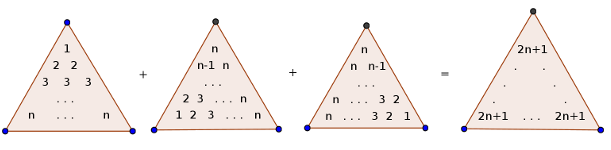
\includegraphics[width=\textwidth]{figure/triangle-proof.png}
\end{minipage}

На языке формул:
\[
  3S = (2n+1) \cdot (1 + 2 + \ldots + n) = (2n+1)n\frac{n+1}{2}.
\]
\end{solution}
\protect \hypertarget {soln:21.2}{}
\begin{solution}{{21.2}}
  Проекцией вектора $(6, 3, 7, 8, 9, 10, 11)$; $a=6$, $b=5$, $c= 9$;
\end{solution}
\protect \hypertarget {soln:21.3}{}
\begin{solution}{{21.3}}
\end{solution}
\protect \hypertarget {soln:21.4}{}
\begin{solution}{{21.4}}
\begin{enumerate}
\item $\chi^2_d$
\item $d$
\item $2d$
\item $\chi^2_{a+b}$
\end{enumerate}
\end{solution}
\protect \hypertarget {soln:21.5}{}
\begin{solution}{{21.5}}
  $Q= Z_1^2$, зная функцию плотности $Z_1$, $f(z_1) = \frac{1}{\sqrt{2\pi}}\exp(-z_1^2/2)$, находим функцию плотности $Q$;
\end{solution}
\protect \hypertarget {soln:21.6}{}
\begin{solution}{{21.6}}
\end{solution}
\protect \hypertarget {soln:21.7}{}
\begin{solution}{{21.7}}
\end{solution}
\protect \hypertarget {soln:21.8}{}
\begin{solution}{{21.8}}
  $\hat Z = \langle Z, z\rangle \cdot v$;
$\hat Z_i = \langle Z, z\rangle \cdot v_i$;
$\Var(\langle Z, z\rangle)=1$; $\Cov(\hat Z_i, \hat Z_j)=v_i v_j \Var( \langle Z, z\rangle)= v_i v_j$;
\end{solution}
\protect \hypertarget {soln:22.1}{}
\begin{solution}{{22.1}}
  Метод максимального правдоподобия:
  \[
    C_n^{Y_{\text{к}}}C_{n-Y_{\text{к}}}^{Y_{\text{щ}}}a^{Y_{\text{к}}}(2a)^{Y_{\text{щ}}}(1-3a)^{Y_{\text{б}}} \to \max_a
  \]
Решая задачу максимизации Кота Матроскина получаем
\[
\hat a_{КМ} = \frac{Y_{\text{к}} + Y_{\text{щ}}}{3n}
\]

Замечаем, что $Y_{\text{к}} + Y_{\text{щ}} \sim Bin(n, 3a)$. Отсюда $\E(\hat a_{\text{КМ}})=a$, $\Var(\hat a_{\text{КМ}}) = \frac{a(1-3a)}{n}$. Оценка несмещённая и состоятельная.

С точки зрения Пса Шарика, неизвестными являются две вероятности, $a$ и $b$. Он решает задачу максимизации по двум переменным. В результате получается вполне себе интуитивная оценка $\hat a_{\text{ПШ}} = Y_{\text{к}}/n$.

\end{solution}
\protect \hypertarget {soln:22.2}{}
\begin{solution}{{22.2}}
Метод правдоподобия: $\max_n \P(S=80)$. Замечаем, что $S \sim Bin\left(100, p=\frac{100}{n}\right)$. Отсюда, $\hat n_{ML} = 125$.

Метод моментов. Рассмотрим $Y_1$, $Y_2$, \ldots, $Y_n$. Величина $Y_i$ равна 1 если при втором отлове $i$-ый заяц оказался с бантом и 0 иначе.

Метод моментов: $\E(Y_i)|_{n=\hat n}=\bar Y$:
\[
\frac{100}{\hat n_{MM}}=\bar Y
\]
Отсюда
\[
\hat n_{MM} = \frac{100}{\bar Y} = \frac{100^2}{S}
\]
\end{solution}
\protect \hypertarget {soln:22.3}{}
\begin{solution}{{22.3}}
\end{solution}
\protect \hypertarget {soln:22.4}{}
\begin{solution}{{22.4}}
\end{solution}
\protect \hypertarget {soln:22.5}{}
\begin{solution}{{22.5}}
\end{solution}
\protect \hypertarget {soln:23.1}{}
\begin{solution}{{23.1}}
  $\hat{\theta}_{ML}=0.25$, $\hat{\theta}_{MM}=0.2$
  $\hat{\theta}_{MM}=\frac{2{,}4-\bar{X}}{7}$
\end{solution}
\protect \hypertarget {soln:23.2}{}
\begin{solution}{{23.2}}
$\hat{a}=\ln(Y_{1})$, $\hat{b}=\ln(Y_{2})-\ln(Y_{1})$
\end{solution}
\protect \hypertarget {soln:23.3}{}
\begin{solution}{{23.3}}
\end{solution}
\protect \hypertarget {soln:23.4}{}
\begin{solution}{{23.4}}
\end{solution}
\protect \hypertarget {soln:23.5}{}
\begin{solution}{{23.5}}
\end{solution}
\protect \hypertarget {soln:23.6}{}
\begin{solution}{{23.6}}
$\hat{a}_{ml}=\sum X_i^2/2n$, $\hat{a}_{mm}=\bar{X}$.
\end{solution}
\protect \hypertarget {soln:23.7}{}
\begin{solution}{{23.7}}
\end{solution}
\protect \hypertarget {soln:23.8}{}
\begin{solution}{{23.8}}
\end{solution}
\protect \hypertarget {soln:23.9}{}
\begin{solution}{{23.9}}
\end{solution}
\protect \hypertarget {soln:23.10}{}
\begin{solution}{{23.10}}
\end{solution}
\protect \hypertarget {soln:23.11}{}
\begin{solution}{{23.11}}
\end{solution}
\protect \hypertarget {soln:23.12}{}
\begin{solution}{{23.12}}
\end{solution}
\protect \hypertarget {soln:23.13}{}
\begin{solution}{{23.13}}
\end{solution}
\protect \hypertarget {soln:23.14}{}
\begin{solution}{{23.14}}
\end{solution}
\protect \hypertarget {soln:23.15}{}
\begin{solution}{{23.15}}
\end{solution}
\protect \hypertarget {soln:23.16}{}
\begin{solution}{{23.16}}
\end{solution}
\protect \hypertarget {soln:23.17}{}
\begin{solution}{{23.17}}
\end{solution}
\protect \hypertarget {soln:23.18}{}
\begin{solution}{{23.18}}
\end{solution}
\protect \hypertarget {soln:23.19}{}
\begin{solution}{{23.19}}
\end{solution}
\protect \hypertarget {soln:23.20}{}
\begin{solution}{{23.20}}
\end{solution}
\protect \hypertarget {soln:23.21}{}
\begin{solution}{{23.21}}
\begin{enumerate}
\item $\E(X_i) = a$, $\E(|X_i|) = 5a/4$
\item $\hat a = 11/30$
\item $\hat a = 26/75$
\item $\hat{a}_{GMM} = 108/325$
\item $\begin{pmatrix}
37 & -44 \\
-44 & 64
\end{pmatrix}$
\end{enumerate}
\end{solution}
\protect \hypertarget {soln:23.22}{}
\begin{solution}{{23.22}}
\end{solution}
\protect \hypertarget {soln:23.23}{}
\begin{solution}{{23.23}}
  $\plim_{n\to\infty} \hat\alpha_{ML}(n) = 0$, не является состоятельной
\end{solution}
\protect \hypertarget {soln:23.24}{}
\begin{solution}{{23.24}}

\end{solution}
\protect \hypertarget {soln:24.1}{}
\begin{solution}{{24.1}}
    \begin{enumerate}
      \item $c=1/n$, да
      \item $c=1/(n+\sigma^2/\mu^2)$, нет, так как $\mu$ и $\sigma$ неизвестны
      \item $\lambda=0$ и $\lambda=\sigma^2/\mu^2$
    \end{enumerate}
  
\end{solution}
\protect \hypertarget {soln:24.2}{}
\begin{solution}{{24.2}}
    \begin{enumerate}
    \item несмещённая, состоятельная, линейная, неэффективная
    \item несмещённая, состоятельная, линейная, неэффективная
    \item несмещённая, несостоятельная, линейная, неэффективная
    \item смещённая, состоятельная, линейная
    \item смещённая, состоятельная, нелинейная
    \item несмещённая, состоятельная, линейная, неэффективная
    \item несмещённая, состоятельная, линейная, эффективная
    \item смещённая, несостоятельная, линейная
    \item смещённая, несостоятельная, нелинейная
    \item несмещённая, состоятельная, линейная, неэффективная
    \end{enumerate}
  
\end{solution}
\protect \hypertarget {soln:24.3}{}
\begin{solution}{{24.3}}
\begin{enumerate}
\item $\hat\theta_{ML} = \max\{ Y_1, Y_2, \ldots, Y_n\}$.
\item Все $Y_i$ меньше $\theta$, значит и $\hat\theta$ всегда меньше $\theta$, значит смещённая.
\item $F_{\hat\theta}(t) = \P(\hat\theta \leq t) = \P(Y_1 \leq t, Y_2 \leq t, \ldots) = (\P(Y_1 \leq t))^n$, $\P(Y_1 \leq t) = t^5/\theta^5$, $f_{\hat\theta}(t) = dF_{\hat\theta}(t)/dt = \frac{5n t^{5n-1}}{\theta^{5n}}$.
\item $\E(\hat\theta) = \frac{5n}{5n+1}\theta$.
\item $\hat\theta_{unbiased} = \frac{5n+1}{5n}\hat\theta$.
\end{enumerate}
\end{solution}
\protect \hypertarget {soln:24.4}{}
\begin{solution}{{24.4}}
\begin{enumerate}
  \item $\hat p$ несмещённая
  \item $\sigma^2 = n p(1-p)$.
  \item $\E(\hat\sigma^2) = (n-1)p(1-p)$, смещённая, $\hat\sigma^2_{unbiased} = \frac{n}{n-1} \hat\sigma^2$.
\end{enumerate}
\end{solution}
\protect \hypertarget {soln:24.5}{}
\begin{solution}{{24.5}}

\end{solution}
\protect \hypertarget {soln:24.6}{}
\begin{solution}{{24.6}}

\end{solution}
\protect \hypertarget {soln:24.7}{}
\begin{solution}{{24.7}}

\end{solution}
\protect \hypertarget {soln:24.8}{}
\begin{solution}{{24.8}}

\end{solution}
\protect \hypertarget {soln:24.9}{}
\begin{solution}{{24.9}}

\end{solution}
\protect \hypertarget {soln:24.10}{}
\begin{solution}{{24.10}}

\end{solution}
\protect \hypertarget {soln:24.11}{}
\begin{solution}{{24.11}}

\end{solution}
\protect \hypertarget {soln:24.12}{}
\begin{solution}{{24.12}}
  Закон распределения $X$ также экспоненциальный, но с другим $\lambda$. Честно находим $\E(X)=\theta/20$, отсюда
  $\hat\theta_{unbiased} = 20X$.
\end{solution}
\protect \hypertarget {soln:24.13}{}
\begin{solution}{{24.13}}

\end{solution}
\protect \hypertarget {soln:24.14}{}
\begin{solution}{{24.14}}
Обе оценки несмещённые, состоятельные. Более эффективна $\hat{\beta}_{2}=\frac{\sum{x_{i}Y_{i}}}{\sum x_{i}^{2}}$.
\end{solution}
\protect \hypertarget {soln:24.15}{}
\begin{solution}{{24.15}}

\end{solution}
\protect \hypertarget {soln:25.1}{}
\begin{solution}{{25.1}}
  $\frac{1}{1.8} - \frac{1}{2.2}$, $[0;10X]$.
\end{solution}
\protect \hypertarget {soln:25.2}{}
\begin{solution}{{25.2}}
\end{solution}
\protect \hypertarget {soln:25.3}{}
\begin{solution}{{25.3}}
\end{solution}
\protect \hypertarget {soln:25.4}{}
\begin{solution}{{25.4}}
\end{solution}
\protect \hypertarget {soln:25.5}{}
\begin{solution}{{25.5}}
\end{solution}
\protect \hypertarget {soln:25.6}{}
\begin{solution}{{25.6}}
Важна при обоих доверительных интервалах. Без предпосылки о нормальности интервал для дисперсии по данным формулам нельзя построить даже при больших $n$. При больших $n$ можно отказаться от предпосылки о нормальности при построении интервала для $\mu$.
\end{solution}
\protect \hypertarget {soln:25.7}{}
\begin{solution}{{25.7}}
\end{solution}
\protect \hypertarget {soln:26.1}{}
\begin{solution}{{26.1}}
к 1/2
\end{solution}
\protect \hypertarget {soln:26.2}{}
\begin{solution}{{26.2}}
  равномерно, $\alpha=0.05$; нет, он резко увеличивает ошибку второго рода
\end{solution}
\protect \hypertarget {soln:26.3}{}
\begin{solution}{{26.3}}
  $\alpha = 1/8$, $\beta = 9/32$
\end{solution}
\protect \hypertarget {soln:26.4}{}
\begin{solution}{{26.4}}
  $\alpha = \P(\cN(0;1) > -0.35) \approx 0.64$, $\beta = \P(\cN(0;1) \leq -1.76) \approx 0.04$.
\end{solution}
\protect \hypertarget {soln:26.5}{}
\begin{solution}{{26.5}}
\end{solution}
\protect \hypertarget {soln:26.6}{}
\begin{solution}{{26.6}}
\end{solution}
\protect \hypertarget {soln:26.7}{}
\begin{solution}{{26.7}}

\end{solution}
\protect \hypertarget {soln:26.8}{}
\begin{solution}{{26.8}}
Критерий Неймана-Пирсона сводится к сравнению $\bar X$ с порогом. При верной $H_0$ величина $\bar X$ распределена $\cN(0; \frac{4}{n})$.
Отсюда искомый критерий имеет вид:
Если $\bar X  \geqslant 0.825$, то гипотеза ${H_0}$ отвергается в пользу гипотезы ${H_a}$.
\end{solution}
\protect \hypertarget {soln:26.9}{}
\begin{solution}{{26.9}}
  Упрощая неравенство из леммы Неймана-Пирсона, получаем критерий: если $X_1\cdot X_2 >t$, то $H_0$ отвергается. Величину $t$ находим из уравнения
\[
\int_0^t (1 - t/x) \, dx = 0.05
\]
\end{solution}
\protect \hypertarget {soln:26.10}{}
\begin{solution}{{26.10}}

\end{solution}
\protect \hypertarget {soln:26.11}{}
\begin{solution}{{26.11}}
\end{solution}
\protect \hypertarget {soln:27.1}{}
\begin{solution}{{27.1}}
При $p_N$ заданном в $H_0$ критерий Пирсона имеет хи-квадрат распределение с двумя степенями свободы.
При оцениваемом $p_N$ критерий Пирсона имеет хи-квадрат распределение с одной степенью свободы.

\url{https://ru.wikipedia.org/wiki/Закон_Харди_—_Вайнберга}
  
\end{solution}
\protect \hypertarget {soln:28.1}{}
\begin{solution}{{28.1}}
$\E(Ay)=A\E(y)$, $\Var(Ay)=A\Var(y)A^T$
\end{solution}
\protect \hypertarget {soln:28.2}{}
\begin{solution}{{28.2}}

\end{solution}
\protect \hypertarget {soln:28.3}{}
\begin{solution}{{28.3}}

\end{solution}
\protect \hypertarget {soln:28.4}{}
\begin{solution}{{28.4}}

\end{solution}
\protect \hypertarget {soln:28.5}{}
\begin{solution}{{28.5}}

\end{solution}
\protect \hypertarget {soln:28.6}{}
\begin{solution}{{28.6}}

\end{solution}
\protect \hypertarget {soln:29.1}{}
\begin{solution}{{29.1}}
Вычтем $2x^2 + 2y^2 + 2z^2 + 2w^2$. Получим, что оптимальное $x=0$. Далее, $z=0$, $y=0$. В итоге $w=1$ или $w=-1$.
\end{solution}
\protect \hypertarget {soln:29.2}{}
\begin{solution}{{29.2}}
\end{solution}
\protect \hypertarget {soln:29.3}{}
\begin{solution}{{29.3}}
\end{solution}
\protect \hypertarget {soln:29.4}{}
\begin{solution}{{29.4}}
\end{solution}
\protect \hypertarget {soln:29.5}{}
\begin{solution}{{29.5}}
$(5+4+1)=10$; длины — $\sqrt{5}\cdot\sqrt{99}$, $\sqrt{4}\cdot\sqrt{99}$, $\sqrt{1}\cdot\sqrt{99}$; выборочные дисперсии — $5$, $4$, $1$; $(5+4)/10=0.9$.
\end{solution}
\protect \hypertarget {soln:29.6}{}
\begin{solution}{{29.6}}
\end{solution}
\protect \hypertarget {soln:30.1}{}
\begin{solution}{{30.1}}
  
\end{solution}
\protect \hypertarget {soln:30.2}{}
\begin{solution}{{30.2}}
  
\end{solution}
\protect \hypertarget {soln:30.3}{}
\begin{solution}{{30.3}}
  
\end{solution}
\protect \hypertarget {soln:31.1}{}
\begin{solution}{{31.1}}
$C_{20}^2\cdot 18$.
\end{solution}
\protect \hypertarget {soln:31.2}{}
\begin{solution}{{31.2}}
  $1+x+x^2+x^3+x^4=(1-x^5)/(1-x)$
  $1+x+x^2+x^3+\ldots = 1/(1-x)$
  $(1+x)^4$
\end{solution}
\protect \hypertarget {soln:31.3}{}
\begin{solution}{{31.3}}
\end{solution}
\protect \hypertarget {soln:31.4}{}
\begin{solution}{{31.4}}
\end{solution}
\protect \hypertarget {soln:31.5}{}
\begin{solution}{{31.5}}
  0 с вероятностью 1/4 и 1 с вероятностью 3/4
\end{solution}
\protect \hypertarget {soln:31.6}{}
\begin{solution}{{31.6}}
  да, сможет!
\end{solution}
\protect \hypertarget {soln:31.7}{}
\begin{solution}{{31.7}}
$F_n = F_{n-1} + F_{n-2}$.
Запишем разложения для $g(x)$, $xg(x)$ и $x^2 g(x)$ друг под другом. Вычитаем. Получаем, что $g(x) = x/(1-x-x^2)$.

Указанная дробь — это и есть производящая функция при маленьком $x$.

Производящая функция представима в виде суммы:
\[
g(x) = \frac{1}{\sqrt{5}}\left( \frac{a}{x+a} - \frac{b}{x+b}  \right),
\]
где $a=(1-\sqrt{5})/2$, $b=(1+\sqrt{5})/2$.
\end{solution}
\protect \hypertarget {soln:31.8}{}
\begin{solution}{{31.8}}
Замечаем, что $h_2(t)=h_1(t)\cdot h_1(t)$. После первого шага:
\[
h_1(t) = 0.7t + 0.3th^2_1(t)
\]
\end{solution}
\protect \hypertarget {soln:31.9}{}
\begin{solution}{{31.9}}

\end{solution}
\protect \hypertarget {soln:32.1}{}
\begin{solution}{{32.1}}
\end{solution}
\protect \hypertarget {soln:32.2}{}
\begin{solution}{{32.2}}
\end{solution}
\protect \hypertarget {soln:33.1}{}
\begin{solution}{{33.1}}
  Если величина $X$ равновероятно принимает $k$ значений, то спутанность равна $k$. У равномерной на $[0;a]$ спутанность равна $a$.
\end{solution}
\protect \hypertarget {soln:33.2}{}
\begin{solution}{{33.2}}
\end{solution}
\protect \hypertarget {soln:33.3}{}
\begin{solution}{{33.3}}
\end{solution}
\protect \hypertarget {soln:33.4}{}
\begin{solution}{{33.4}}
\end{solution}
\protect \hypertarget {soln:33.5}{}
\begin{solution}{{33.5}}
\end{solution}





\addcontentsline{toc}{section}{Хэштэги}
\printindex % [heading=none]


% \section*{Источники мудрости}

\nocite{buzun2015stochastic}



\addcontentsline{toc}{section}{Источники мудрости}
\printbibliography[heading=none]


\end{document}
